\documentclass[twocolumn,secnumarabic,amssymb, nobibnotes, aps, prl,
superscriptaddress, nobalancelastpage]{revtex4}
\newcommand{\revtex}{REV\TeX\ }
\newcommand{\classoption}[1]{\texttt{#1}}
\newcommand{\macro}[1]{\texttt{\textbackslash#1}}
\newcommand{\m}[1]{\macro{#1}} \newcommand{\env}[1]{\texttt{#1}}
\setlength{\textheight}{9.5in} \usepackage{graphicx}
\setlength{\belowcaptionskip}{6pt}
\usepackage{amsmath} \usepackage{braket} \usepackage{epsfig}
\usepackage{upgreek}
\usepackage{textcomp}
\usepackage[free-standing-units]{siunitx}
\usepackage{xcolor}

\newcolumntype{N}{>{\centering\arraybackslash}m{1.3in}}
\newcolumntype{M}{>{\centering\arraybackslash}m{1.0in}}
\newcolumntype{G}{>{\centering\arraybackslash}m{0.5in}}
\newcolumntype{R}{>{\raggedleft\arraybackslash}m{0.4in}}

\newcommand{\tot}{\ensuremath{\sigma_{tot}}}
\newcommand{\totRD}{\ensuremath{\sigma_{A,A'}}(E)}
\newcommand{\rxn}{\ensuremath{\sigma_{rxn}}}
\newcommand{\el}{\ensuremath{\frac{\lowercase{d}\sigma}{\lowercase{d}\Omega}}}

\newcommand{\oSix}{\ensuremath{^{16}}O}
\newcommand{\oSeven}{\ensuremath{^{17}}O}
\newcommand{\oEight}{\ensuremath{^{18}}O}
\newcommand{\oSixEight}{\ensuremath{^{16,18}}O}

\newcommand{\neEight}{\ensuremath{^{18}}N\lowercase{e}}

\newcommand{\caForty}{\ensuremath{^{40}}C\lowercase{a}}
\newcommand{\caEight}{\ensuremath{^{48}}C\lowercase{a}}
\newcommand{\caAughtEight}{\ensuremath{^{40,48}}C\lowercase{a}}

\newcommand{\niSix}{\ensuremath{^{56}}N\lowercase{i}}
\newcommand{\niEight}{\ensuremath{^{58}}N\lowercase{i}}
\newcommand{\niSixty}{\ensuremath{^{60}}N\lowercase{i}}
\newcommand{\niOne}{\ensuremath{^{61}}N\lowercase{i}}
\newcommand{\niTwo}{\ensuremath{^{62}}N\lowercase{i}}
\newcommand{\niFour}{\ensuremath{^{64}}N\lowercase{i}}
\newcommand{\niEightFour}{\ensuremath{^{58,64}}N\lowercase{i}}
\newcommand{\niNat}{\ensuremath{^{\text{nat}}}N\lowercase{i}}

\newcommand{\rhThree}{\ensuremath{^{103}}R\lowercase{h}}

\newcommand{\snTwelve}{\ensuremath{^{112}}S\lowercase{n}}
\newcommand{\snFourteen}{\ensuremath{^{114}}S\lowercase{n}}
\newcommand{\snFifteen}{\ensuremath{^{115}}S\lowercase{n}}
\newcommand{\snSixteen}{\ensuremath{^{116}}S\lowercase{n}}
\newcommand{\snSeventeen}{\ensuremath{^{117}}S\lowercase{n}}
\newcommand{\snEighteen}{\ensuremath{^{118}}S\lowercase{n}}
\newcommand{\snNineteen}{\ensuremath{^{119}}S\lowercase{n}}
\newcommand{\snTwenty}{\ensuremath{^{120}}S\lowercase{n}}
\newcommand{\snTwo}{\ensuremath{^{122}}S\lowercase{n}}
\newcommand{\snFour}{\ensuremath{^{124}}S\lowercase{n}}
\newcommand{\snTwelveFour}{\ensuremath{^{112,124}}S\lowercase{n}}
\newcommand{\snNat}{\ensuremath{^{\text{\lowercase{nat}}}}S\lowercase{n}}
\newcommand{\snTwelveNatFour}{\ensuremath{^{112,\text{nat},124}}S\lowercase{n}}

\newcommand{\pbEight}{\ensuremath{^{208}}P\lowercase{b}}
\newcommand{\pbNat}{\ensuremath{^{\text{\lowercase{nat}}}}P\lowercase{b}}

% shell labels
\newcommand{\sOne}{s\ensuremath{_{\frac{1}{2}}}}
\newcommand{\pThree}{p\ensuremath{_{\frac{3}{2}}}}
\newcommand{\pOne}{p\ensuremath{_{\frac{1}{2}}}}
\newcommand{\dFive}{d\ensuremath{_{\frac{5}{2}}}}
\newcommand{\dThree}{d\ensuremath{_{\frac{3}{2}}}}
\newcommand{\fSeven}{f\ensuremath{_{\frac{7}{2}}}}
\newcommand{\fFive}{f\ensuremath{_{\frac{5}{2}}}}
\newcommand{\gNine}{g\ensuremath{_{\frac{9}{2}}}}
\newcommand{\gSeven}{g\ensuremath{_{\frac{7}{2}}}}
\newcommand{\hEleven}{h\ensuremath{_{\frac{11}{2}}}}

\newcommand{\tZero}{T\ensuremath{_{0}}}



\begin{document}

\begin{abstract}
    The neutron total cross sections \tot\ of $^{16,18}$O,
    $^{58,nat,64}$Ni, $^{103}$Rh, and $^{112,nat,124}$Sn have been measured at the Los Alamos
    Neutron Science Center (LANSCE) at intermediate energies (3 $\leq E_{n}
    \leq$ 450 MeV) by
    leveraging waveform digitizer technology. The results are in good agreement
    with previous measurements that used analog techniques,
    excepting small deviations at high energies. These data
    continue the campaign of
    \tot\ measurements we initiated with the case study of $^{40,48}$Ca in 2009.
    The \tot\ relative differences between isotopes are presented,
    revealing additional information about
    the isovector components needed for an accurate optical model (OM)
    description away from stability. Digitizer-enabled \tot-measurement
    techniques are discussed and a series of Dispersive Optical Model (DOM)
    analyses using these new data is presented, validating the DOM for modeling light
    systems (\oSixEight) and systems with open neutron shells (\niEightFour\ and \snTwelveFour).
    Our results indicate that proton and neutron reaction and total cross
    section data on neutron-rich isotopes are of great value for constraining
    asymmetry-dependent nuclear structural quantities otherwise difficult
    to observe experimentally.
\end{abstract}

\title{Isotopically-Resolved Neutron Total Cross Sections At
Intermediate Energies}

\author{C.~D.~Pruitt}  \email[Corresponding author:]{cdpruitt@wustl.edu}
\author{R.~J.~Charity}
\affiliation{Department of Chemistry, Washington University, St. Louis, MO 63130}
\author{L.~G.~Sobotka}
\affiliation{Department of  Chemistry, Washington University, St. Louis, MO 63130, USA}
\affiliation{Department of  Physics, Washington University, St. Louis, MO 63130, USA}
\author{D. E.~M.~Hoff}  
\affiliation{Department of Chemistry, Washington University, St. Louis, MO 63130}
\altaffiliation{Present Address: \textit{Department of Physics, University of
        Massachusetts-Lowell and
Astronomy, Michigan State University, East Lansing, MI 48824, USA}}

\author{K.~W.~Brown} \altaffiliation{Present Address: \textit{National
        Superconducting Cyclotron Laboratory, Departments of Physics and
Astronomy, Michigan State University, East Lansing, MI 48824, USA}}
\author{J.~M.~Elson}
\affiliation{Department of Chemistry, Washington University, St. Louis, MO 63130}

\author{M.C.~Atkinson}
\author{W.H.~Dickhoff}
\affiliation{Department of Physics, Washington University, St. Louis, MO 63130}

\author{H. Y. Lee}
\author{M. Devlin}
\author{N. Fotiadis}
\author{S. Mosby}
\affiliation{Los Alamos National Lab, Los Alamos, NM 87545, USA}
\maketitle

Neutron scattering is a direct, Coulomb-insensitive tool for probing the nuclear
environment. The simplest neutron-nucleus interaction quantity is 
the neutron total cross section, \tot, which provides fundamental information about
nuclear size and the ratio of elastic-to-inelastic components of nucleon 
scattering. Additionally, \tot\ data are thought to be tightly correlated with
a variety of structural nuclear properties of great interest
including the neutron skin of neutron-rich nuclei
\cite{Mahzoon2017} and thus the density dependence of the symmetry energy $L$,
an essential equation-of-state (EOS) input for neutron star
structure calculations \cite{Fattoyev2012, Vinas2014, Brown2000}.

In the crudest approximation, the ``strongly-absorbing sphere'' picture
explains the dependence of \tot\ on the size of the target nucleus and on the
energy of the incident neutron as a consequence of simple size-scaling:
\begin{equation} \label{SASAbsolute}
    \sigma_{tot}(E) = 2\pi(R + \lambdabar)^{2},
\end{equation}
where $R=r_{0}A^{\frac{1}{3}}$ and $\lambdabar$ is the reduced wavelength
of the incident neutron with energy $E$ in the center of mass \cite{Fernbach1949, Satchler1980}. 
%To compare \tot\ for two different targets of masses A and A$'$, the relative
%difference \totRD\ is useful:
%\begin{equation} \label{SASRelDiff}
%    \begin{split}
%        \totRD\ & \equiv
%    \frac{\sigma_{A}-\sigma_{A'}}{\sigma_{A}+\sigma_{A'}} \\
%    & =
%    \frac{r_{0}^{2}(A^{\frac{2}{3}}-A'^{\frac{2}{3}}) +
%    2\lambdabar r_{0}(A^{\frac{1}{3}}-A'^{\frac{1}{3}})}
%    {r_{0}^{2}(A^{\frac{2}{3}}+A'^{\frac{2}{3}}) +
%    2\lambdabar r_{0}(A^{\frac{1}{3}}+A'^{\frac{1}{3}}) + 2\lambdabar^{2}},
%    \end{split}
%\end{equation}
While on \textit{average}, experimental \tot\ data comport with this na\"ive
model, the most prominent feature of experimental \tot\ data is the oscillatory
behavior centered about the average of Eq. (\ref{SASAbsolute}), visible in Fig.
\ref{SASphereVsExperiment}.

\begin{figure}
    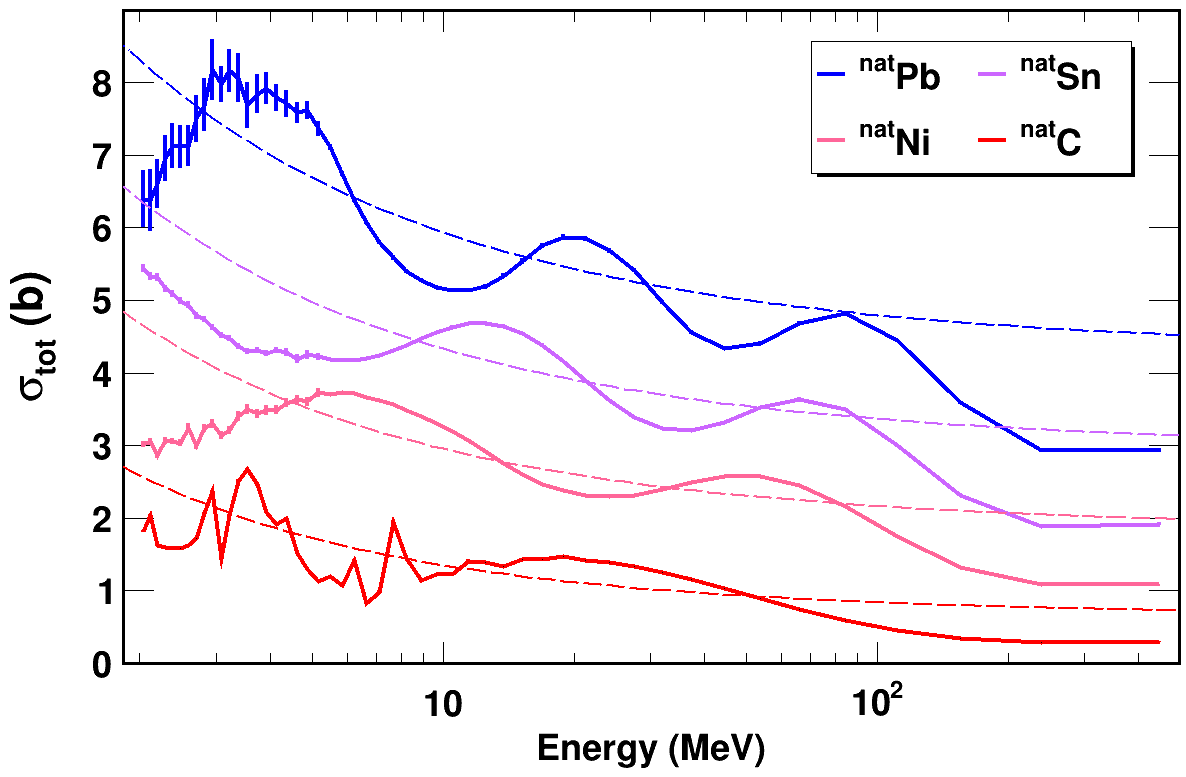
\includegraphics[width=\linewidth]{figures/ExampleTCS.png}
    \caption{
        (Color online) Experimental \tot\ data are shown from 2-500
        MeV for nuclides from A=12 to A=208
        \cite{Finlay1993, Schwartz1974, Poenitz1983, Abfalterer2000, Abfalterer2001}.
        Predictions for \tot\ given by the ``strongly-absorbing sphere'' (SAS)
        model, Eq. (\ref{SASAbsolute}), are shown as thin dashed lines for each nucleus.
        Regular oscillations about the SAS model are visible
        as is the trend for the oscillation
        maxima and minima to shift to \textit{higher} energies as A is increased.
    }
    \label{SASphereVsExperiment}
\end{figure}
Peterson \cite{Peterson1962} interpreted these oscillations as the 
result of a phase shift between neutron partial waves passing \textit{around} the 
nucleus (thus undergoing no phase shift) and waves passing
\textit{through} the nuclear potential, where they are refracted and exhibit a 
retardation of phase (an illustration is available in \cite{Satchler1980}).
This explanation was termed the 
``nuclear Ramsauer effect'' by Carpenter and Wilson \cite{Carpenter1959} based on 
the analogous effect seen in electron scattering on noble gases.

Following Angeli and Csikai \cite{Angeli1970}, this explanation can be
incorporated by imbuing the strongly-absorbing sphere relations
with a sinusoidal term:
\begin{equation} \label{OscillatoryModel}
    \tot = 2\pi (R+\lambdabar)^{2}(1 - \rho \cos(\delta))
\end{equation}
where $\rho = e^{-\operatorname{Im}(\Delta)}$ and $\delta =
\operatorname{Re}(\Delta)$, $\Delta$ being the phase difference between a
partial wave traveling
around and traveling through the nucleus. The large amplitude of the
oscillations suggests that elastic scattering accounts for a
significant fraction of the total cross section, in turn implying a 
larger mean free path for neutrons through the nucleus 
than might otherwise be expected in the absence of Pauli blocking
\cite{Mohr1955, Feshbach1958}.
Continuing, if we approximate the nucleus with a
real spherical potential of radius $R$ and depth $U$, the total phase shift $\delta$ is:
\begin{equation} \label{phaseShift}
    \delta =
    \frac{\overline{C}\left(\left[{\frac{E+U}{E}}\right]^{\frac{1}{2}}-1\right)}{\lambdabar}
\end{equation}
where $\overline{C} = \frac{4}{3}R$ is the average chord length through the
sphere \cite{Angeli1970}. Rearranging Eq. (\ref{phaseShift}) in terms of A and E and
discarding leading constants yields:
\begin{equation}
    \delta \propto A^{\frac{1}{3}}\times\left(\sqrt{E+U}-\sqrt{E}\right)
\end{equation}
This form reveals an important relation: as A is increased, to maintain constant 
phase $\delta$, E must also increase \cite{Satchler1980, Peterson1962}. 
This is contrary to a typical resonance condition where an integer number of wavelengths
are fit inside a potential; in that case, to maintain constant phase as A is increased,
E must be \textit{decreased}. Thus these \tot\ oscillations have been referred to as
``anti-resonances'' or ``echoes'' \cite{Satchler1980, McVoy1967}.
Other authors \cite{Ahmad1973} have
exposed weaknesses in Angeli and Csikai's interpretation of
Eq. (\ref{OscillatoryModel}) and have provided a more general semi-empirical
equation for \tot. However, Eq. (\ref{OscillatoryModel}) is a valuable starting
point for connecting \tot\ with the depth and shape of the nuclear
potential as experienced by neutrons.

By including additional surface, spin-orbit, and other terms, optical models (OMs) have been 
used to successfully reproduce the general features of all manner of single-nucleon scattering 
data across the chart of nuclides up to several hundred MeV \cite{Perey1976,
CH89, KoningDelaroche}. However, despite the excellent agreement with experiment, optical models
involve the interaction of many partial waves with many sometimes-opaque terms
in the potential, complicating intuitive understanding of the underlying
physics at play. In particular, the isovector components of optical potentials
are quite difficult to constrain as they depend on both proton and neutron 
scattering data, one or both of which are often unavailable. For example,
when Dietrich et al. conducted an analysis of neutron total cross section
differences between W isotopes, including standard isovector terms in their
optical potential actually worsened the reproduction of the experimental
relative differences, an
illustration of how poorly these isovector components are known \cite{Dietrich2003}.

With these considerations in mind, our present goal is twofold: first, to
provide new isotopically-resolved \tot\ data useful for identifying the 
dependence of optical 
potential terms on nuclear asymmetry; and second, conduct a Dispersive Optical Model
(DOM) analysis of these new \tot\ data along with a large corpus of scattering
and bound-state data to extract structural quantities (neutron skin
thicknesses, spectroscopic factors) for several cornerstone, closed-proton-shell nuclei.
Key findings of this DOM analysis are presented in the companion paper \cite{Pruitt2020PRL}.

\section{Experimental Considerations}
By scattering secondary radioactive beams off of hydrogen targets in inverse
kinematics, proton-scattering experiments are possible even on highly unstable
nuclides. Because neutrons themselves must be generated as a
secondary radioactive beam, neutron-scattering experiments are restricted to
normal kinematics and \tot\ measurements are possible only for relatively stable
nuclides that can be formed into a target. At present, \tot\ measurements above
the resonance region on nuclides with short half-lives (shorter than the timescale of
days) are technically infeasible for this reason, though a handful have been carried out on
samples with half-lives in the tens to thousands of years \cite{Poenitz1983,
Phillips1980, Foster1971}.

Traditionally, \tot\ measurements have relied on analog techniques for recording
events, techniques that suffer from a large per-event deadtime of
up to several $\micro\second$. Thus for a typical intermediate-energy \tot\ measurement
with dozens or hundreds of energy bins, achieving statistical uncertainty at the
level of 1\% requires a thick sample to attenuate a sizable fraction of the
incident neutron flux. For cross sections in the 1-10 barn range, this means
sample masses of tens of grams \cite{Finlay1993, Abfalterer2001}.
Producing an isotopically-enriched sample of this size is often
prohibitively expensive; indeed, a literature search for isotopically-resolved
\tot\ measurements revealed a paucity of data from 1-300 MeV, even for
closed-shell isotopes of special importance like $^{3,4}$He, \oEight, \niFour,
\snTwelveFour, and $^{204}$Pb (see Fig. 1.3 from \cite{IsotopicCrossSectionTable}).

Recent developments in waveform digitizer technology have made it
possible to reduce the per-event deadtime by an order of magnitude or more,
enabling a corresponding reduction in the necessary sample size. In 2008, we
embarked on a campaign of \tot\ measurements on isotopically-enriched samples
using these new technical capabilities,
starting with $^{40,48}$Ca from $15 \leq E_{n} \leq 300$ MeV \cite{Shane2010}.
The data from that measurement were incorporated into a comprehensive
Dispersive Optical Model (DOM) analysis \cite{Mueller2011, Mahzoon2014,
MahzoonPhDThesis} that yielded proton and neutron spectroscopic factors, charge
radii, and initial estimates of the neutron skins \cite{Mahzoon2017}
for these nuclei.
Here we advance that program by providing \tot\ results for
the important closed-shell nuclides
$^{16,18}$O, $^{58,64}$Ni, and $^{112,124}$Sn. We also present a measurement
on a very thin sample of the naturally-monoisotopic $^{103}$Rh to demonstrate that
\tot\ experiments over a broad energy range using minute amounts of material are feasible.

\section{Experimental Details}
All \tot\ measurements were carried out at the 15R
beamline at the Weapons Neutron Research (WNR) facility of the Los Alamos
Neutron Science Center (LANSCE) during two run cycles (November 2016 and
September 2017). Our experiment was modeled on previous
\tot\ measurements at WNR \cite{Finlay1993,Abfalterer2001,Shane2010}.
At WNR,
broad-spectrum neutrons up
to $\approx$700 MeV are generated by impinging proton pulses onto a water-cooled, 7.5
cm-long tungsten target (see Fig. \ref{ExperimentalApparatus}). Before the beam
enters the experimental area, a
permanent magnet deflects all charged particles generated by the proton pulses, 
allowing only neutrons and $\gamma$ rays to reach the flight path. At the
entrance to the flight path, the beam was collimated to 0.200 inches using steel
donuts with a total thickness of 24 inches and hardened using a plug of Hevimet (90\% W, 6\% 
Ni, 4\% Cu by weight) inserted at the upstream entrance of the
collimation stack. After collimation, the beam passed successively through a flux 
monitor, the sample of interest, a veto detector, and finally the 
time-of-flight (TOF) detector approximately 25 meters from the neutron source.
All detectors consisted of BC-400 fast scintillating plastic mated with 
photomultiplier tubes (PMTs) and encased in either a plastic or
an aluminum housing. The flux monitor and veto detector each had
scintillator thicknesses of 0.25 inch and the TOF detector had a
scintillator thickness of 1 inch. Signals from all detectors and
the target changer were relayed to a 500-MHz CAEN DT-5730 waveform digitizer
running custom software. To improve time resolution, the TOF detector used two
PMTs (one left, one right) mated to the plastic scintillator and the PMTs' signals were 
summed before digitization.

\begin{figure}
    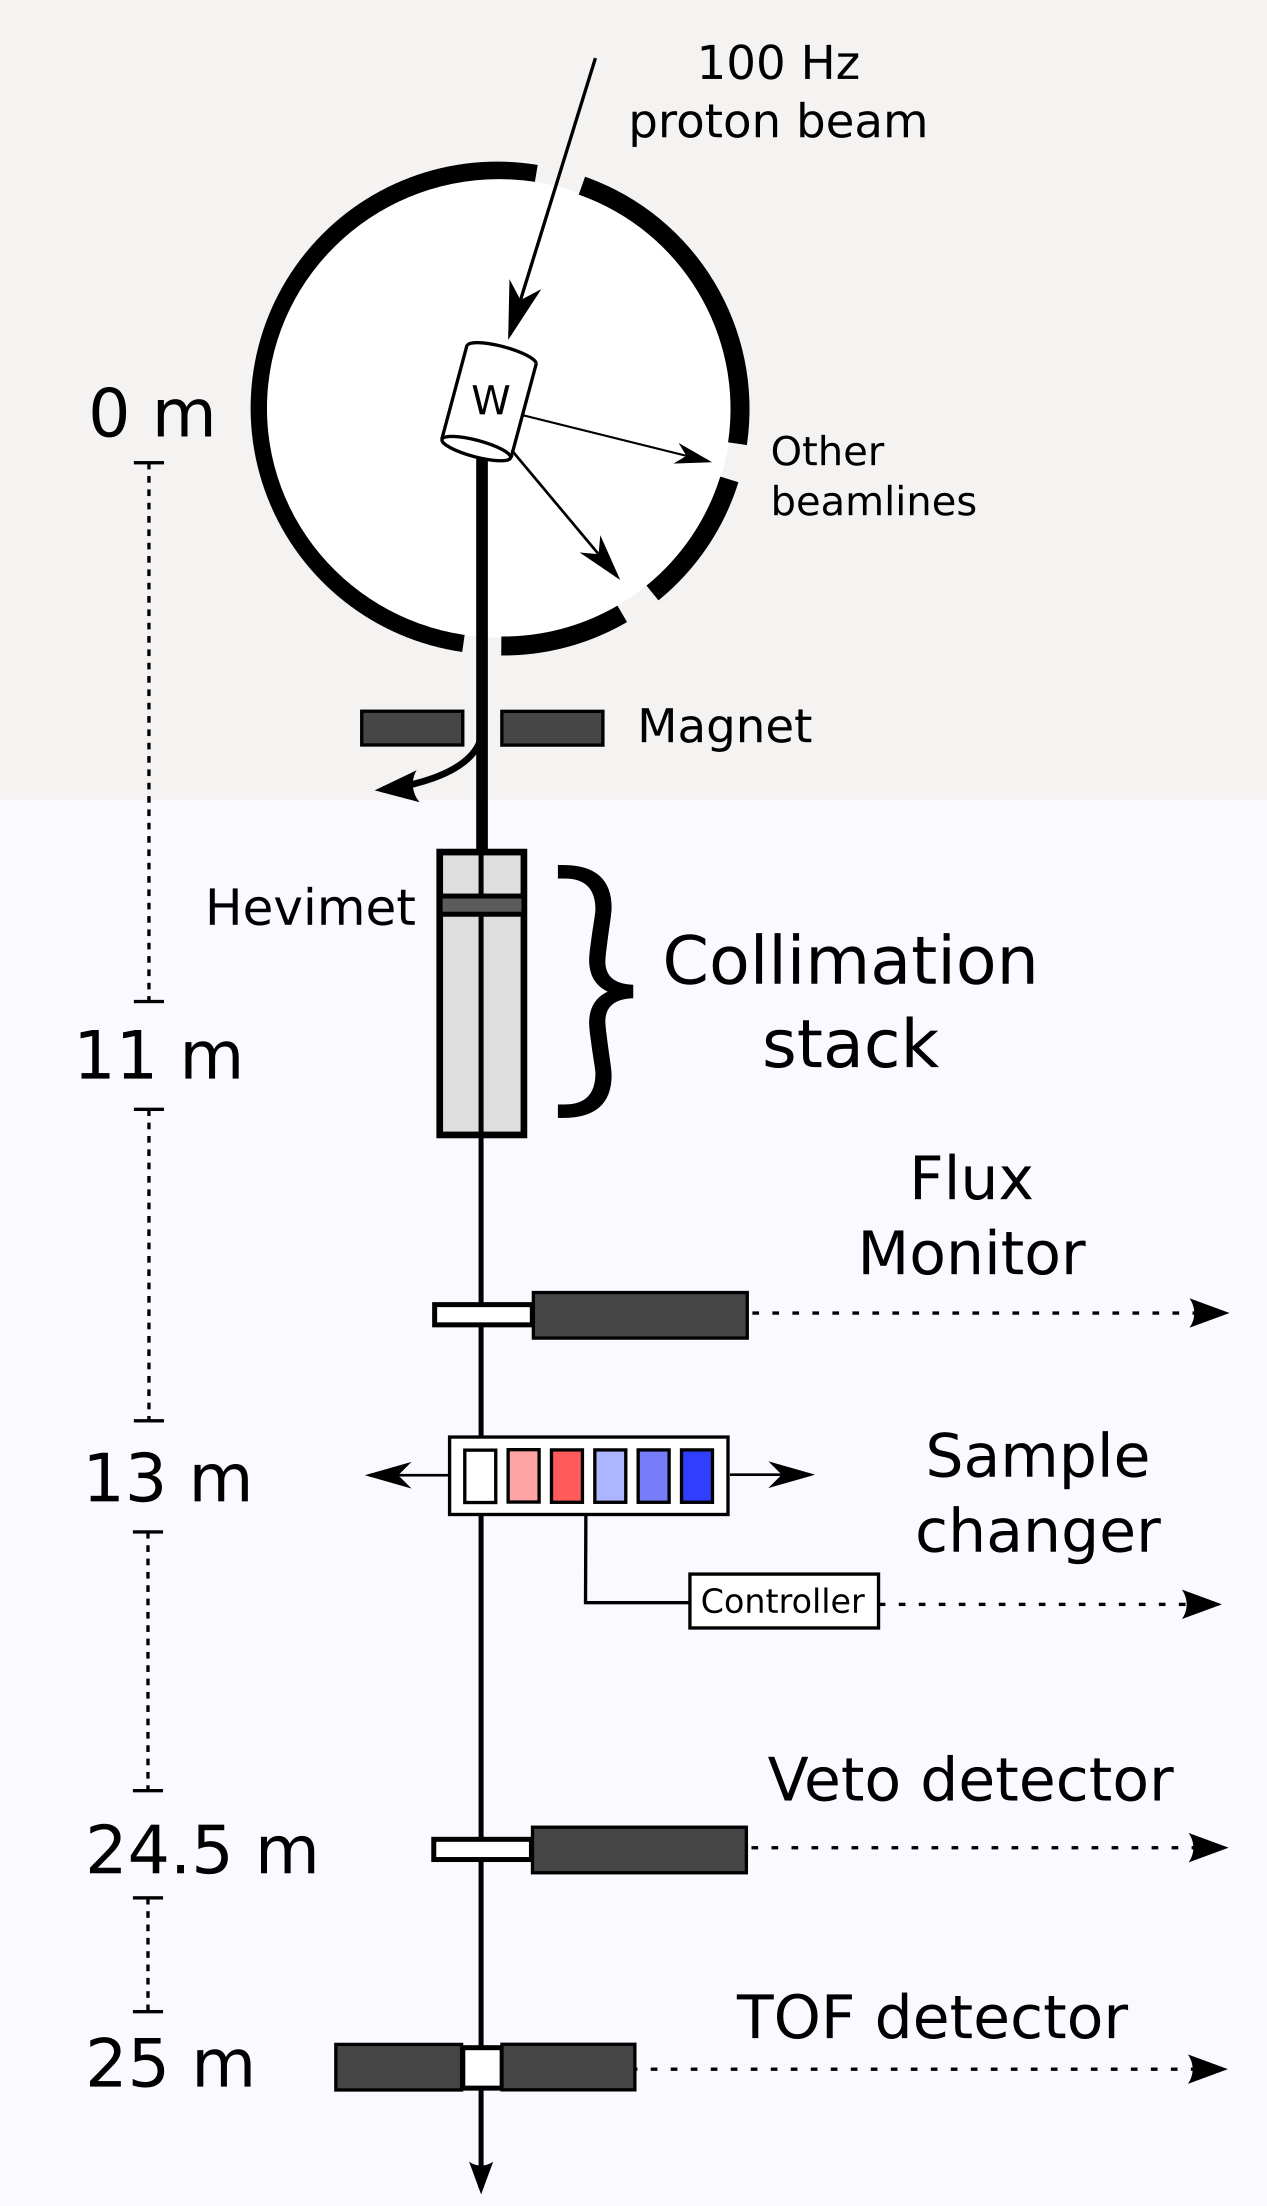
\includegraphics[width=0.3\textwidth]{figures/ExperimentalSetup.png}
    \caption{(Color online) Experimental configuration at WNR facility.
        Samples are cycled into and out of the beam
        using a linear actuator with a period of 150 seconds. Times-of-flight (TOFs) are
    determined by the TOF detector and used to calculate neutron energy.}
    \label{ExperimentalApparatus}
\end{figure}

\begin{figure}
    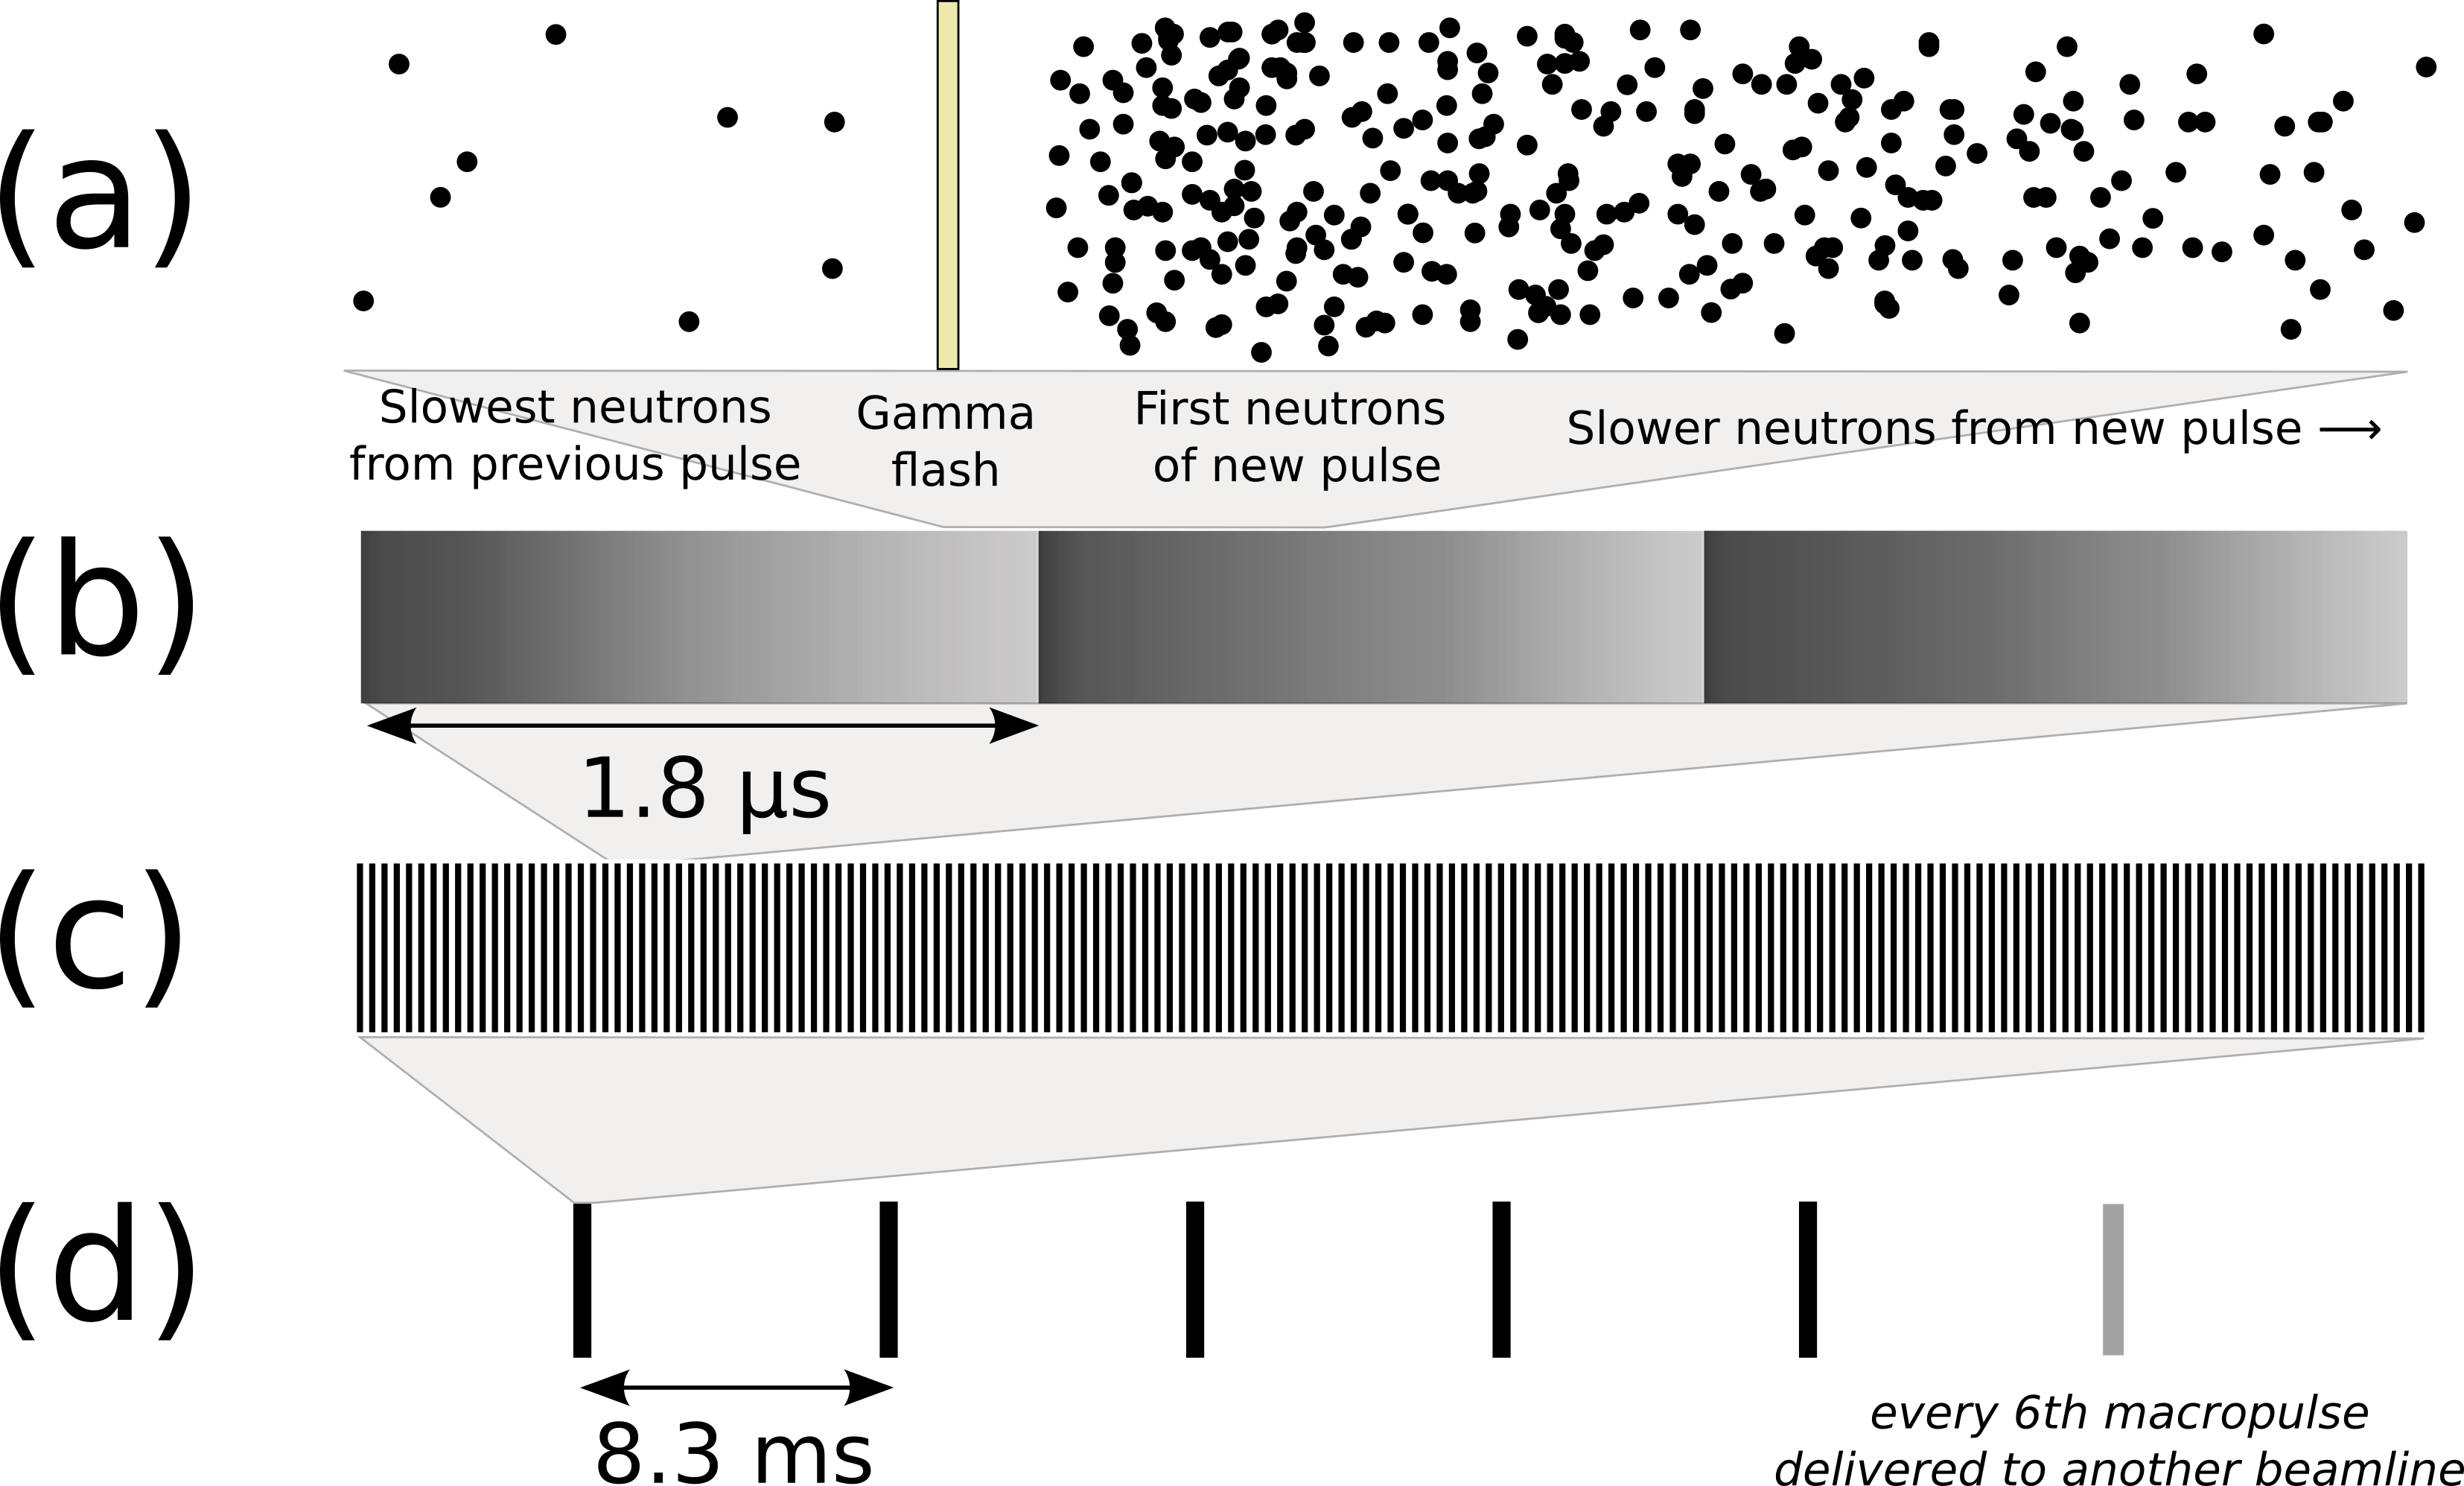
\includegraphics[width=\linewidth]{figures/beamStructure.png}
    \caption{(Color online) Neutron beam structure at WNR facility.
        ``Macropulses'' of protons (row d) are delivered to
        WNR's tungsten Target 4, where they generate neutrons by spallation.
        Each macropulse consists of
        $\approx$350 proton ``micropulses'' (row c). Neutrons
        from each micropulse (row b) disperse in
        time as they travel along the flight path so that $\gamma$ rays and high-energy 
    neutrons catch up to low-energy ones from the previous pulse (row a).}
    \label{BeamStructure}
\end{figure}

The particular neutron beam structure at WNR dictates the energy range
achievable for \tot\ measurements (see Fig. \ref{BeamStructure}).
Proton pulse trains, called ``macropulses'', are delivered to the tungsten target at 120 Hz.
Each macropulse consists of ~350 individual proton pulses, called
``micropulses'', spaced 1.8 
\micro\second\ apart. Each micropulse consists of a single thin proton packet
that generates $\gamma$ rays and neutrons within a tight
temporal-spatial range. As neutrons from this micropulse travel along the beam path, 
high energy neutrons separate in time from lower-energy neutrons so that neutron
energy can be determined by standard TOF techniques (see \cite{Moore1980} for details).
Because the $\gamma$ rays and high-energy neutrons from later micropulses can
overtake slower neutrons from an earlier micropulse, the distance of the TOF
detector from the neutron source determines both the minimum neutron energy that can be 
unambiguously resolved and the maximum instantaneous neutron flux, critical to correcting
for per-event deadtime.

A programmable sample changer with six positions
was used to cycle each sample into the beam at a regular interval of 150 seconds 
per sample. Once per macropulse, an analog signal from the sample changer
was recorded to indicate its current position.
The flux monitor was used to correct for variations in beam flux between 
macropulses. The veto detector suppressed events from charged-particle production 
in the samples and in air along the flight path.

Custom digitizer software was used to run the 
digitizer in two complementary modes, referred to as ``DPP mode'' and ``Waveform 
mode''. In DPP mode, triggers were initiated by the digitizer's onboard
peak-sensing firmware. For each trigger, several quantities were recorded: the trigger 
timestamp, two charge integrals over the detected peak with different
integration ranges (32 ns for the short integral, 100 ns for the long integral),
and a 96-ns portion of the raw digitized waveform, referred to as a ``wavelet''.
DPP mode was used for the vast majority of the 
experiment and accounts for $\approx$99\% of the total data volume. In waveform mode, 
the digitizer performs no peak-sensing and was externally triggered. Upon 
triggering, the trigger timestamp and a very long wavelet (60 $\micro\second$) 
were recorded. While waveform mode data accounts for only $\approx$1\% of the total data, 
the instantaneous data rate is much higher than in DPP 
mode because hundreds of $\micro\second$ of consecutive waveform samples are 
stored. Roughly once every three seconds, the digitizer was switched to 
waveform mode for one macropulse, then switched back to DPP mode as quickly as
possible (10-40 ms, depending on run configuration).  

Except for the O and Rh samples, all samples were prepared as right
cylinders 8.25 mm in diameter and ranging from 10-27 mm in length (see
Table \ref{SampleCharacteristics} for sample characteristics and Fig. \ref{SamplesImage}
for sample images). For each element under study, a natural-abundance sample
was also prepared as were two natural C
samples and a natural Pb sample, useful for benchmarking against
literature data. The samples
were inserted into styrofoam sleeves and seated in the cradles of the sample
changer. This design minimizes the amount of non-target mass proximate to the
neutron beam path. Our samples were generally
much smaller than those used in previous measurements;
for example, the Ni and Sn samples used in \cite{Abfalterer2001,
Finlay1993} had areal densities of 1.515 and 0.5475
$\frac{mol}{cm^{2}}$, respectively, 12.7 and 6.5 times larger than for our
Ni and Sn samples. 

\begin{table}[tb]
    \centering
    %\addtolength{\tabcolsep}{-1pt}
    \begin{tabular}{c c c c c c c}
        \small Isotope & Length & Diam. & Mass & $\rho_{\text{A}}$ & NA & SP\\
        \hline
        $^{\text{nat}}$C& 13.66(2)& 8.260(5)& 1.2363& 0.1921(1)& -& -\\
        $^{\text{nat}}$C& 27.29(2)& 8.260(5)& 2.4680& 0.3835(2)& -& -\\
        \\
        H$_{2}$O& 20.00(1)& 8.92(1)& 1.2461& 0.1107(3)& -& - \\
        D$_{2}$O& 20.00(1)& 8.92(1)& 1.3852& 0.1107(3)& 0.02& 99.9\\
        H$_{2}$$^{18}$O& 20.00(1)& 8.92(1)& 1.3844& 0.1107(3)& 0.20& 99.9\\
        \\
        $^{58}$Ni& 7.97(3)& 8.18(2)& 3.6438& 0.1197(3)& 68.1& 99.6 \\
        $^{\text{nat}}$Ni& 8.00(3)& 8.20(2 & 3.6898& 0.1192(3)& - & -\\
        $^{64}$Ni& 7.96(2)& 8.20(4)& 3.9942& 0.1192(6)& 0.93& 92.2\\
        \\
        $^{103}$Rh& 2.03(1)& 10.20(2)& 2.8359& 0.02426(4)& 100& 99.9\\
        \\
        $^{112}$Sn& 13.65(3)& 8.245(5)& 4.9720& 0.08332(5)& 0.97& 99.9\\
        $^{\text{nat}}$Sn& 13.68(3)& 8.245(5)& 5.3263& 0.08414(5)& - & -\\
        $^{124}$Sn& 13.73(3)& 8.245(5)& 5.5492& 0.08399(5)& 5.79& 99.9\\
        \\
        $^{\text{nat}}$Pb& 10.07(2)& 8.27(1)& 6.130& 0.05508(6)& -& -\\
        \hline
    \end{tabular}
    \centering
    \caption{Physical characteristics of samples used for neutron \tot\ measurements.
        The length and diameter of the sample cylinders are given in
        \milli\meter, and the sample masses are in grams. To calculate cross sections, the relevant
        ``sample thickness'' is the areal density of nuclei
        $\rho_{\text{A}}$, equivalent to the volumetric number density times
        the length of the sample, with units $\frac{mol}{cm^{2}_{ }}$. For liquid
        samples H$_{2}^{\text{nat}}$O, D$_{2}^{\text{nat}}$O, and H$_{2}^{18}$O,
        the length and diameter given are for the interior of the vessels
        used to hold the samples and the masses listed are calculated based on 
        literature values for the density of each sample at 25 C.
        For enriched samples, the natural abundance of the
        isotope (NA) and the purity of our isotopic samples (SP) are provided in
    percent.}
    \label{SampleCharacteristics}
\end{table}

The O isotopes were prepared as water samples to increase the areal density
of atoms and for ease of handling. Each water sample was contained by a
cylindrical brass vessel with thin brass endcaps (0.002 inches). \oSixEight\
cross sections were calculated by
subtracting the well-known H cross section from the raw H$_{2}$O results.
We used H \tot\  data sets from Clement et al. \cite{Clement1972} and Abfalterer
et al. \cite{Abfalterer2001}, which together cover the range $0.5 \leq E_n \leq 500$ MeV
and are in excellent agreement where their energy ranges overlap. In light of
the additional uncertainty inherent to this subtractive \tot\ determination,
to serve as an additional cross-check we prepared a D$_{2}^{\text{nat}}$O sample
from which the literature \tot\ for D$_{2}$ could be subtracted. Due to
the poor machining properties of Rh, the \rhThree\ sample
was prepared by purchasing and stacking a series of thin discs rather than by
manufacturing a fused cylinder. These discs were held in place
by a cylindrical plastic case with open ends.

The sample configuration for each run varied, but generally all six positions on
the sample changer were used. For the solid targets, a typical configuration was
to place an empty styrofoam sample sleeve in the first sample-changer cradle as
the ``blank'', the $^{\text{nat}}$C and $^{\text{nat}}$Pb samples in the second and third
cradles, and the samples of interest (e.g., $^{58}$Ni, $^{\text{nat}}$Ni, $^{64}$Ni) in
the fourth, fifth, and sixth cradles. For water samples, an empty brass vessel
was placed in the first cradle to serve as the blank.
\begin{figure}
    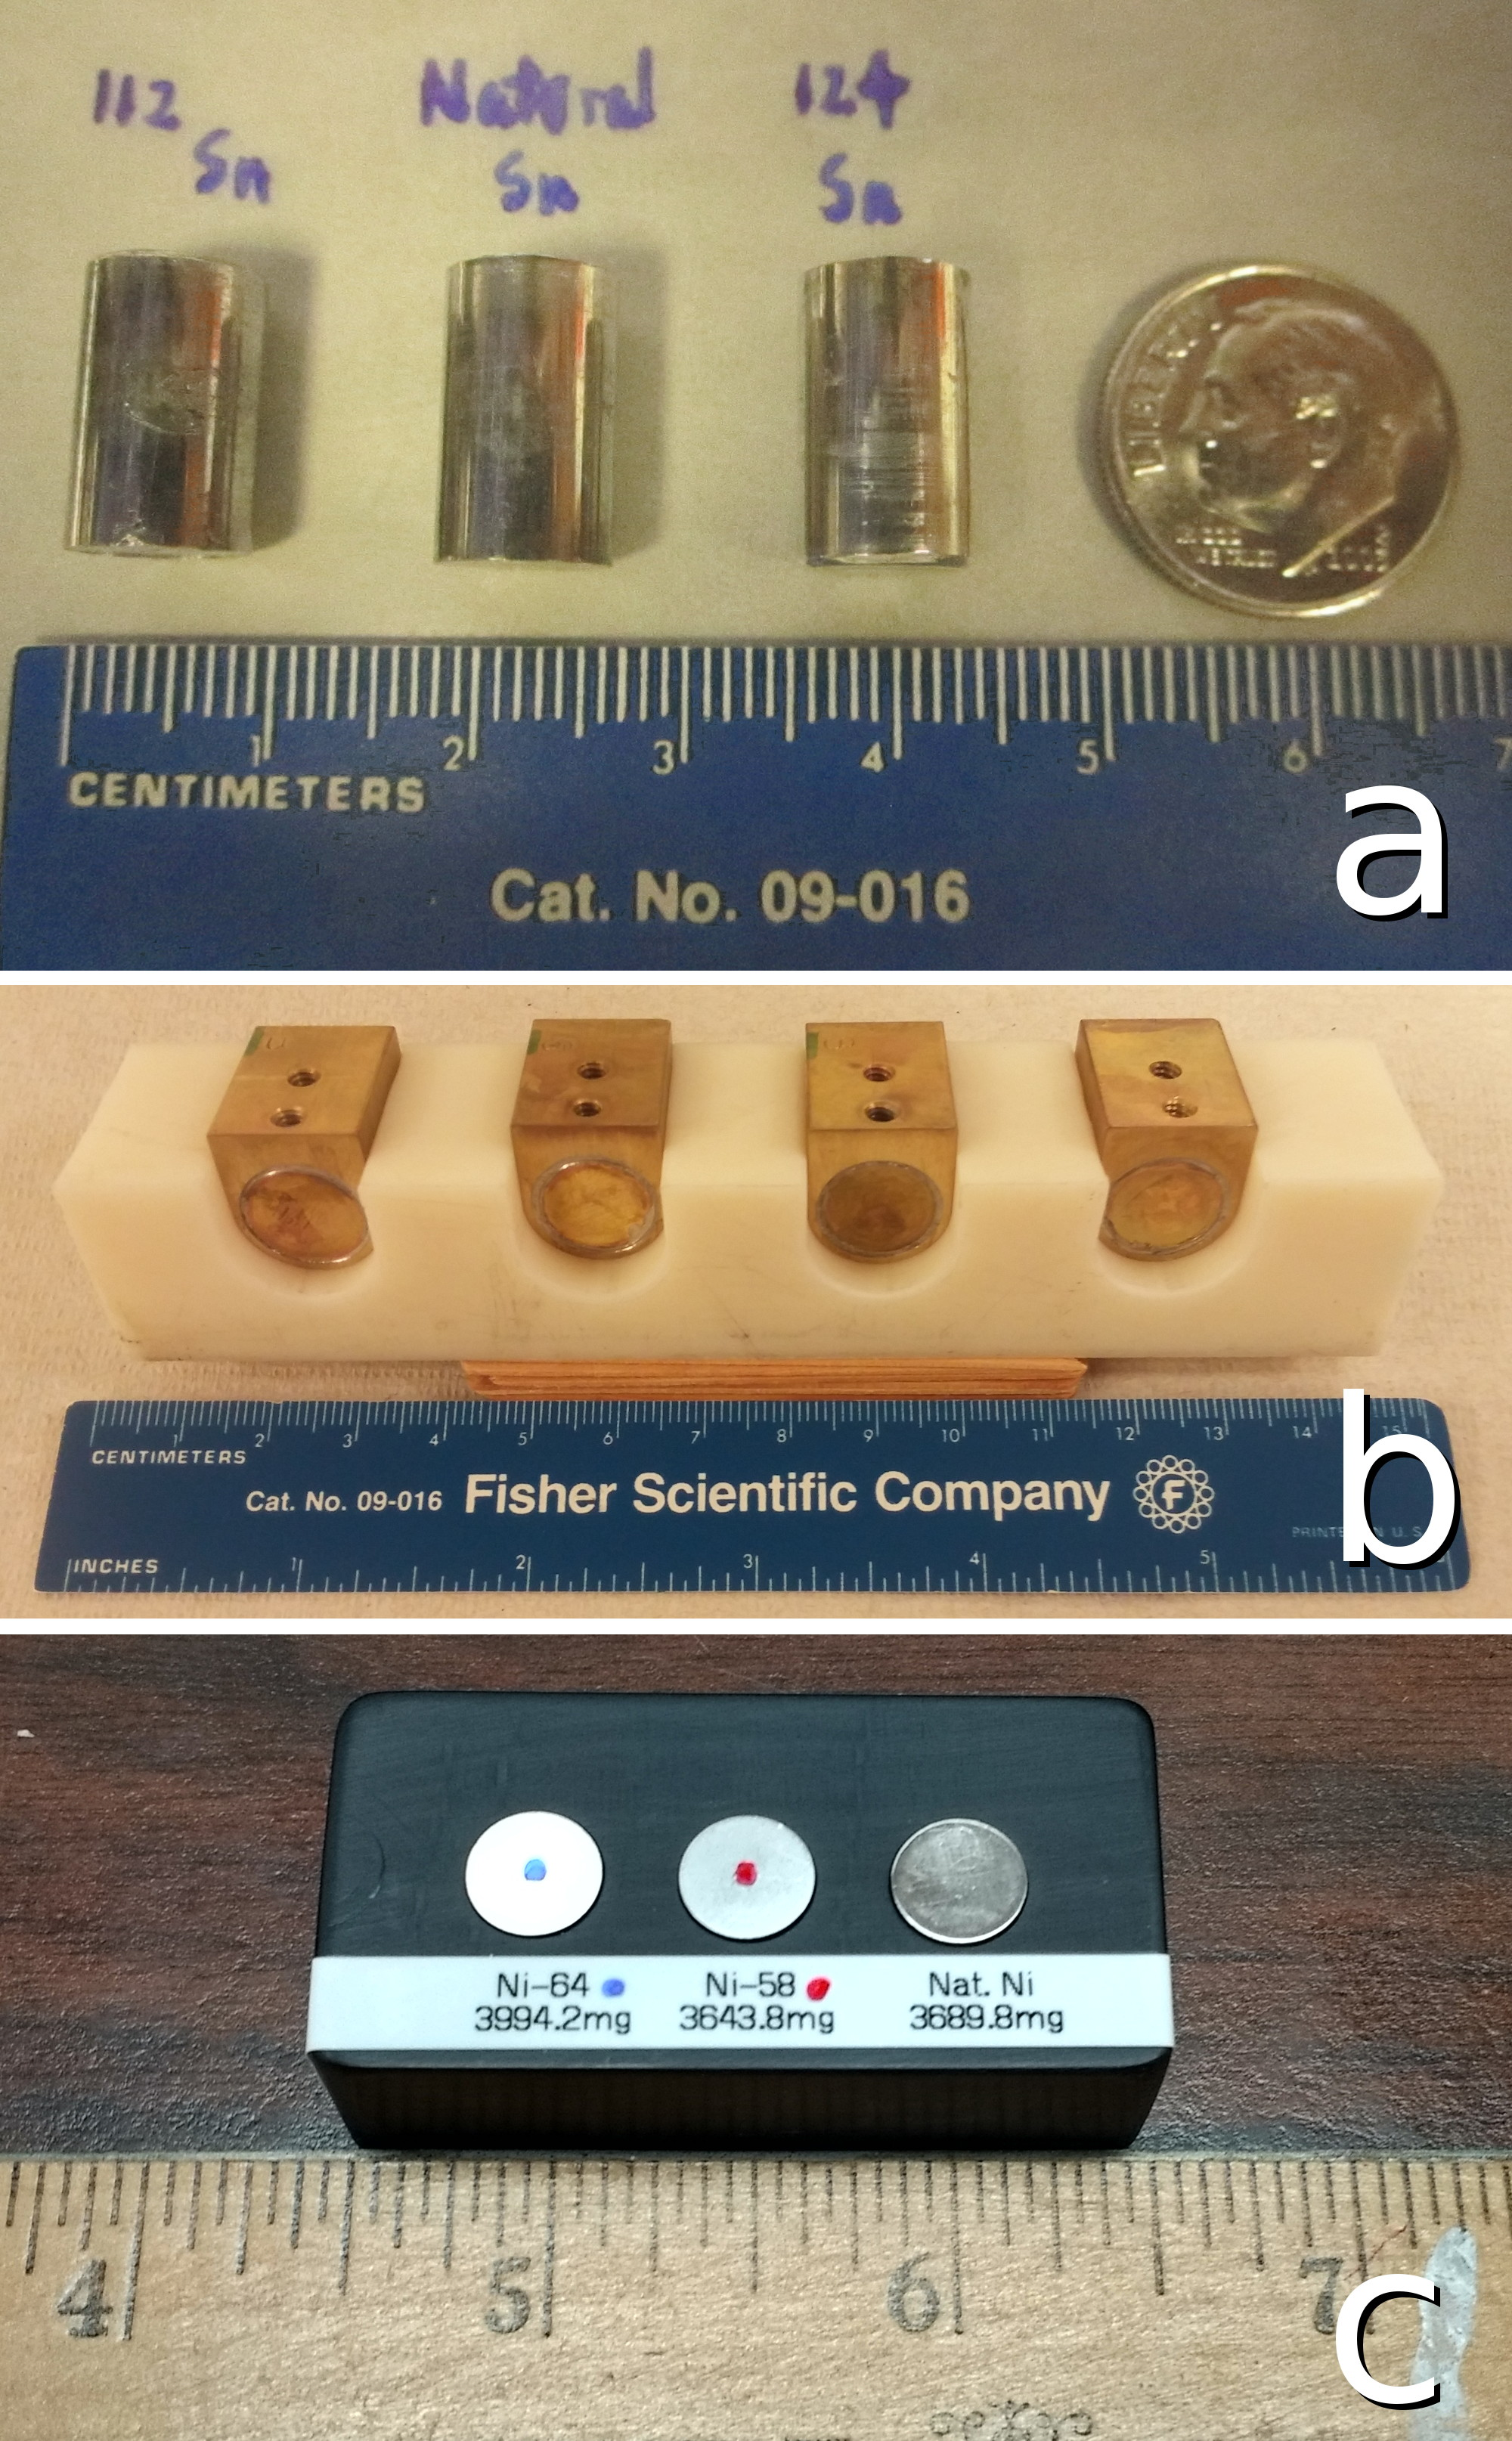
\includegraphics[width=0.3\textwidth]{figures/AllIsotopicSamples.jpg}
    \caption{(Color online) Section (a): the ${^{112,nat,124}}$Sn samples. Section (b): the 
        vessels used to hold water samples for the ${^{nat, 18}}$O \tot\  measurement. 
        Section (c): ${^{58,nat,64}}$Ni samples, shown end-on.}
    \label{SamplesImage}
\end{figure}

\section{Experimental Analysis}
The fundamental quantity of interest, \tot, is related to the flux
loss through a sample by:
\begin{equation}
I_{t} = I_{0}e^{-{\ell\rho\sigma_{tot}}}
\end{equation}
or, equivalently,
\begin{equation}
    \tot = -\frac{1}{\ell\rho}ln\left(\frac{I_{t}}{I_{0}}\right)
\end{equation}
where $I_{0}$ is the neutron flux entering the sample, $I_{t}$ is the neutron
flux transmitted through the sample without interaction, $\rho$ is the number
density of nuclei in the sample, and $\ell$ is the sample length. For thin
or low-density samples, flux attenuation through the sample will be small
(e.g., 13\% for our Ni samples at 100 MeV) and a large number
of counts will be required to determine the cross section to high
precision.

To identify valid neutron events and precisely determine the TOF start (micropulse start 
time) and TOF stop time (arrival at TOF detector) for each event, a series of corrections 
are required.  First, each event was assigned to the correct macropulse.
Time offsets accounting for cable and
electronics delay were applied, coarsely synchronizing all detectors with
facility-provided signals that indicated the proton micropulse arrival time.
To improve the time resolution for each TOF
event, the digitized waveform for each event was passed 
through an offline software constant-fraction discriminator (CFD) algorithm,
improving the precision of the arrival time at the TOF detector.
In addition, a $\gamma$-ray-averaging
procedure (cf. \cite{Shane2010}) was used to improve the precision of each
micropulse start time. After these corrections, the final TOF resolution
(taken as the FWHM of the $\gamma$-ray peak in the TOF spectra) ranged from
0.60-0.90 ns over the series of \tot\ measurements.
This is comparable to the resolution from 
our digitizer-mediated \tot\ measurement on Ca isotopes in 2008 \cite{Shane2010}.
For context, for a 100-MeV neutron and a TOF detector distance of 27 meters, a TOF 
uncertainty of 0.80 ns translates to an energy resolution of $\approx$900 keV.
For neutrons below $\approx$20 MeV, the TOF time resolution worsens because the traversal time 
through the 1-inch thickness of the TOF detector becomes non-negligible.
However, because the TOF of these neutrons is already very long (several hundred ns or
longer) the relative energy resolution ($\frac{\Delta E}{E}$) is
superior at low energies. As an example from one of our runs, a 5 MeV neutron with
a 0.82 ns detector-traversal time and an inherent TOF resolution of 0.80 ns
has an energy uncertainty of only 13 keV. These energy uncertainties
have been propagated through subsequent analysis into our \tot\ results below.

Calculating the neutron energy requires knowledge of the flight path
distance to high precision. We determined this distance by calculating 
putative \tot\ data for $^{\text{nat}}$C from 3-15 MeV from our measurement and 
comparing the resonance peaks in this region with high-precision literature data
sets. From this study, the TOF distance was determined as 2709 $\pm$1
\centi\meter\ for the Ni and Rh run configuration and 2554
$\pm$1 \centi\meter\ for the Sn and O run configuration.
\begin{figure}
    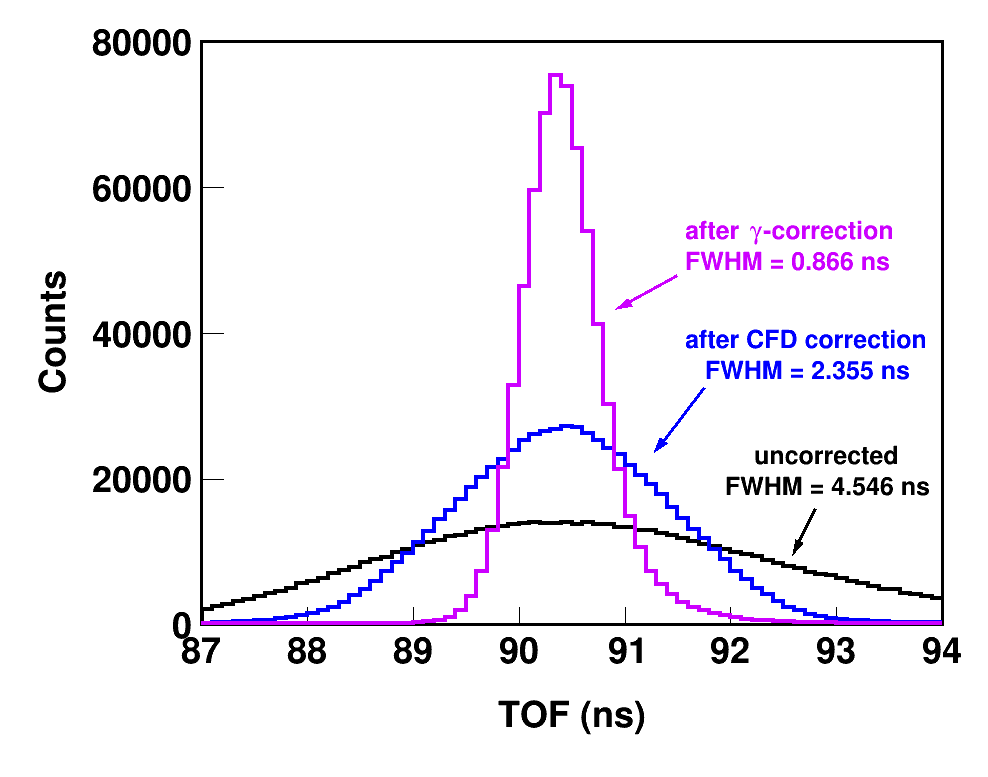
\includegraphics[width=\linewidth]{figures/TimeCorrections.png}
    \caption{(Color online) The effects of timing corrections on the $\gamma$-ray
        peak of a typical run are shown. The uncorrected spectrum is shown in black,
        the spectrum after correction with our software CFD is shown in blue,
        and the spectrum after correction with both our software CFD and
        $\gamma$-averaging is 
        shown in pink. For this run, the final $\gamma$-ray peak 
        FWHM after both corrections is 0.866 ns, comparable to the precision we
        achieved in our Ca study \cite{Shane2010}, which also employed $\gamma$-
        averaging.}
    \label{TimingCorrectionStudy}
\end{figure}

Before cross sections could be tabulated, the per-event deadtime had to be
modeled and corrected for. Because events are not processed
instantaneously, there is a brief period
after each trigger during which the digitizer is busy processing that trigger.
Any newly-arriving events in this period will be ignored,
privileging events arriving earlier and thus distorting
TOF spectra and resulting cross sections. This busy period is referred to as the
``analytic'' or ``per-event'' deadtime and can be corrected for according to standard 
techniques
\cite{Moore1980}. An additional complication is the possibility of flux
variation between micropulses. If there is no variation, the fraction of time
that the digitizer is dead for a given time bin $i$ can be calculated with a
simple formula, per Moore's analysis of rate-dependence of counting losses
\cite{Moore1980}:
\begin{equation}
    F_{i} = \sum^{N-1}_{j=0} R_{(i-j)\text{ mod N}}\times P_{j}
    \label{DeadtimeEquation}
\end{equation}
where $N$ is the number of time bins in the micropulse, $R_{x}$ is the rate of
detected events per micropulse in bin $x$, and $P_{j}$ is the probability that the
digitizer is still busy from a trigger $j$ bins ago.
Moore also provides a more advanced formula to generate the appropriate
dead-time correction in cases where the variation in beam flux 
is significant. However, an examination of our flux-per-micropulse data showed
very little flux variance across macropulses, except during the first 10\%
of the micropulses within each macropulse. To be conservative we discarded the
first 10\% of micropulses from each macropulse and used the simpler Eq.
(\ref{DeadtimeEquation}) to calculate the dead time fraction.

To model the experimentally-observed probability-dead, $P_{j}$, we
we fitted a logistic function to the observed spectrum for time
differences between consecutive events (see Fig.
\ref{TimeDifferenceBetweenEvents}). For a given bin $i$, the fraction of time that the 
digitizer is dead, $F_{i}$, is in essence a discrete convolution of the
\textit{measured} TOF spectrum with $P_{j}$. Note that except for the first and
last micropulses in a macropulse, all micropulses are consecutive, so deadtime effects can
``wrap around'' from the end of one micropulse to the next. For these wrap-around
contributions (that is, $j>i$), the (mod N) term ensures that the bin referred
to by $i-j$ is non-negative and has physical meaning as a time bin from the 
previous micropulse.
\begin{figure}
    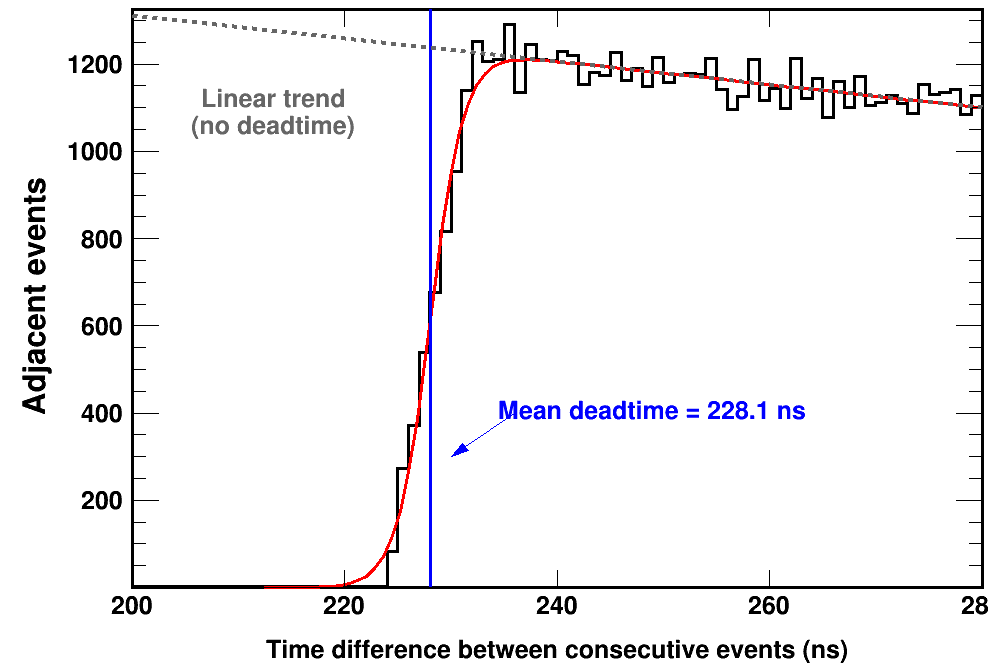
\includegraphics[width=\linewidth]{figures/TimeDifferenceBetweenEvents.png}
    \caption{(Color online) The time difference between adjacent TOF-detector
    events for a single run is plotted (black histogram). Below a certain
minimum time difference (the ``deadtime''), no events are recorded. A logistic
fit (red) models the detector's deadtime response and is used to generate a
deadtime correction. The underlying linearly-decreasing count rate (gray dashed
line) in incorporated into the logistic model. From the fit, a mean deadtime of
228.1 ns was extracted for the Sn and O run configurations (a similar
procedure was used to recover a deadtime of 159.7 ns for the Ni and Rh
run configurations).}
    \label{TimeDifferenceBetweenEvents}
\end{figure}

Because trigger processing is done in firmware onboard the digitizer,
the per-event deadtimes affecting our
measurement were reduced to between 150-230 \nano\second.
After we calculated the average probability-dead for each time bin,
the total number of events \textit{detected} in that bin, $N_{d}[i]$, could be
corrected to recover the \textit{true} number of events that would have been
detected in the absence of a per-event deadtime:
\begin{equation}
    N_{t}[i] = -ln\left[1-\frac{\frac{N_{d}[i]}{M}}{(1-F_{i})}\right]\times M
\end{equation}
where M is the total number of micropulse periods. At large TOFs (low energies) 
the correction is as low as a few percent,
but at small TOFs (high energies), the digitizer is often still dead
from the $\gamma$-ray flash and high-energy neutrons. In this regime
the correction can be quite large ($\approx$20\% for our Ni/Rh runs,
and $\approx$40\% for our Sn/O runs). The corrections needed for our measurement
are far lower than the typical analytic deadtime corrections required
with the deadtime mitigation scheme of previous analog measurements \cite{Finlay1993,
Abfalterer2001}.

In addition to analytic deadtime, there is an additional deadtime effect associated with 
digitizer readout to the data acquisition computer (DAQ). During data
collection, each pair of digitizer channels shares a common buffer for storing events.
After several seconds of acquisition, the digitizer begins readout at which time the
acquisition is paused and buffer contents are read out to the DAQ. However,
because each buffer is independently read out to the DAQ, it is possible that buffers
could be emptied and readied for new acquisition at slightly different times
(10-40 ms apart), and a mismatch could develop between the number of macropulses
seen on different channels. Such run-time interactions between the firmware and USB
traffic of the DAQ were difficult to characterize, but we estimate that they might cause a 
systematic error of a few tenths of one percent in the number of macropulses seen
by different channels, depending on the user-defined 
threshold and the buffer size. This effect could contribute to the discrepancy at the
highest energies ($>$100 MeV) between our results and past analog-enabled
measurements.

During analysis, it was noted that occasionally (1 in 400 macropulses), one or two 
adjacent macropulses would have an abnormally small number of events. The frequency
of these ``data dropouts'' was similar to the rate of
switching between DPP and waveform modes; we suspect it is related to edge
case behavior right before or after a mode switch. To mitigate this issue,
we threw out any macropulse that had less than 50\% of the average event rate in either the
flux monitor or TOF detector channel.

After applying these corrections, the veto and integrated charge gates were applied to 
all events and surviving events were populated into TOF spectra (see Fig.
\ref{ExampleTOFSpectrum}). Next, room background was subtracted (responsible for 0.1\% to 
1\% of event rate, depending on energy) and spectra were mapped to the energy domain.
\begin{figure}
    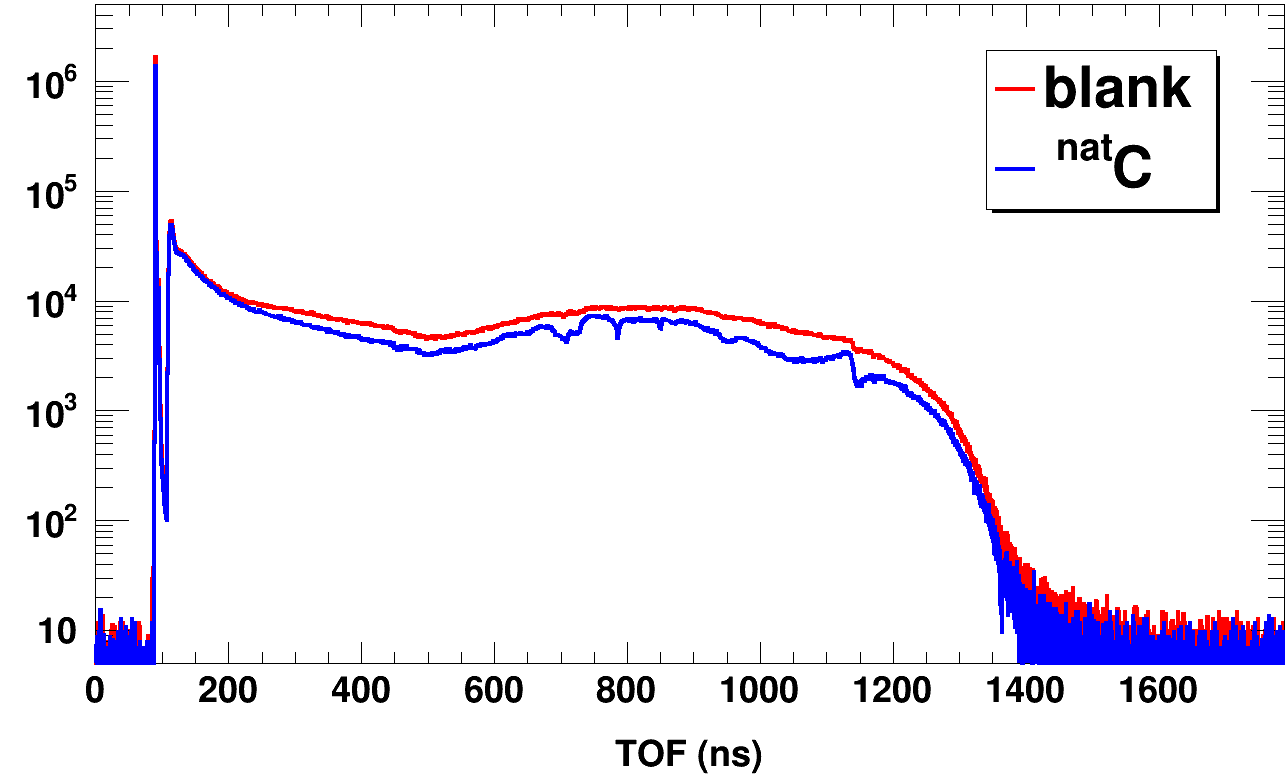
\includegraphics[width=\linewidth]{figures/exampleTOFSpectrum.png}
    \caption{(Color online) TOF spectra after analytic deadtime correction and
        veto and integrated charge gating for the blank sample (in
        red) and for the $^{\text{nat}}$C sample (in blue), from the Ni/Rh experiment.
        The $\gamma$-ray peak is visible as a sharp spike at 90 ns, followed by
        the highest-energy neutrons at 130 ns. The small spikes spaced 60 ns
        apart (visible before 90 ns and after 1500
        ns) are identified as $\gamma$-ray peaks from a low-level, continuous
        ``drip'' 
        of protons onto the tungsten target caused by mistuning of the proton 
        buncher; their effect on the calculated cross sections is negligible.
    }
    \label{ExampleTOFSpectrum}
\end{figure}

From these energy spectra, the raw cross sections were calculated, bin-wise, as follows:
$$
\tot = -\frac{1}{\ell\rho_{n}}
\ln \left(\frac{I_{0}}{I_{s}}\times\frac{M_{s}}{M_{0}}\right)
$$
where $\frac{I_{0}}{I_{s}}$ is the ratio of counts in the energy spectra between 
the blank and sample, $\frac{M_{s}}{M_{0}}$ is the ratio of counts in the
monitor detector between the sample and blank (for flux normalization), $\ell$ is the length 
of the sample, and $\rho_{n}$ is the number density of atoms in the sample.

Finally, two isotope-dependent corrections were applied to the raw cross
sections. First, because the blank sample contains air and not vacuum,
the cross section of air must be added to each sample's cross section.
For the sample most affected by this correction (Rh), this correction was 2 mb.
Second, the cross section for $^{64}$Ni was corrected for the isotopic enrichment of our
sample (92.2\%) using our measured $^{\text{nat}}$Ni cross section. All other isotopes were 
sufficiently pure such that the impurity correction was negligible.

To validate our analysis, we first benchmarked our \tot\ measurements of natural samples
($^{\text{nat}}$C, $^{\text{nat}}$Ni, $^{\text{nat}}$Sn, and
$^{\text{nat}}$Pb) against the high-precision data sets on natural samples from Finlay
\cite{Finlay1993} and Abfalterer \cite{Abfalterer2001}, shown in Fig.
\ref{LiteratureBenchmarking}. Our natural sample results
are in excellent agreement with 
these previous results from 3-100 MeV and show slight deviation above 100 MeV (a
relative difference of up to 5\% at 300 MeV), suggesting a small systematic
error at high energies in one or both approaches when the instantaneous neutron
flux is highest. As an additional diagnostic, we compared 
\tot\ results from our long and short natural carbon targets and
found excellent agreement, within 1\% throughout the measured energy domain.

Extracting the \oSixEight\ neutron \tot\ required subtraction of the
well-measured neutron \tot\ for H. To better characterize
the additional systematic uncertainty
associated with this subtractive analysis, we subtracted our measured
values for \oSix\ neutron \tot\ from our raw D$_{2}$O and H$_{2}$O data and 
calculated the D-to-H relative difference. A
comparison of our D-to-H relative difference with that of
\cite{Abfalterer1998} is shown in Fig. \ref{DtoH}.
\begin{figure}[tb]
    \centering
    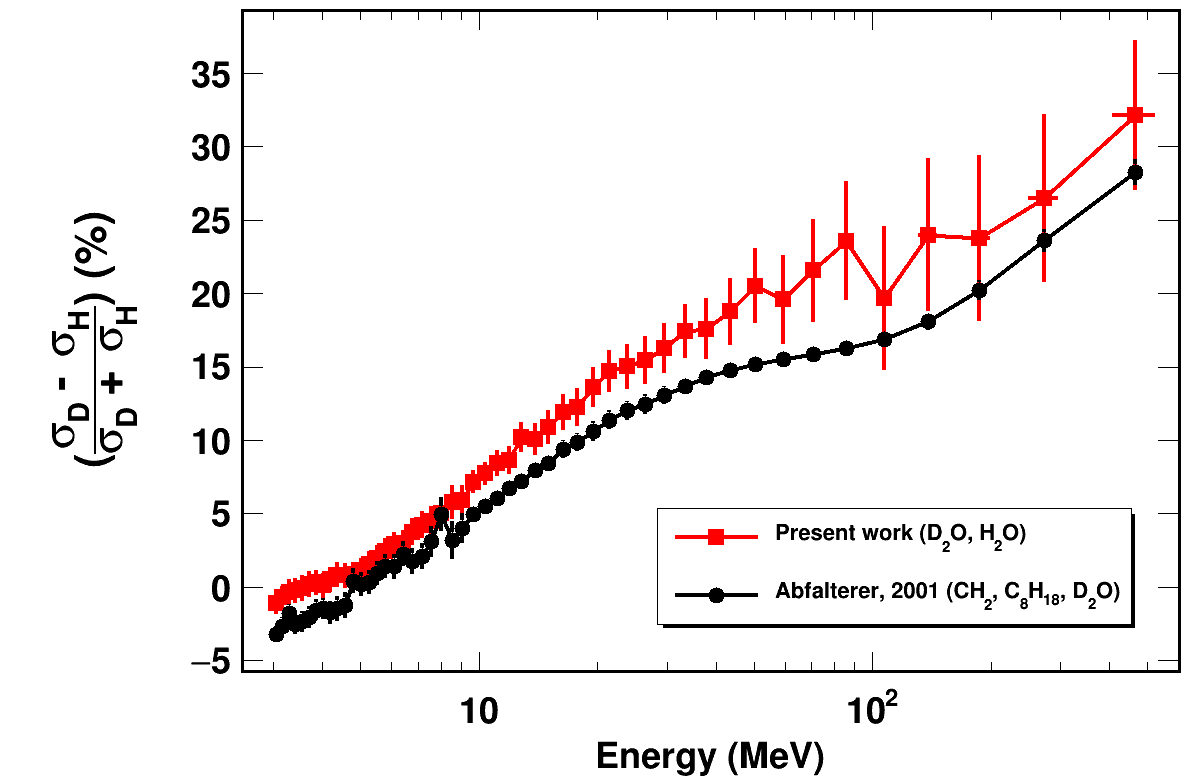
\includegraphics[width=\linewidth]{figures/relativeDiff_DtoH.png}
    \caption[\tot\ relative difference between deuterium and hydrogen from our measurement]
    {The \tot\ relative difference between deuterium and hydrogen,
        as calculated by subtraction of our O \tot\ results from
        D$_{2}$O and H$_{2}$O. Data from our measurement are shown as red
        squares; the data of Abfalterer et al. \cite{Abfalterer1998} are shown
    as black circles.}
    \label{DtoH}
\end{figure}
Our results differ systematically from the previous (analog) measurement by 2-3\% throughout the
energy range, comparable to the 2\% systematic difference between our final
\oSix\ neutron \tot\ results and those of \cite{Abfalterer2001}. The size and
uniformity of these systematic differences is consistent with
a combination of slight ($\approx$ 1\%) normalization errors
in some or all of the H, D, O, and C neutron \tot\ results,
both in our measurement and in the literature.
\begin{figure}
    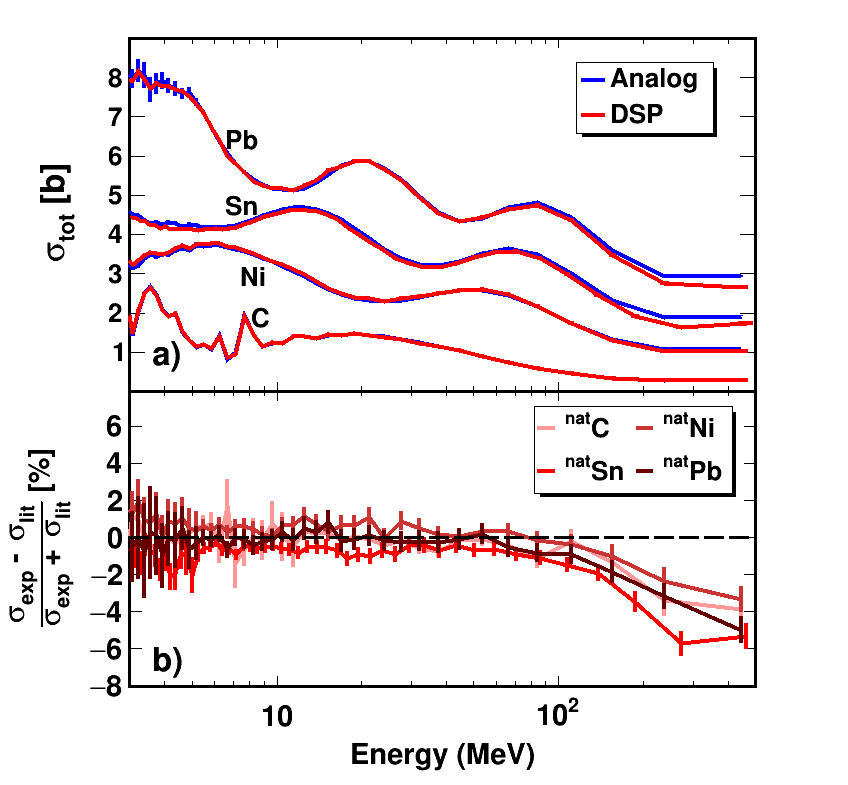
\includegraphics[width=\linewidth]{figures/literatureBenchmarking.png}
    \caption{(Color online) A comparison of literature data (taken with analog
    techniques) and our results (signals processed with a digitizer, or ``DSP'')
    for natural C, Ni, Sn, and Pb. In panel (a), the absolute cross sections are shown from
    3-500 MeV; in panel (b), the relative differences between the literature data and
    our data are shown in percent. From 3-100 MeV, our data are fully consistent with the
    literature datasets but above 100 MeV, a difference arises, peaking at
    $\approx$5\% at 300 MeV.
b}
    \label{LiteratureBenchmarking}
\end{figure}

\section{Experimental Results}
Our absolute \tot\ results for O, Ni, and Sn isotopic targets are shown in Fig.
\ref{SixPanel} (results for Rh are shown in the supplemental materials).
Literature isotopic \tot\ measurements
(where they exist) are shown alongside our results for comparison.
Residuals between our data and any existing literature data are also shown.
In each figure, the literature data sets have rebinned to match the bin
structure of our data to facilitate comparison. In regions with a low density of
states where individual resonances are visible (e.g., $^{\text{nat}}$C
below 10 MeV), this rebinning washes out the fine structure of the
cross section data.

Except for the already well-measured \oSix, our new data significantly
extend knowledge of the neutron \tot\ for each sample. In the case of \oEight,
\niEight, \rhThree, and \snFour, almost no previous data were available
above 20 MeV. Our new data are in reasonable agreement with the previous
measurements where available. In the cases of the rare isotopes \niFour\ and \snTwelve,
data were available at only one energy, 14.1 MeV, from a study from more than 50
years ago \cite{Dukarevich1967} and our present values are in excellent agreement, within 2-3\%.

Our results for relative differences between isotopic pairs \oSixEight,
\niEightFour, and \snTwelveFour\ are shown in Fig. \ref{ThreePanelRelDiff}. In
\oSixEight, the purely-isoscalar SAS model grossly reproduces the relative
difference below 100 MeV, but fails completely above 100 MeV. Near 200
MeV, the \oEight\ \tot\ drops below that of \oSix\ resulting in a negative
relative difference, in keeping with the Ramsauer-logic expectation of Eq.
(\ref{OscillatoryModel}) that \tot\ oscillation minima shift to higher
energies as A is increased. In the relative difference subfigures for 
\niEightFour\ and \snTwelveFour, the average \tot\ values are below the
SAS model trend ($r \propto A^{\frac{1}{3}}$), shown by the black dashed lines. 
The well-known $r \propto A^{\frac{1}{6}}$ trend in Sn isotope shift data 
\cite{Anselment1986} are also shown for reference and
underpredict the relative differences. As was noted by Dietrich et al. in
their study of \tot\ relative differences in W isotopes, a simultaneous optical
model analysis along the entire isotopic chain (a l\'a \cite{Mueller2011})
may be required to reproduce the oscillatory behavior seen in the relative differences.
The individual Dispersive Optical Model fits to \oSixEight, \niEightFour, and
\snTwelveFour\ in the following section lay the groundwork for a future study of
this type.
\begin{figure*}[tb]
    \centering
    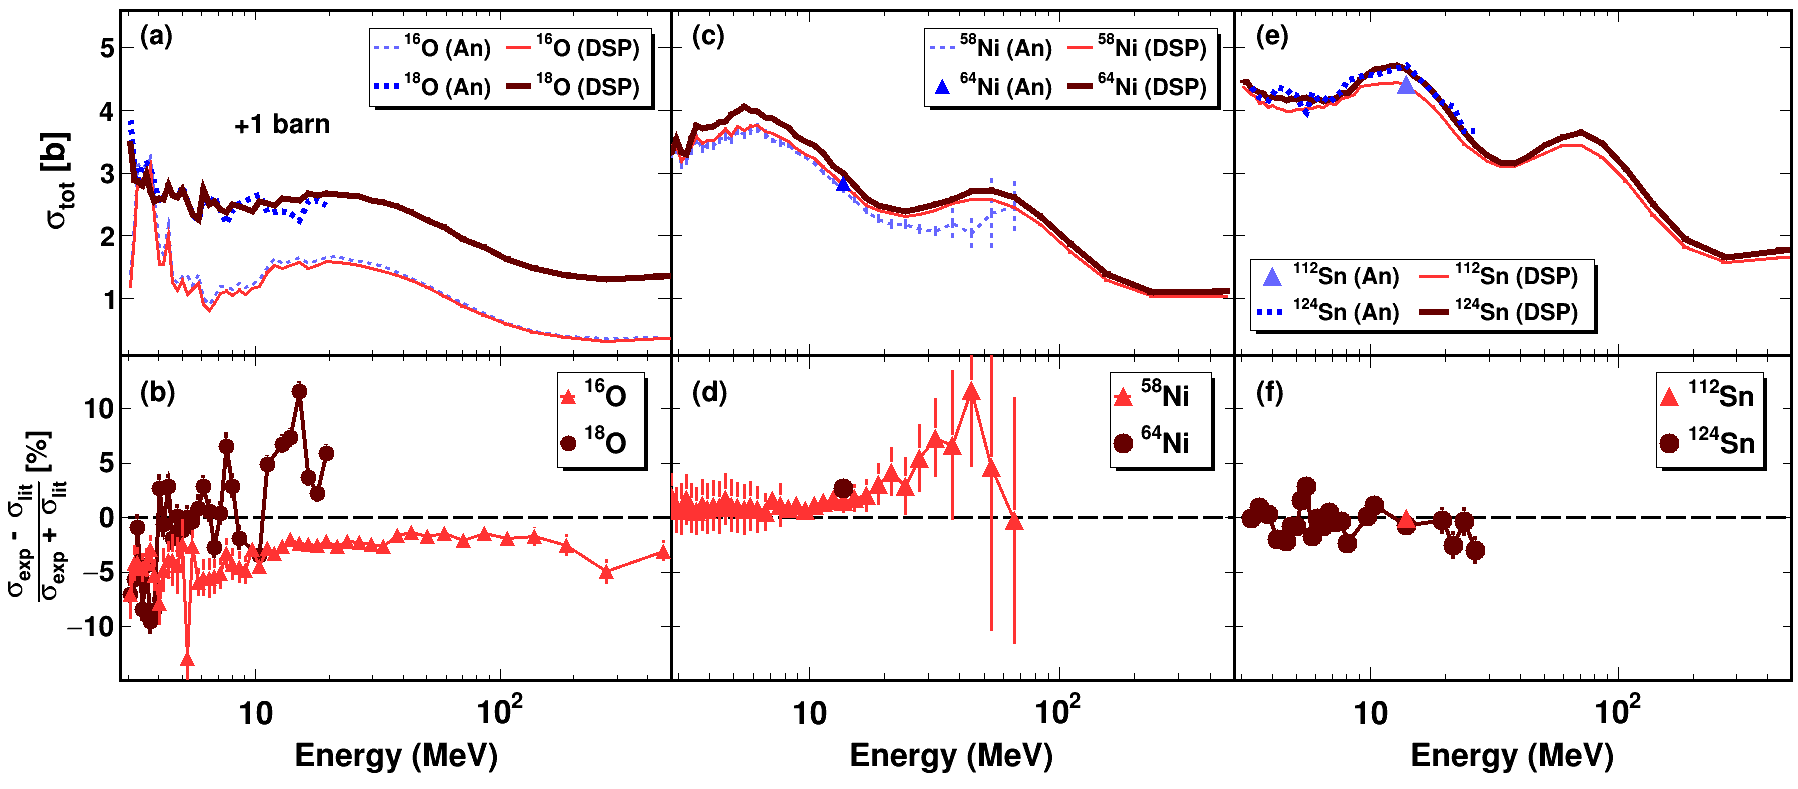
\includegraphics[width=\textwidth]{figures/SixPanel.png}
    \caption[Neutron \tot\ for \oSixEight, \niEightFour, and \snTwelveFour: our results and literature data]
    {(Color online) Neutron \tot\ for \oSixEight, \niEightFour, and \snTwelveFour: our results 
        and literature data.  In the upper three panels, our digitizer-measured
        isotopic results are shown in red and
        corresponding analog-measured literature data \cite{Finlay1993, 
        Perey1972, Vaughn1965, Salisbury1965, Perey1993, Dukarevich1967,
        Harper1982, Timokhov1989, Rapaport1980} are shown in blue.
        The data for \oEight\ in panel a) have been
        shifted up by 1 barn for visibility.
        The lower three panels show residuals between our data and the
        literature data shown in the upper three panels.
    }
    \label{SixPanel}
\end{figure*}
\begin{figure*}[tb]
    \centering
    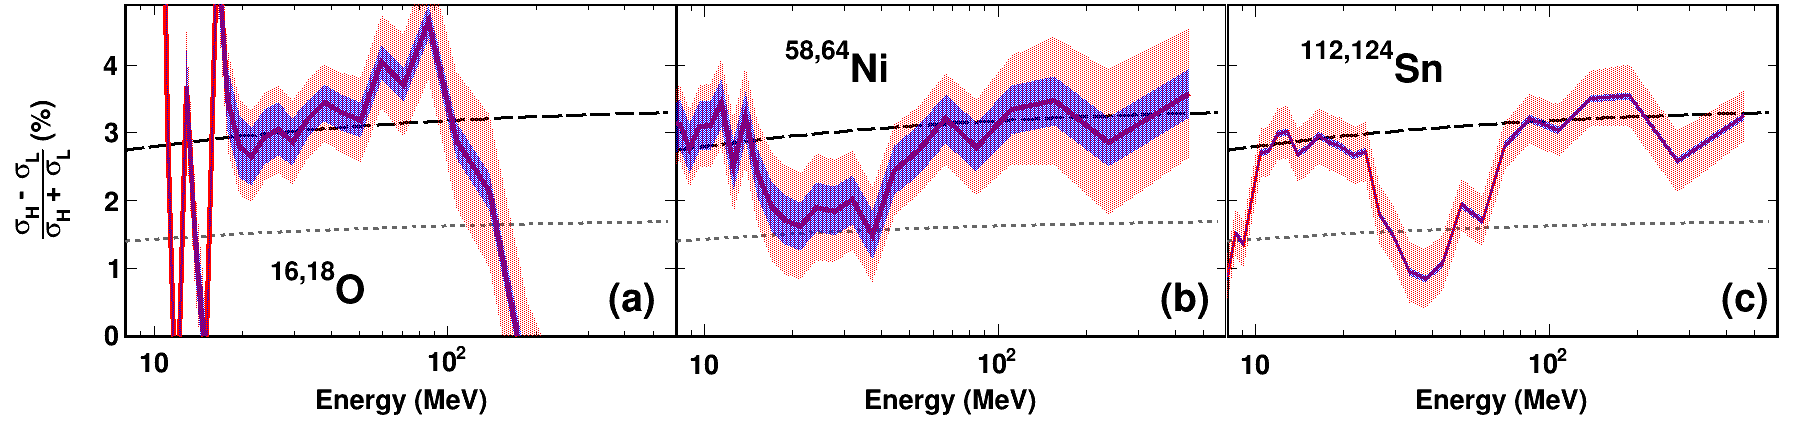
\includegraphics[width=\textwidth]{figures/ThreePanelRelDiff.png}
    \caption[\oSixEight, \niEightFour, \snTwelveFour\ neutron \tot\ relative difference]
    {
        (Color online) \oSixEight, \niEightFour, \snTwelveFour\ neutron \tot\ relative differences
        from our measurement. In each figure, the black dashed line shows the 
        prediction for the \tot\ relative difference per the strongly-absorbing 
        sphere (SAS) model of Eq. (\ref{SASAbsolute}), which assumes a simple 
        A$^{\frac{1}{3}}$ size scaling for the nuclear radius.
        The gray dotted line shows the
        SAS model prediction but with an
        A$^{\frac{1}{6}}$ size scaling. The blue band in each panel indicates
        uncertainty due to target thickness imprecision;
        the red band in each panel
        indicates uncertainty from both target thickness and statistics.
    }
    \label{ThreePanelRelDiff}
\end{figure*}

\section{DOM Analysis}
The Dispersive Optical Model (DOM) is a phenomenological Green's-function
framework enabling a simultaneous and self-consistent analysis of nuclear
structure and reaction data. An essential feature of the DOM is the enforcement of a dispersion
relation between the complex components of the self-energy across the entire
energy domain, allowing structural data from below the Fermi energy
(e.g., charge densities, bound levels) to constrain the potential above,
and data from above the Fermi energy (e.g., elastic, reaction, and total
cross sections) to constrain the potential
below. Using our new \tot\ data for \oSixEight, \niEightFour, and \snTwelveFour, we
performed a comprehensive DOM analysis on these isotopes and also
\caAughtEight\ and \pbEight. Compared to previous DOM
analyses \cite{Mueller2011, Atkinson2017, Mahzoon2014, Mahzoon2017},
we employ an updated version of the DOM that has been generalized for use with
any even-even nucleus that is not too deformed. Partial filling of open shells,
as for the neutron \dFive\ valence shell in \oEight, is accommodated with a simple
pairing parameter $\Delta$ (see \cite{PruittPhDThesis}). The other major
methodological difference is our use of Markov-Chain Monte Carlo (MCMC) for
parameter optimization, discussed below. 

In this work, we give the functional forms used to define the
potential (Appendix \ref{DOMFunctionalForms}), optimized parameter values with
uncertainties (Appendix \ref{DOMParameterValues}), and figures showing the quality
of the DOM reproduction of experimental data (Appendix \ref{DOMFitResults}).
For additional details on the underlying DOM formalism, see \cite{Mahaux1991,
Dickhoff2018}. Except where indicated, the corpus of experimental data used for
fitting is the same as in \cite{PruittPhDThesis}. To situate the reader, we discuss the
experimental data and DOM results for \oSixEight\ in full detail. The
experimental data used and fit quality for \caAughtEight, \niEightFour,
\snTwelveFour, and \pbEight\ are similar and key differences are noted.

\subsection{\oSix\ experimental data used in DOM analysis}
For protons, twenty-eight differential elastic cross
sections data sets and twenty analyzing power data sets from 10-200 MeV were
incorporated. Only three proton reaction cross section data sets, ranging from 20-65 MeV,
were available. As an added constraint, we used systematic trends
from the comprehensive review of Carlson \cite{Carlson1975} to generate proton
reaction cross section pseudo-data from 70-200 MeV, which were included in the fit.
For neutrons, ten differential elastic cross section
data sets from a 10 MeV to 95 MeV, a single
neutron reaction cross section data point at 14 MeV, and our newly-measured \tot\ results
for $^{16}$O were included. In all, over sixty experimental nucleon scattering
data sets were used to constrain the \oSix\ parameters.

In addition to nucleon scattering data, several sectors of bound-state data were
included in the fit. Neutron (proton) 0\pOne\ and 0\dFive\
single-particle level energies were
assigned according to the nucleon separation energies of $^{16}$O and
$^{17}$O isotopes ($^{16}$O, $^{17}$F isotopes) \cite{AME2016}.
Charge density distributions were taken from the compilation \cite{DeVries1987}.
Since the time of that compilation,
new experiments (particularly muonic atom measurements) have improved the precision
of many root-mean-square (RMS) charge radii by roughly an order of magnitude \cite{Angeli2013}.
To account for these improved data, we rescaled the distributions from
\cite{DeVries1987} to recover the updated
RMS charge radii while still conserving particle number. We also fitted directly
to the updated RMS charge radii of \cite{Angeli2013}.
Because the DOM self-energy does not necessarily conserve particle number, we
included the ``experimental'' proton and neutron numbers of 8 as part of the
fit. Lastly, the total binding energy of \oSix\ from \cite{AME2016} was
included as a constraint. 

\subsection{\oEight\ experimental data used in DOM analysis}
A large corpus of proton elastic scattering data for \oEight\ was
available from the EXFOR database. Twenty-eight proton elastic differential cross
sections were included with an energy range from 10-200 MeV in the lab frame.
Unfortunately, no proton reaction cross section data were available at all in
the relevant range of 10-200 MeV. As with \oSix, we generated proton reaction cross section pseudo-data from
systematic trends in \cite{Carlson1975} from 70-200 MeV. On the neutron side, two
differential elastic cross section data sets were included, at 14 and 24 MeV,
but no analyzing powers were available. One datum for the neutron reaction cross
section, at 14.1 MeV, was incorporated as well.
Our \tot\ results for \oEight\ were the
sole neutron total cross section data used in the fit. The energies of the
proton and neutron 0\pOne\ and 0\dFive\ single-particle
levels were assigned according to the same procedure used for \oSix.

Unlike \oSix, for \oEight, no charge density distribution was available from
\cite{DeVries1987}. To approximate it, we rescaled the charge density
distribution used for \oSix\ to give the \oEight\ RMS charge radius of
\cite{Angeli2013} while preserving 8 units of charge.
As with \oSix, we also fitted to the
RMS charge radius directly and to the particle numbers N and Z and the
total binding energy.

\subsection{MCMC analysis}
Optimization of non-local DOM potentials is not a trivial computational task.
For example, the \caEight\ analysis of \cite{Mahzoon2017} involved a joint
optimization of over 60 highly-correlated parameters, many newly introduced, to
accommodate the available experimental data. The potential is
often severely underconstrained and multiple reasonable optima are expected.
In such a space, traditional gradient-descent methods often fail to find optima
or are hopelessly slow. Even if a reasonable optimum is found, robust
uncertainty analysis requires information about the region around the optimum and
accounting of inherent model errors.

To fulfill these requirements, we used the affine-invariant, ensemble-sampling
MCMC utility emcee \cite{Foreman-Mackey2013} based on the work of \cite{Goodman2010}. For an
accessible introduction to Bayesian data analysis and applied MCMC, see
\cite{Sharma2017}. Computations were performed using the facilities of the Washington University
Center for High Performance Computing, which were partially provided through NIH
grant S10 OD018091. In the ensemble-sampling approach, several hundred
``walkers'' are first randomly initialized in parameter space for each nucleus according to a
uniform prior distribution. At each subsequent step $t$ during the
random walk, each walker's position is updated from $\vec{x_{t}} \rightarrow
\vec{x_{t+1}}$ either by accepting a new position $\vec{x'}$ with probability:
\begin{equation}\label{AcceptanceEquation}
    p(\vec{x}\rightarrow \vec{x'}) = \min(1,\frac{U(\vec{x'}|D)}{U(\vec{x}|D)}).
\end{equation}
or by remaining in the same position $\vec{x}$ with probability
$1-p(\vec{x}\rightarrow \vec{x'})$. New positions are proposed according
to the stretch-move proposal distribution of \cite{Goodman2010} (for our stretch
move scaling, we used $\alpha = 1.3$ to improve the acceptance fraction from
roughly 0.05 to 0.15). In Eq.
(\ref{AcceptanceEquation}), the utility of a parameter vector conditional on the
experimental data $U(\vec{x}|D)$ was defined according to Bayes rule
\begin{equation}
    U(\vec{x}|D) \propto L(D|\vec{x}) \times P(\vec{x}),
\end{equation}
in terms of a likelihood function and a prior distribution. The likelihood
function was taken as a weighted least-squares function where each datum was assigned
a weight and a model error:
\begin{equation} \label{LikelihoodFunction}
    L(D|\vec{x}) = \sum_{d=1}^{N_{d}} w_{d} \frac{1}{N_{i}} \sum_{i=1}^{N_{i}}
    \left(\frac{y^{calc}_{d,i}-y^{exp}_{d,i}}{\sigma^{calc}_{d,i}+\sigma^{exp_{d,i}}}\right),
\end{equation}
where
\begin{itemize}
    \item $N_{d}$ is the number of different sectors of available experimental
        data, $D$ (e.g., proton \el\ cross sections,
binding energy, etc.),
    \item $w_{d}$ is a scalar weight assigned to the entire sector $d$,
    \item $N_{i}$ is the number of data points in a sector $d$,
    \item $y^{calc, exp}_{d,i}$ are the calculated and experimental values,
        respectively, for the $i$th datum of sector $d$,
    \item $\sigma^{calc, exp}_{d,i}$ are the calculated and experimental errors,
        respectively, for the $i$th datum of sector $d$,
    \item $w_{d,i}$ is a scalar weight assigned to the $i$th datum
        $y_{d,i}$ of data sector $d$.
\end{itemize}

Due the only approximate value
of any optical potential for realizing the true many-body 
potential, it should be expected that DOM predictions for nuclear observables
will suffer from some degree of error inherent to the model. For example, previous
OM analyses tend to easily reproduce low-angle experimental \el\ data taken at
lower scattering energies but are increasingly discrepant at high energies
and at backward angles, where the predicted cross sections may
differ from experimental results by an order of magnitude or more. 

Neglecting model discrepancy may
dramatically bias fitted parameters and underestimate variances of extracted
quantities. Table \ref{ModelDiscrepancyTable} shows the model discrepancy terms we used 
for each data sector. The choice of model discrepancy for each point
is depends on several factors, including the functional form chosen for the
potential, numerical truncations, and the plausible range of the nuclear datum being 
calculated. In the final analysis, we settled on discrepancy terms based
on how well preliminary fits could reproduce differing regions of each data sector
coupled with intuition from the successes and failures of past optical model analyses.
In principle, the form of these model discrepancy terms should also be treated as random
variables, but due to computational limitations and the already-challenging size
of the DOM parameter space, we elected to fix the model discrepancy terms.

\begin{table}[tb]
    \centering
    \bgroup
    \def\arraystretch{1.8}%
    \begin{tabular}{ c c c c }
        \el\ & A & \tot\ & \rxn \\
        \hline
        \textcolor{red}{0.25} $\%/\degree_{CM}$ & \textcolor{red}{0.10}
            & \textcolor{red}{0.25}\% & \textcolor{red}{0.25}\% \\
    \end{tabular}
    \begin{tabular}{ c c c c c }
        $\epsilon_{nlj}$ & BE/A & N,Z & $r_{rms}$ & $\rho_{Q}$ \\
        \hline
        \textcolor{red}{0.10} MeV & \textcolor{red}{5}\% & \textcolor{red}{0.10}
        & \textcolor{red}{0.005} fm & \textcolor{red}{1}\%\\
    \end{tabular}
    \egroup
    \caption{Model discrepancy terms for each data sector used in
        MCMC utility function. For \el\, the model discrepancy was defined to
        increase linearly with respect to the scattering angle in the
        center-of-mass frame, with units of \% per degree. $\epsilon_{nlj}$
        are the single-particle energies for valence nucleons as calculated
        from separation energies in \cite{AME2016},
        $r_{rms}$ is the root-mean-square charge radius, and
    $\rho_{Q}$ is the charge density distribution.}
    \label{ModelDiscrepancyTable}
\end{table}

The prior distribution $P(\vec{x})$ was taken to be uniform over a
physically-reasonable range for each parameter. For example, the
diffusenesses of all Woods-Saxon terms were restricted to 0.4-1.0 fm.
After $N$ samples have been taken from the posterior distribution,
a subset can be used to estimate the true parameter distributions,
and physics results calculated for each sample. Guaranteeing that this subset is
representative of the true distribution is one of the most challenging aspects
of MCMC analysis and is discussed in the next section. Appendix A
shows the parameter definitions and prior distributions used in the present
analysis.

Following \cite{Foreman-Mackey2013} we attempted an
autocorrelation analysis to test for convergence
and estimate the number of independent samples we had collected for each nucleus.
For $N$ total samples collected of a quantity $f$ over the probability density
$p(\theta)$, the normalized autocorrelation function is
\begin{equation}
    \hat{\rho}_{f}(\tau) = \frac{\hat{c}_{f}(\tau)}{\hat{c}_{f}(0)}
\end{equation}
where
\begin{equation}
    \hat{c}_{f}(\tau) = \frac{1}{N-\tau} \sum_{n=1}^{N-\tau}
    (f_{n}-\mu_{f})(f_{n+\tau}-\mu_{f}).
\end{equation}
Here $f_{n}$ is the $n^{th}$ sample of $f$ and $mu_{f}$ is the mean value of
$f$. By definition, $\hat{\rho}_{f}(0) = 1$. At small $\tau$, $f_{\tau}$ will still
be strongly correlated with $f_{0}$, so $\hat{\rho}_{f}(\tau)$ will be close to
1. At large $\tau$, $f$ will ``forget'' where it started and $f_{\tau}$ will
decay toward 0. With $\hat{\rho}_{f}(\tau)$ in hand the integrated autocorrelation
time can be computed
\begin{equation}\label{TauEstimator}
    \tau_{f} \equiv \sum_{\tau=-\infty}^{\infty} \hat{\rho}_{f}(\tau) \approx
    1 + 2 \sum_{\tau=1}^{M} \hat{\rho}_{f}(\tau),
\end{equation}
where $M << N$, then used to estimate the variance of $f$ over $p(\theta)$:
\begin{equation}\label{VarianceEstimator}
    \sigma^{2} = \frac{\tau_{f}}{N}\sigma^{2}_{p(\theta)}[f(\theta)]
\end{equation}
The number of independent samples is not $N$ but instead
$N/\tau_{f}$. For the approximation of Eq. (\ref{TauEstimator}) to
converge, $M$ must be several times larger $\tau_{f}$. Thus, a reasonable
estimate of $\tau_{f}$ requires a very large number of samples, say, $N > 100\tau_{f}$.

In an ideal MCMC analysis, $\tau_{f}$ could be computed for all $f$ of
interest (each parameter and extracted physics quantity) and Eq.
(\ref{VarianceEstimator}) would give the complete variance, including sampling
error from MCMC. In practice, we found this to be computationally infeasible
for the DOM parameter space. For example, in our analysis of \oEight, we were
able to perform $N=31000$ steps for each of 336 walkers (more than 100,000
CPU-hours in total). Over this domain, we calculated the
integrated autocorrelation time, $\tau_{p}$, for each potential parameter $p$,
was roughly 2800 -- that is, $N \approx 11\tau_{p}$, rather than the
$N > 100\tau_{p}$ rule-of-thumb condition for convergence of the $\tau$ estimate
for each parameter. Similarly, calculating $\tau_{f}$ for other quantities
of interest (such as the neutron skin of \oEight) was deemed unrealistic, given
our computational resources. We note that $\tau_{f}$ \textit{could} be considerably
smaller than $\tau_{p}$ due to the highly-correlated nature of DOM parameter space.

To proceed, we applied several commonsense tests to
judge whether our parameter and extracted-quantity estimates were accurate.
First, we sampled as long as possible and used as many parallel walkers as
possible, given our computational resources. From time to time during sampling,
we analyzed the the mean walker positions and the mean walker position likelihood
as a function of sampling step. Encouragingly, for all nuclei walkers quickly
converged on a common region (within 1000 samples) and their mean parameter
values stabilized soon afterward (within 10000 samples), suggesting that walkers
were sampling a reasonably-optimal subspace. At this point, we considered the chain
tentatively converged. As an additional test, we re-started sampling from a different
(uniformly-random) initial position for each nucleus and found that a similar
optimal subspace was reached, again within roughly 1000 samples, indicating that
our results are independent of the initial walker positions. Finally, for a
``converged'' chain, we calculated extracted physics quantities (e.g., neutron
skins, scattering cross sections) for all walker at several intervals
to confirm that their mean values were stable. Again using \oSix\ and \oEight\ as
an example, we found their mean neutron skin values varied by less
than 0.001 and 0.01 fm, respectively, over several thousand sampling steps.
To be conservative (and given our expectation of very large autocorrelation times)
we used only the terminal sample for each walker chain to produce
the results presented here and in the companion paper \cite{Pruitt2020PRL}.
In the end, we expect that additional sampling would slightly
reduce the estimated variance of each extracted quantity but have a negligible
effect on the mean values. The estimated mean values and variances for each
parameter for each nucleus are listed in Appendix \ref{ParameterValues}.

\subsection{Fit results on $^{16}$O}
Figs. \ref{DOM_o16_scattering} and \ref{DOM_o16_structural} in Appendix
\ref{DOMFitResults} show the DOM fit of \oSix\ to experimental data via
MCMC sampling. The experimental proton \rxn\, neutron \el, \tot, 
and \rxn\, charge density distribution, RMS charge radius, binding energy per nucleon,
and \pOne\ and \dFive\ single-particle energy data are all well-reproduced,
suggesting that the DOM is a effect tool for modeling nuclei as light as A=16.
Almost all experimental proton \el\ data are recovered by the DOM
calculations with the exception of the location and magnitude of the diffraction
minima at backward angles, a regime known to be challenging from past
optical model analyses. To reproduce the \oSix\ proton \rxn\
pseudo-data, generated from \cite{Carlson1975}, a large volume imaginary term
was required above 100 MeV, which in turn reduced the spectroscopic strength in
the valence $\pi$ and $\nu$ \pOne\ shell by roughly 0.05. This connection
between large proton \rxn\ at high energies and modest reduction of valence
spectroscopic factors appeared on all isotopes we analyzed, indicating that a
non-negligible fraction of spectral strength rests above 100 MeV. We also note
the importance of the charge density distribution for determining the 
magnitude of the imaginary strength below the Fermi energy. For example, in test
fits where the charge density was not included as a constraint, most of the
negative imaginary strength was concentrated in the negative surface term
between $-30 E < \epsilon_{F}$ MeV, and the tail of the charge density was
overpredicted. With the charge density included as a constraint,
the negative surface term shrank by a factor of two and the negative volume term
grew to compensate, pushing nucleon density deeper in energy space and
increasing the binding energy closer to the experimental value. While
the proton \rxn, neutron \tot, and charge density appear to provide the most
stringent constraints on the self-energy out of all the data sectors we
considered, all sectors provided complementary information that is not fully
captured by any other sector.

The analyzing powers appear to be the most difficult sector of experimental data to
reproduce, with moderate deviations visible from 10-15 MeV for both protons and
neutrons and above 100 MeV for protons (see panels B and D of
Fig. \ref{DOM_o16_scattering}). Some
of the difficulty with the analyzing powers is attributable to our neglecting of
an imaginary spin-orbit term in the DOM potential used in this work, a choice
made due to the unreasonable unbounded growth of the imaginary spin-orbit term
as $\ell$ grows in the traditional $\ell\cdot\sigma$ definition used in
\cite{KoningDelaroche}. In a future analysis we intend to quantitatively
investigate the importance of the imaginary spin-orbit term and to compare
different options for its functional form.

\subsection{Fit results on $^{18}$O}
Figs. \ref{DOM_o18_scattering} and \ref{DOM_o18_structural} in Appendix
\ref{DOMFitResults} show the DOM fit of \oEight\ and \oEight\ experimental data
used as a constraint. Of the systems we studied, \oEight\ was one of most challenging due to the 
paucity of experimental data. To constrain the negative-energy domain
of the potential, the only unambiguous experimental data were the neutron
and proton separation energies and the overall binding energy, adding
to the uncertainty in the \oEight\ negative energy parameter values.
As with \oSix, broad agreement with experimental data was achieved for
experimental proton and neutron \el\ data, the neutron \tot, RMS charge radius,
binding energy per nucleon, and \pOne\ and \dFive\ single-particle energy data.
The artificially-generated charge density and proton \rxn\ data were also
easily reproduced. Due to the deterioration of systematic trends from
\cite{Carlson1975} below 70 MeV, we did not generate proton \rxn\ pseudo-data
for lower energies, so the positive-energy surface term of the potential
was largely unconstrained in this important area.

Our results for the spectrosopic factors for the $\pi$ and $\nu$ 0\pOne\ shell and the
neutron skin thickness for \oEight\ (see \cite{Pruitt2020PRL}) have a large variance,
which we consider a consequence of the absence of experimental proton \rxn\ data for
\oEight\ below 70 MeV, unique among all nuclei included in the present study.
In symmetric \oSix, the proton and neutron potentials were identical except for
the Coulomb interaction, so the neutron \tot\ data provided information about
both the proton and neutron imaginary strength at positive energies. For
\oEight, the symmetry constraint on the potentials was relaxed, making proton
\rxn\ data all the more important for fixing the positive-energy imaginary
strength for protons. In principle, \oEight\ proton and neutron
differential elastic scattering cross sections about 100 MeV could jointly
yield information about the asymmetry-dependence of the imaginary strength for
\oEight, but no neutron elastic scattering data were available above 24 MeV. For
a better characterization of this nucleus, even a single proton \rxn\ cross
section between 10 and 50 MeV would be valuable.

\subsection{Fit results on \caAughtEight, \niEightFour, \snTwelveFour, and \pbEight}

\section{Conclusion}
By adopting a digitizer-driven
approach, we measured \tot\ on the important closed-shell nuclides
$^{16,18}$O, $^{58,64}$Ni, and $^{112,124}$Sn across more than two orders of
magnitude in energy (3-450 MeV). Except at the highest energies, our results
on natural targets in are good agreement with previous analog-mediated measurements
that required 10-20 times more target material. 

Using these new data and a suite of scattering and bound-state literature data
on \oSixEight, \niEightFour, and \snTwelveFour,
we extracted DOM potentials capable of reproducing a wide range of scattering
and structural data for both neutrons and protons, validating the use of the
DOM away from doubly-closed shells and in systems as light as \oSixEight.
These analyses indicate that isotopically-resolved neutron \tot,
proton \rxn, and charge density distribution data are valuable assets for
constraining optical potentials, especially the imaginary and
asymmetry-dependent components.

\section{Acknowledgements}
This work was supported by the U.S. Department of Energy, Office of Science under grant number
DE-FG02-87ER-40316 and by the U.S. National Science Foundation under grants
PHY-1613362 and PHY-1912643. C.D.P. gratefully acknowledges support from the
U.S. Department of Energy SCGSR Program (2014 and 2016 solicitations) and the
National Nuclear Security Administration through the Center for Excellence in Nuclear
Training and University Based Research (CENTAUR) under grant number DE-NA0003841.

\bibliography{references}
\begin{thebibliography}{32} \expandafter\ifx\csname
        natexlab\endcsname\relax\def\natexlab#1{#1}\fi \expandafter\ifx\csname
        bibnamefont\endcsname\relax \def\bibnamefont#1{#1}\fi
        \expandafter\ifx\csname bibfnamefont\endcsname\relax
        \def\bibfnamefont#1{#1}\fi \expandafter\ifx\csname
        citenamefont\endcsname\relax \def\citenamefont#1{#1}\fi
        \expandafter\ifx\csname url\endcsname\relax \def\url#1{\texttt{#1}}\fi
        \expandafter\ifx\csname urlprefix\endcsname\relax\def\urlprefix{URL
        }\fi \providecommand{\bibinfo}[2]{#2}
        \providecommand{\eprint}[2][]{\url{#2}}

\end{thebibliography}

\onecolumngrid
\newpage
\appendix \label{DOMFunctionalForms}
\section{Definition of DOM Potential}

\newpage
\appendix \label{DOMParameterValues}
\section{Parameter Values for DOM Potential}
The prior distribution was defined to be uniform with minimum and maximum values
listed for each parameter below. Median, 16\textsuperscript{th} and
84\textsuperscript{th} percentile values for each estimated parameter
distribution are listed. Parameter labels correspond
to those in the equations Appendix A. For symmetric nuclei \oSix\ and \caForty, the
asymmetry-dependent parameters were disabled during fitting.

\begin{table}[htb]
    \centering
    \caption{Real parameters (volume-like, symmetric)}
    \bgroup
\def\arraystretch{1.5}%
\begin{tabular}{ c c c c c c c c c c c c} 
\textbf{Par.} & \textbf{Min} & \textbf{Max} & \textbf{$\mathbf{^{16}}$O}& \textbf{$\mathbf{^{18}}$O}& \textbf{$\mathbf{^{40}}$Ca}& \textbf{$\mathbf{^{48}}$Ca}& \textbf{$\mathbf{^{58}}$Ni}& \textbf{$\mathbf{^{64}}$Ni}& \textbf{$\mathbf{^{112}}$Sn}& \textbf{$\mathbf{^{124}}$Sn}& \textbf{$\mathbf{^{208}}$Pb}\\
 \hline 
$\mathbf{V_{1}}$ & 50 & 150 & $110.64^{126.83}_{96.06}$ & $110.98^{131.78}_{92.26}$ & $118.37^{137.30}_{101.31}$ & $100.10^{115.17}_{87.51}$ & $104.51^{125.19}_{89.06}$ & $101.88^{121.85}_{85.10}$ & $98.55^{114.68}_{86.22}$ & $105.46^{126.76}_{88.54}$ & $95.75^{111.10}_{86.80}$\\ 
$\mathbf{r_{1}}$ & 0.6 & 1.6 & $0.99^{1.04}_{0.95}$ & $1.00^{1.06}_{0.93}$ & $1.05^{1.10}_{1.01}$ & $1.10^{1.14}_{1.06}$ & $1.08^{1.12}_{1.03}$ & $1.06^{1.12}_{1.01}$ & $1.12^{1.16}_{1.07}$ & $1.12^{1.16}_{1.07}$ & $1.15^{1.18}_{1.10}$\\ 
$\mathbf{a_{1}}$ & 0.4 & 1.0 & $0.52^{0.58}_{0.45}$ & $0.66^{0.73}_{0.58}$ & $0.61^{0.69}_{0.54}$ & $0.60^{0.67}_{0.54}$ & $0.65^{0.71}_{0.60}$ & $0.66^{0.74}_{0.57}$ & $0.51^{0.59}_{0.45}$ & $0.58^{0.69}_{0.49}$ & $0.68^{0.75}_{0.61}$\\ 
$\mathbf{\beta_{1}}$ & 0.5 & 1.5 & $1.06^{1.15}_{0.99}$ & $1.06^{1.17}_{0.94}$ & $1.21^{1.30}_{1.11}$ & $1.13^{1.24}_{1.03}$ & $1.10^{1.21}_{0.97}$ & $1.07^{1.21}_{0.95}$ & $1.13^{1.21}_{1.03}$ & $1.16^{1.27}_{1.05}$ & $1.11^{1.19}_{1.04}$\\ 
$\mathbf{V_{2}}$ & 0 & 50 & $21.92^{40.25}_{6.34}$ & $25.82^{42.78}_{8.64}$ & $22.13^{40.85}_{6.83}$ & $22.78^{39.88}_{7.69}$ & $27.92^{43.86}_{10.23}$ & $25.62^{42.60}_{9.27}$ & $32.92^{44.90}_{16.26}$ & $27.05^{42.74}_{10.19}$ & $24.67^{40.55}_{7.95}$\\ 
$\mathbf{\sigma_{2}}$ & 0 & 3 & $1.50^{2.64}_{0.56}$ & $1.60^{2.58}_{0.59}$ & $1.35^{2.51}_{0.45}$ & $1.50^{2.57}_{0.42}$ & $1.45^{2.48}_{0.44}$ & $1.66^{2.59}_{0.40}$ & $1.87^{2.59}_{0.84}$ & $1.36^{2.36}_{0.45}$ & $1.83^{2.65}_{0.74}$\\ 
\\ 
\end{tabular}
\egroup
    \vspace{2em}
    \caption{Real parameters (volume-like, asymmetric)}
    \bgroup
\def\arraystretch{1.5}%
\begin{tabular}{ c c c c c c c c c c c c c c} 
\textbf{Par.} & \textbf{Min} & \textbf{Max} &                \textbf{Units} & \textbf{Eq.}& \textbf{$\mathbf{^{16}}$O}& \textbf{$\mathbf{^{18}}$O}& \textbf{$\mathbf{^{40}}$Ca}& \textbf{$\mathbf{^{48}}$Ca}& \textbf{$\mathbf{^{58}}$Ni}& \textbf{$\mathbf{^{64}}$Ni}& \textbf{$\mathbf{^{112}}$Sn}& \textbf{$\mathbf{^{124}}$Sn}& \textbf{$\mathbf{^{208}}$Pb}\\
 \hline 
$\mathbf{V_{asym}}$ & -100 & 200 & MeV & 26 & -  & $53.38^{82.93}_{25.32}$ & - & $38.60^{45.66}_{30.35}$ & $37.91^{74.08}_{1.02}$ & $46.63^{69.05}_{26.54}$ & $41.35^{67.86}_{12.17}$ & $34.18^{52.31}_{16.33}$ & $34.23^{43.97}_{22.36}$\\ 
\\ 
\end{tabular}
\egroup
\end{table}
\begin{table}[htb]
    \centering
    \caption{Imaginary parameters (volume-like, symmetric)}
    \makebox[\textwidth][c]{\bgroup
\def\arraystretch{1.5}%
\begin{tabular}{ c c c c c c c c c c c c} 
\textbf{Par.} & \textbf{Min} & \textbf{Max} & \textbf{$\mathbf{^{16}}$O}& \textbf{$\mathbf{^{18}}$O}& \textbf{$\mathbf{^{40}}$Ca}& \textbf{$\mathbf{^{48}}$Ca}& \textbf{$\mathbf{^{58}}$Ni}& \textbf{$\mathbf{^{64}}$Ni}& \textbf{$\mathbf{^{112}}$Sn}& \textbf{$\mathbf{^{124}}$Sn}& \textbf{$\mathbf{^{208}}$Pb}\\
 \hline 
$\mathbf{A_{4}^{+}}$ & 0 & 60 & $25.13^{42.54}_{14.11}$ & $33.33^{51.65}_{19.89}$ & $21.00^{34.95}_{14.01}$ & $35.72^{49.71}_{19.99}$ & $33.71^{48.28}_{20.57}$ & $28.96^{42.89}_{18.56}$ & $29.15^{43.10}_{19.51}$ & $36.66^{51.90}_{23.34}$ & $21.89^{31.08}_{16.53}$\\ 
$\mathbf{B_{4}^{+}}$ & 0 & 200 & $78.65^{117.53}_{51.63}$ & $102.22^{141.57}_{64.71}$ & $70.16^{91.88}_{44.36}$ & $106.06^{137.52}_{76.82}$ & $90.57^{114.96}_{69.00}$ & $88.59^{122.65}_{55.71}$ & $113.48^{150.13}_{67.79}$ & $111.45^{148.02}_{58.94}$ & $56.60^{76.08}_{38.73}$\\ 
$\mathbf{r_{4}^{+}}$ & 0.6 & 1.6 & $1.14^{1.36}_{0.89}$ & $1.16^{1.42}_{0.83}$ & $1.26^{1.41}_{1.11}$ & $1.22^{1.40}_{1.00}$ & $1.28^{1.39}_{1.12}$ & $1.30^{1.41}_{1.13}$ & $1.18^{1.29}_{1.08}$ & $1.15^{1.24}_{1.03}$ & $1.26^{1.32}_{1.18}$\\ 
$\mathbf{a_{4}^{+}}$ & 0.4 & 1.0 & $0.75^{0.91}_{0.55}$ & $0.77^{0.93}_{0.55}$ & $0.71^{0.87}_{0.53}$ & $0.68^{0.91}_{0.49}$ & $0.71^{0.90}_{0.52}$ & $0.63^{0.85}_{0.46}$ & $0.74^{0.90}_{0.51}$ & $0.76^{0.93}_{0.57}$ & $0.68^{0.85}_{0.55}$\\ 
$\mathbf{\beta_{4}^{+}}$ & 0.5 & 1.5 & $0.62^{0.75}_{0.53}$ & $0.69^{0.86}_{0.55}$ & $0.65^{0.75}_{0.56}$ & $0.64^{0.79}_{0.55}$ & $0.70^{0.82}_{0.58}$ & $0.76^{0.87}_{0.62}$ & $0.64^{0.72}_{0.56}$ & $0.62^{0.71}_{0.54}$ & $0.57^{0.65}_{0.53}$\\ 
$\mathbf{A_{4}^{-}}$ & 0 & 60 & $18.88^{42.52}_{4.25}$ & $26.00^{45.54}_{11.07}$ & $25.53^{47.50}_{9.78}$ & $32.90^{49.49}_{17.52}$ & $30.84^{48.85}_{17.00}$ & $31.01^{45.27}_{19.28}$ & $35.36^{49.85}_{21.71}$ & $35.90^{50.39}_{23.31}$ & $40.99^{53.88}_{29.71}$\\ 
$\mathbf{B_{4}^{-}}$ & 0 & 200 & $122.09^{179.13}_{61.09}$ & $128.41^{178.75}_{71.36}$ & $111.90^{170.26}_{49.18}$ & $110.80^{172.06}_{58.38}$ & $102.04^{159.87}_{53.23}$ & $121.41^{173.89}_{65.65}$ & $100.27^{163.60}_{42.48}$ & $103.31^{156.76}_{47.54}$ & $88.23^{147.89}_{36.44}$\\ 
$\mathbf{r_{4}^{-}}$ & 0.6 & 1.6 & $0.86^{1.17}_{0.69}$ & $0.85^{1.11}_{0.67}$ & $0.95^{1.21}_{0.73}$ & $0.86^{1.11}_{0.68}$ & $0.98^{1.17}_{0.73}$ & $1.04^{1.21}_{0.89}$ & $0.99^{1.19}_{0.81}$ & $0.97^{1.16}_{0.79}$ & $0.97^{1.12}_{0.81}$\\ 
$\mathbf{a_{4}^{-}}$ & 0.4 & 1.0 & $0.60^{0.81}_{0.45}$ & $0.61^{0.85}_{0.46}$ & $0.59^{0.78}_{0.45}$ & $0.58^{0.80}_{0.45}$ & $0.57^{0.81}_{0.45}$ & $0.62^{0.82}_{0.46}$ & $0.65^{0.85}_{0.48}$ & $0.65^{0.84}_{0.46}$ & $0.67^{0.87}_{0.50}$\\ 
$\mathbf{\beta_{4}^{-}}$ & 0.5 & 1.5 & $1.13^{1.40}_{0.79}$ & $1.11^{1.38}_{0.69}$ & $1.07^{1.38}_{0.70}$ & $1.08^{1.37}_{0.78}$ & $0.98^{1.30}_{0.69}$ & $0.91^{1.24}_{0.67}$ & $0.98^{1.32}_{0.70}$ & $0.97^{1.25}_{0.69}$ & $1.02^{1.31}_{0.78}$\\ 
\\ 
\end{tabular}
\egroup}
    \vspace{2em}
    \caption{Imaginary parameters (volume-like, asymmetric)}
    \makebox[\textwidth][c]{\bgroup
\def\arraystretch{1.5}%
\begin{tabular}{ c c c c c c c c c c c c c c} 
\textbf{Par.} & \textbf{Min} & \textbf{Max} &                \textbf{Units} & \textbf{Eq.}& \textbf{$\mathbf{^{16}}$O}& \textbf{$\mathbf{^{18}}$O}& \textbf{$\mathbf{^{40}}$Ca}& \textbf{$\mathbf{^{48}}$Ca}& \textbf{$\mathbf{^{58}}$Ni}& \textbf{$\mathbf{^{64}}$Ni}& \textbf{$\mathbf{^{112}}$Sn}& \textbf{$\mathbf{^{124}}$Sn}& \textbf{$\mathbf{^{208}}$Pb}\\
 \hline 
$\mathbf{A_{vol,asym}^{+}}$ & -100 & 200 & MeV & 27 & -  & $22.06^{67.68}_{-14.27}$ & - & $19.52^{48.47}_{-0.50}$ & $47.3^{126.6}_{-27.8}$ & $36.20^{78.45}_{5.71}$ & $54.2^{117.8}_{21.3}$ & $32.42^{77.36}_{5.64}$ & $19.76^{33.88}_{10.10}$\\ 
$\mathbf{A_{vol,asym}^{-}}$ & -100 & 200 & MeV & 27 & -  & $23.2^{129.0}_{-47.9}$ & - & $-18.06^{76.45}_{-69.10}$ & $35.1^{134.7}_{-59.1}$ & $29.3^{122.0}_{-53.6}$ & $15.3^{125.2}_{-58.2}$ & $19.00^{96.42}_{-43.70}$ & $19.81^{82.91}_{-44.40}$\\ 
\\ 
\end{tabular}
\egroup}
    \vspace{2em}
    \caption{Imaginary parameters (surface-like, symmetric)}
    \makebox[\textwidth][c]{\bgroup
\def\arraystretch{1.5}%
\begin{tabular}{ c c c c c c c c c c c c} 
\textbf{Par.} & \textbf{Min} & \textbf{Max} & \textbf{$\mathbf{^{16}}$O}& \textbf{$\mathbf{^{18}}$O}& \textbf{$\mathbf{^{40}}$Ca}& \textbf{$\mathbf{^{48}}$Ca}& \textbf{$\mathbf{^{58}}$Ni}& \textbf{$\mathbf{^{64}}$Ni}& \textbf{$\mathbf{^{112}}$Sn}& \textbf{$\mathbf{^{124}}$Sn}& \textbf{$\mathbf{^{208}}$Pb}\\
 \hline 
$\mathbf{A_{6}^{+}}$ & 0 & 50 & $14.67^{25.94}_{8.74}$ & $18.58^{32.14}_{12.38}$ & $19.95^{33.32}_{9.83}$ & $26.15^{38.85}_{16.80}$ & $21.29^{31.75}_{14.72}$ & $27.74^{38.39}_{17.28}$ & $33.59^{44.18}_{24.16}$ & $32.75^{42.77}_{23.84}$ & $30.96^{44.59}_{21.04}$\\ 
$\mathbf{B_{6}^{+}}$ & 0 & 50 & $22.82^{25.22}_{19.56}$ & $14.88^{20.19}_{8.70}$ & $19.91^{23.43}_{15.39}$ & $20.29^{25.58}_{15.56}$ & $16.71^{19.52}_{13.25}$ & $14.48^{17.92}_{10.93}$ & $21.96^{24.91}_{19.38}$ & $20.01^{24.76}_{15.12}$ & $16.09^{19.47}_{12.97}$\\ 
$\mathbf{B_{6}^{'+}}$ & 0 & 100 & $61.19^{86.00}_{34.18}$ & $68.98^{90.86}_{38.18}$ & $60.37^{85.56}_{33.86}$ & $61.73^{85.58}_{38.08}$ & $68.83^{92.26}_{42.09}$ & $51.83^{74.97}_{29.43}$ & $78.53^{92.81}_{54.21}$ & $66.82^{86.34}_{45.93}$ & $59.78^{90.97}_{35.07}$\\ 
$\mathbf{C_{6}^{+}}$ & 0 & 10 & $6.02^{8.54}_{3.59}$ & $5.19^{8.38}_{2.36}$ & $6.39^{8.85}_{3.21}$ & $5.94^{8.62}_{3.19}$ & $5.54^{8.48}_{2.49}$ & $4.81^{8.13}_{2.58}$ & $4.79^{7.53}_{2.55}$ & $5.59^{8.64}_{3.10}$ & $5.50^{8.30}_{2.29}$\\ 
$\mathbf{r_{6}^{+}}$ & 0.6 & 1.6 & $1.22^{1.40}_{1.00}$ & $1.03^{1.26}_{0.77}$ & $1.06^{1.31}_{0.82}$ & $1.19^{1.30}_{0.94}$ & $1.19^{1.31}_{0.93}$ & $1.03^{1.23}_{0.78}$ & $1.16^{1.23}_{1.05}$ & $1.16^{1.24}_{1.03}$ & $1.18^{1.24}_{1.07}$\\ 
$\mathbf{a_{6}^{+}}$ & 0.4 & 1.0 & $0.65^{0.85}_{0.51}$ & $0.63^{0.79}_{0.48}$ & $0.81^{0.93}_{0.63}$ & $0.67^{0.85}_{0.48}$ & $0.63^{0.81}_{0.47}$ & $0.76^{0.92}_{0.58}$ & $0.65^{0.81}_{0.54}$ & $0.69^{0.84}_{0.58}$ & $0.63^{0.78}_{0.52}$\\ 
$\mathbf{\beta_{6}^{+}}$ & 0.5 & 1.5 & $1.01^{1.33}_{0.65}$ & $0.95^{1.29}_{0.62}$ & $1.14^{1.39}_{0.75}$ & $1.01^{1.33}_{0.69}$ & $0.99^{1.29}_{0.70}$ & $1.01^{1.29}_{0.70}$ & $0.92^{1.20}_{0.68}$ & $0.96^{1.21}_{0.69}$ & $1.01^{1.29}_{0.78}$\\ 
$\mathbf{A_{6}^{-}}$ & 0 & 50 & $18.55^{33.94}_{8.85}$ & $28.23^{41.12}_{16.33}$ & $32.81^{45.20}_{20.79}$ & $38.55^{45.95}_{25.83}$ & $30.55^{43.35}_{15.39}$ & $33.87^{44.62}_{21.26}$ & $34.66^{45.42}_{24.35}$ & $32.79^{44.04}_{22.42}$ & $37.58^{46.79}_{25.09}$\\ 
$\mathbf{B_{6}^{-}}$ & 0 & 50 & $19.97^{31.01}_{11.86}$ & $18.61^{29.62}_{10.73}$ & $17.99^{29.01}_{11.39}$ & $17.25^{29.05}_{11.05}$ & $26.68^{37.25}_{16.37}$ & $9.33^{16.73}_{3.73}$ & $13.35^{22.39}_{7.99}$ & $16.22^{26.18}_{8.83}$ & $15.92^{26.02}_{9.23}$\\ 
$\mathbf{B_{6}^{'-}}$ & 0 & 100 & $64.41^{88.03}_{36.64}$ & $57.91^{83.51}_{30.15}$ & $68.83^{91.67}_{41.27}$ & $72.31^{92.37}_{43.67}$ & $70.37^{91.54}_{46.16}$ & $60.05^{85.59}_{36.79}$ & $56.48^{82.38}_{33.76}$ & $53.15^{78.59}_{35.23}$ & $65.84^{88.55}_{41.78}$\\ 
$\mathbf{C_{6}^{-}}$ & 0 & 10 & $5.94^{8.78}_{2.89}$ & $6.35^{8.84}_{3.51}$ & $5.57^{8.47}_{2.57}$ & $5.96^{8.69}_{2.68}$ & $6.59^{8.81}_{3.85}$ & $6.94^{9.13}_{3.93}$ & $5.59^{8.66}_{2.87}$ & $5.80^{8.41}_{2.92}$ & $6.05^{8.89}_{2.91}$\\ 
$\mathbf{r_{6}^{-}}$ & 0.6 & 1.6 & $0.73^{0.89}_{0.64}$ & $0.72^{0.84}_{0.64}$ & $0.87^{0.97}_{0.72}$ & $0.76^{0.88}_{0.66}$ & $0.86^{1.00}_{0.69}$ & $0.91^{0.99}_{0.80}$ & $1.03^{1.09}_{0.89}$ & $0.98^{1.06}_{0.84}$ & $0.98^{1.05}_{0.88}$\\ 
$\mathbf{a_{6}^{-}}$ & 0.4 & 1.0 & $0.47^{0.56}_{0.42}$ & $0.47^{0.56}_{0.42}$ & $0.50^{0.60}_{0.42}$ & $0.50^{0.60}_{0.44}$ & $0.57^{0.71}_{0.45}$ & $0.52^{0.62}_{0.44}$ & $0.53^{0.70}_{0.44}$ & $0.59^{0.83}_{0.47}$ & $0.62^{0.77}_{0.49}$\\ 
$\mathbf{\beta_{6}^{-}}$ & 0.5 & 1.5 & $0.97^{1.27}_{0.71}$ & $1.04^{1.33}_{0.78}$ & $0.98^{1.22}_{0.79}$ & $1.09^{1.31}_{0.85}$ & $1.02^{1.31}_{0.80}$ & $1.03^{1.21}_{0.81}$ & $1.00^{1.21}_{0.77}$ & $0.97^{1.22}_{0.72}$ & $1.08^{1.27}_{0.90}$\\ 
\\ 
\end{tabular}
\egroup}
\end{table}
\clearpage
\begin{table}[htb]
    \centering
    \caption{Imaginary parameters (surface-like, asymmetric)}
    \makebox[\textwidth][c]{\bgroup
\def\arraystretch{1.5}%
\begin{tabular}{ c c c c c c c c c c c c c c} 
\textbf{Par.} & \textbf{Min} & \textbf{Max} &                \textbf{Units} & \textbf{Eq.}& \textbf{$\mathbf{^{16}}$O}& \textbf{$\mathbf{^{18}}$O}& \textbf{$\mathbf{^{40}}$Ca}& \textbf{$\mathbf{^{48}}$Ca}& \textbf{$\mathbf{^{58}}$Ni}& \textbf{$\mathbf{^{64}}$Ni}& \textbf{$\mathbf{^{112}}$Sn}& \textbf{$\mathbf{^{124}}$Sn}& \textbf{$\mathbf{^{208}}$Pb}\\
 \hline 
$\mathbf{A_{sur,asym}^{+}}$ & -100 & 200 & MeV & 28 & -  & $16.78^{54.65}_{-8.04}$ & - & $25.07^{65.92}_{-8.21}$ & $17.51^{95.82}_{-36.34}$ & $31.23^{81.22}_{-6.33}$ & $38.45^{88.55}_{2.79}$ & $53.31^{87.91}_{31.19}$ & $35.30^{75.21}_{2.03}$\\ 
$\mathbf{A_{sur,asym}^{-}}$ & -100 & 200 & MeV & 28 & -  & $56.4^{136.3}_{-12.7}$ & - & $-0.41^{49.99}_{-41.02}$ & $18.5^{115.8}_{-45.5}$ & $2.10^{70.76}_{-62.52}$ & $-23.57^{38.61}_{-69.77}$ & $-11.81^{20.03}_{-43.18}$ & $-7.55^{34.64}_{-41.71}$\\ 
\\ 
\end{tabular}
\egroup}
    \vspace{2em}
    \caption{Spin-orbit parameters}
    \makebox[\textwidth][c]{\bgroup
\def\arraystretch{1.5}%
\begin{tabular}{ c c c c c c c c c c c c c c} 
\textbf{Par.} & \textbf{Min} & \textbf{Max} &                \textbf{Units} & \textbf{Eq.}& \textbf{$\mathbf{^{16}}$O}& \textbf{$\mathbf{^{18}}$O}& \textbf{$\mathbf{^{40}}$Ca}& \textbf{$\mathbf{^{48}}$Ca}& \textbf{$\mathbf{^{58}}$Ni}& \textbf{$\mathbf{^{64}}$Ni}& \textbf{$\mathbf{^{112}}$Sn}& \textbf{$\mathbf{^{124}}$Sn}& \textbf{$\mathbf{^{208}}$Pb}\\
 \hline 
$\mathbf{V_{3}}$ & 0 & 20 & MeV & 20 & $10.57^{13.11}_{8.51}$ & $15.41^{18.42}_{12.09}$ & $11.62^{14.55}_{9.48}$ & $16.56^{18.90}_{13.42}$ & $13.13^{16.48}_{9.81}$ & $14.70^{17.93}_{11.52}$ & $13.04^{16.48}_{8.96}$ & $12.94^{17.40}_{9.17}$ & $13.19^{17.11}_{10.09}$\\ 
$\mathbf{r_{3}}$ & 0.6 & 1.6 & fm & 20 & $0.87^{0.97}_{0.74}$ & $0.82^{0.99}_{0.69}$ & $0.90^{1.02}_{0.77}$ & $1.06^{1.17}_{0.90}$ & $1.01^{1.11}_{0.85}$ & $1.08^{1.21}_{0.92}$ & $0.92^{1.08}_{0.75}$ & $1.04^{1.17}_{0.82}$ & $1.10^{1.17}_{1.01}$\\ 
$\mathbf{a_{3}}$ & 0.4 & 1.0 & fm & 20 & $0.56^{0.69}_{0.45}$ & $0.62^{0.82}_{0.47}$ & $0.61^{0.73}_{0.50}$ & $0.77^{0.92}_{0.59}$ & $0.68^{0.85}_{0.53}$ & $0.63^{0.83}_{0.47}$ & $0.72^{0.88}_{0.51}$ & $0.65^{0.89}_{0.50}$ & $0.70^{0.86}_{0.57}$\\ 
$\mathbf{\beta_{3}}$ & 0.5 & 1.5 & fm & 20 & $0.61^{0.74}_{0.53}$ & $0.92^{1.22}_{0.65}$ & $0.66^{0.78}_{0.55}$ & $0.75^{0.98}_{0.59}$ & $0.74^{0.98}_{0.58}$ & $0.81^{1.07}_{0.60}$ & $0.82^{1.11}_{0.59}$ & $0.83^{1.20}_{0.62}$ & $0.80^{1.05}_{0.60}$\\ 
\\ 
\end{tabular}
\egroup}
    \vspace*{4in}
\end{table}

\newpage
\appendix \label{DOMFitResults}
\section{DOM Fit Comparison to Experimental Data}
This Appendix contains figures comparing calculations from optimal DOM fits to
the experimental data used as a constraint. In all figures, experimental data
(listed with references in Appendix B of \cite{PruittPhDThesis}) are shown
as points with associated experimental error bars. DOM calculations are shown as
1$\sigma$ and 2$\sigma$ colored uncertainty bands. 

Nucleon scattering data are shown in the first six panels for each nucleus.
Panels (a) and (c) show proton \el\ and analyzing powers from 10-200 MeV.
Panels (b) and (d) show neutron \el\ and analyzing powers from 10-200 MeV.
In panels (a) through (d), data at different energies are offset
vertically for clarity and colored according to the center-of-mass scattering
energy of the data set. Panel (e) shows the proton \rxn. Panel (f) shows the
neutron \tot\ and \rxn.

Bound-state data are shown in the last four panels for each nucleus.
The charge density distributions of panel (g) are from the compilation of
\cite{DeVries1987} and are displayed with an arbitrary 1\% uncertainty
band, in black. Valence single-particle energies $\epsilon_{nlj}$ are shown as
horizontal lines in panel (h); the experimental uncertainties for these energies
are smaller than the line thickness. The DOM-generated results are shown with
1$\sigma$ uncertainties. Panel (i) shows the DOM-generated charge radii as a red
histogram; the experimental charge radii are displayed with dark gray and light
gray bands representing 1$\sigma$ and 2$\sigma$ uncertainties, respectively.
Panel (j) shows the DOM-generated binding energy per nucleon as a red
histogram; the experimental value is shown with a thin gray band.

\begin{figure*}[!htb]
    \centering
    \begin{minipage}{0.4\linewidth}
        \centering
        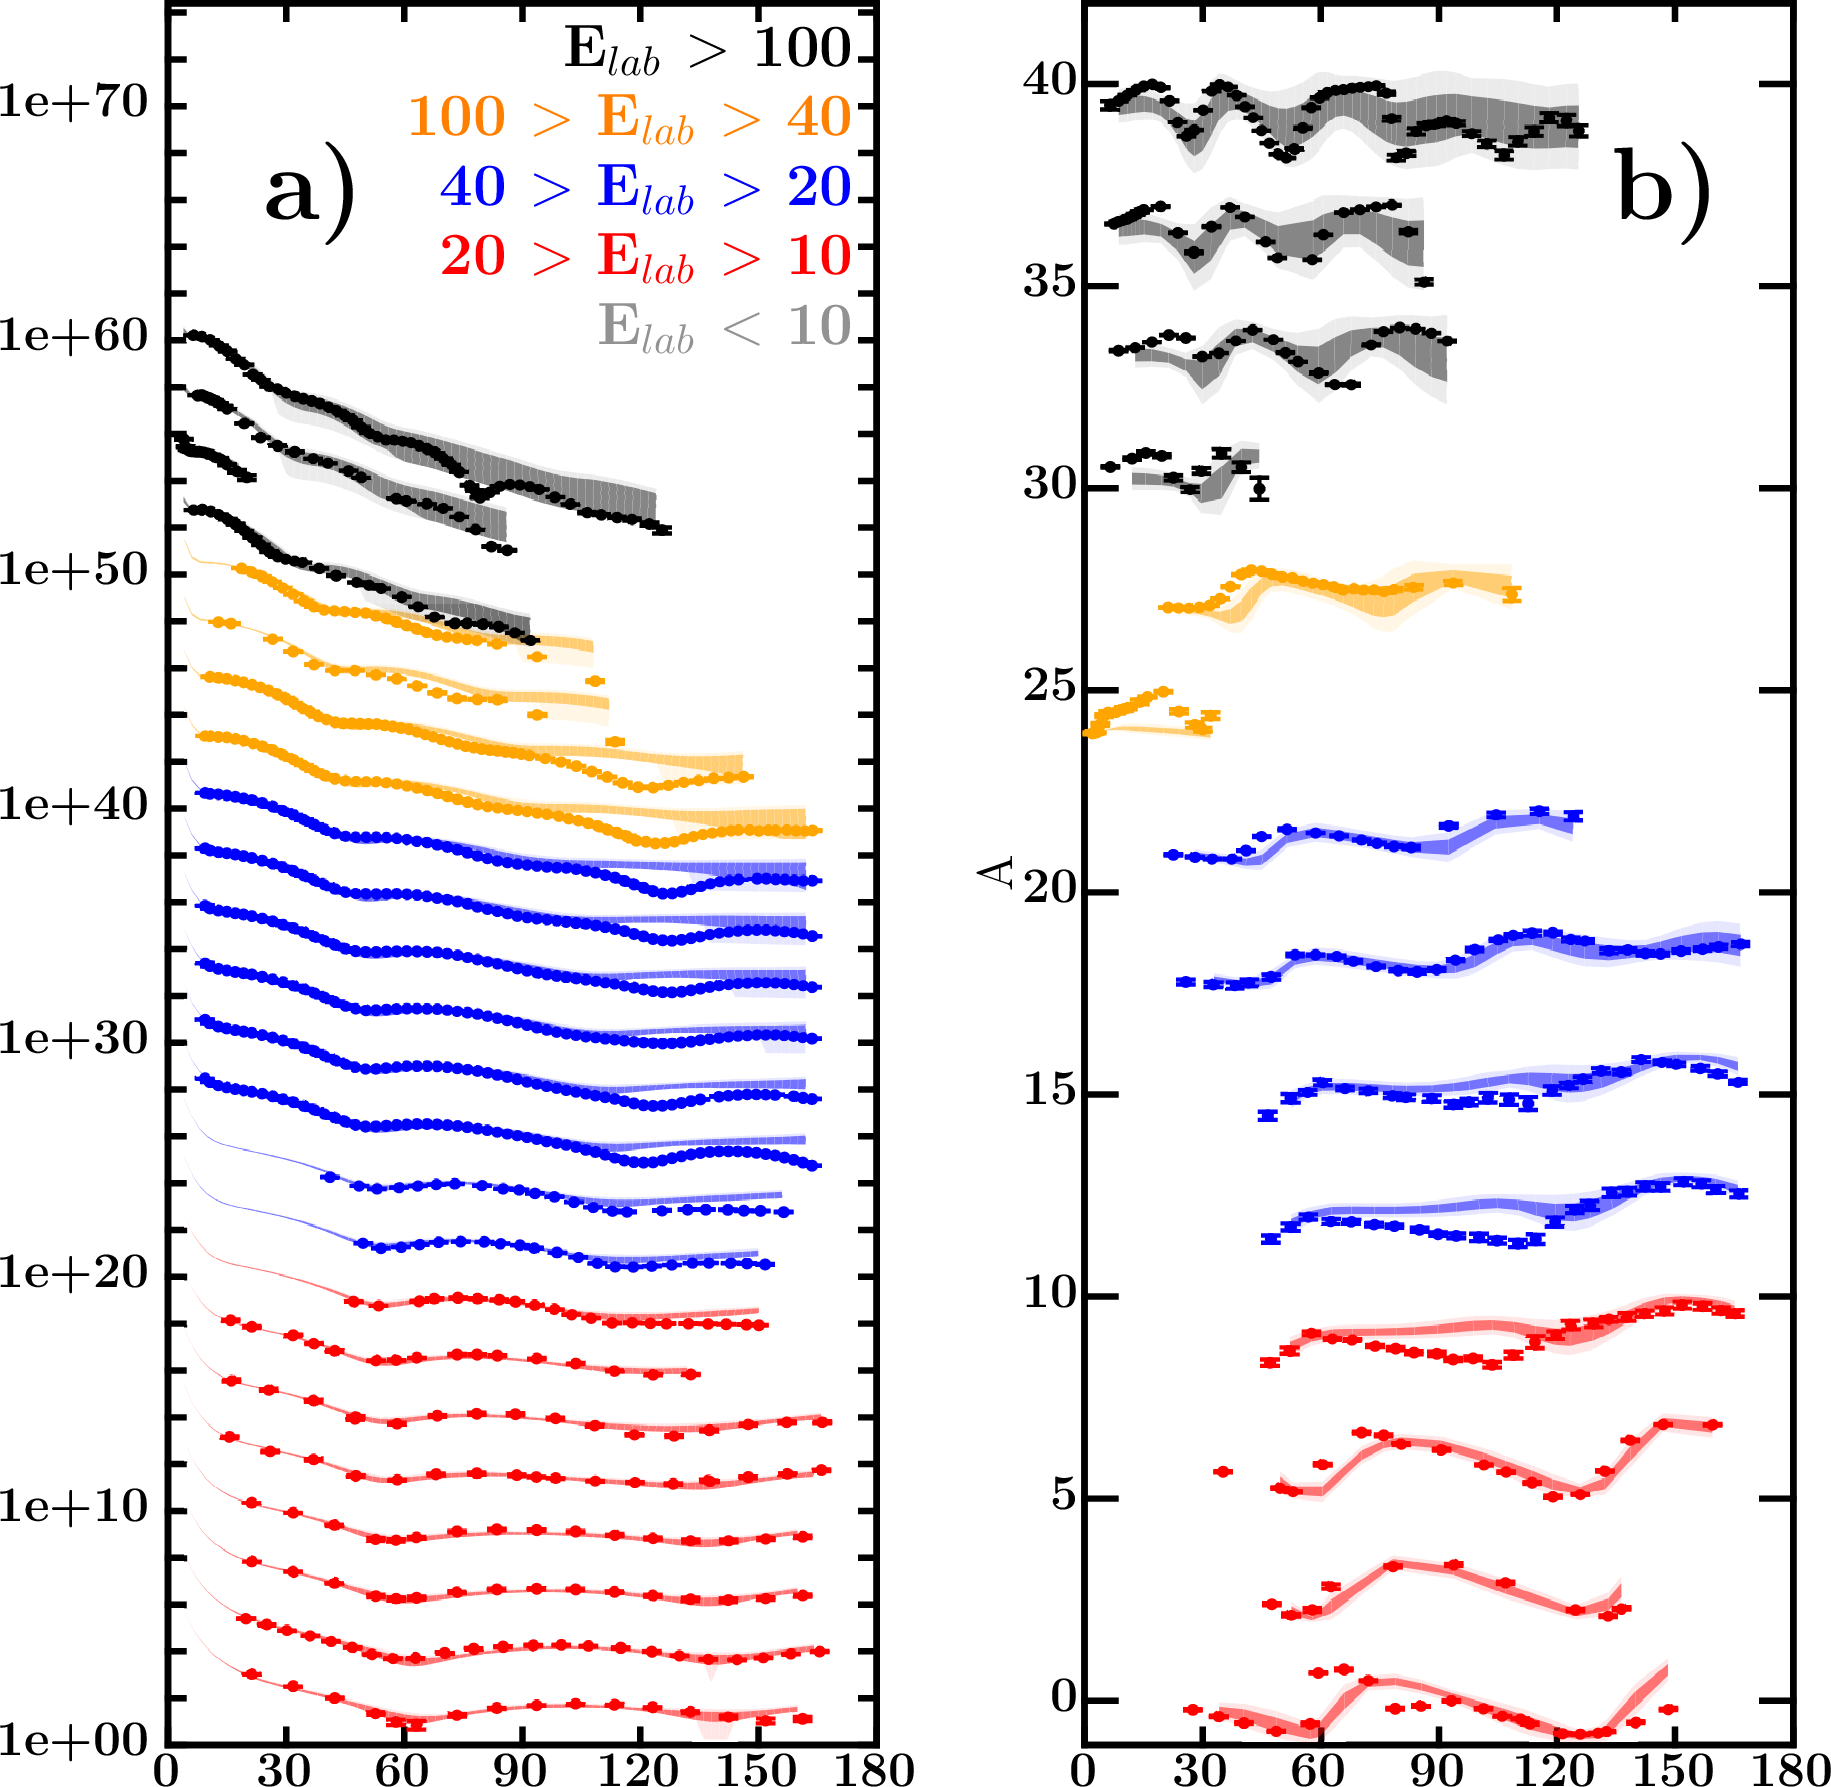
\includegraphics[width=\linewidth]{figures/o16_protonElastic.png}
        \label{DOM_o16_proton_elastic}
    \end{minipage}\hspace{6pt}
    \begin{minipage}{0.4\linewidth}
        \centering
        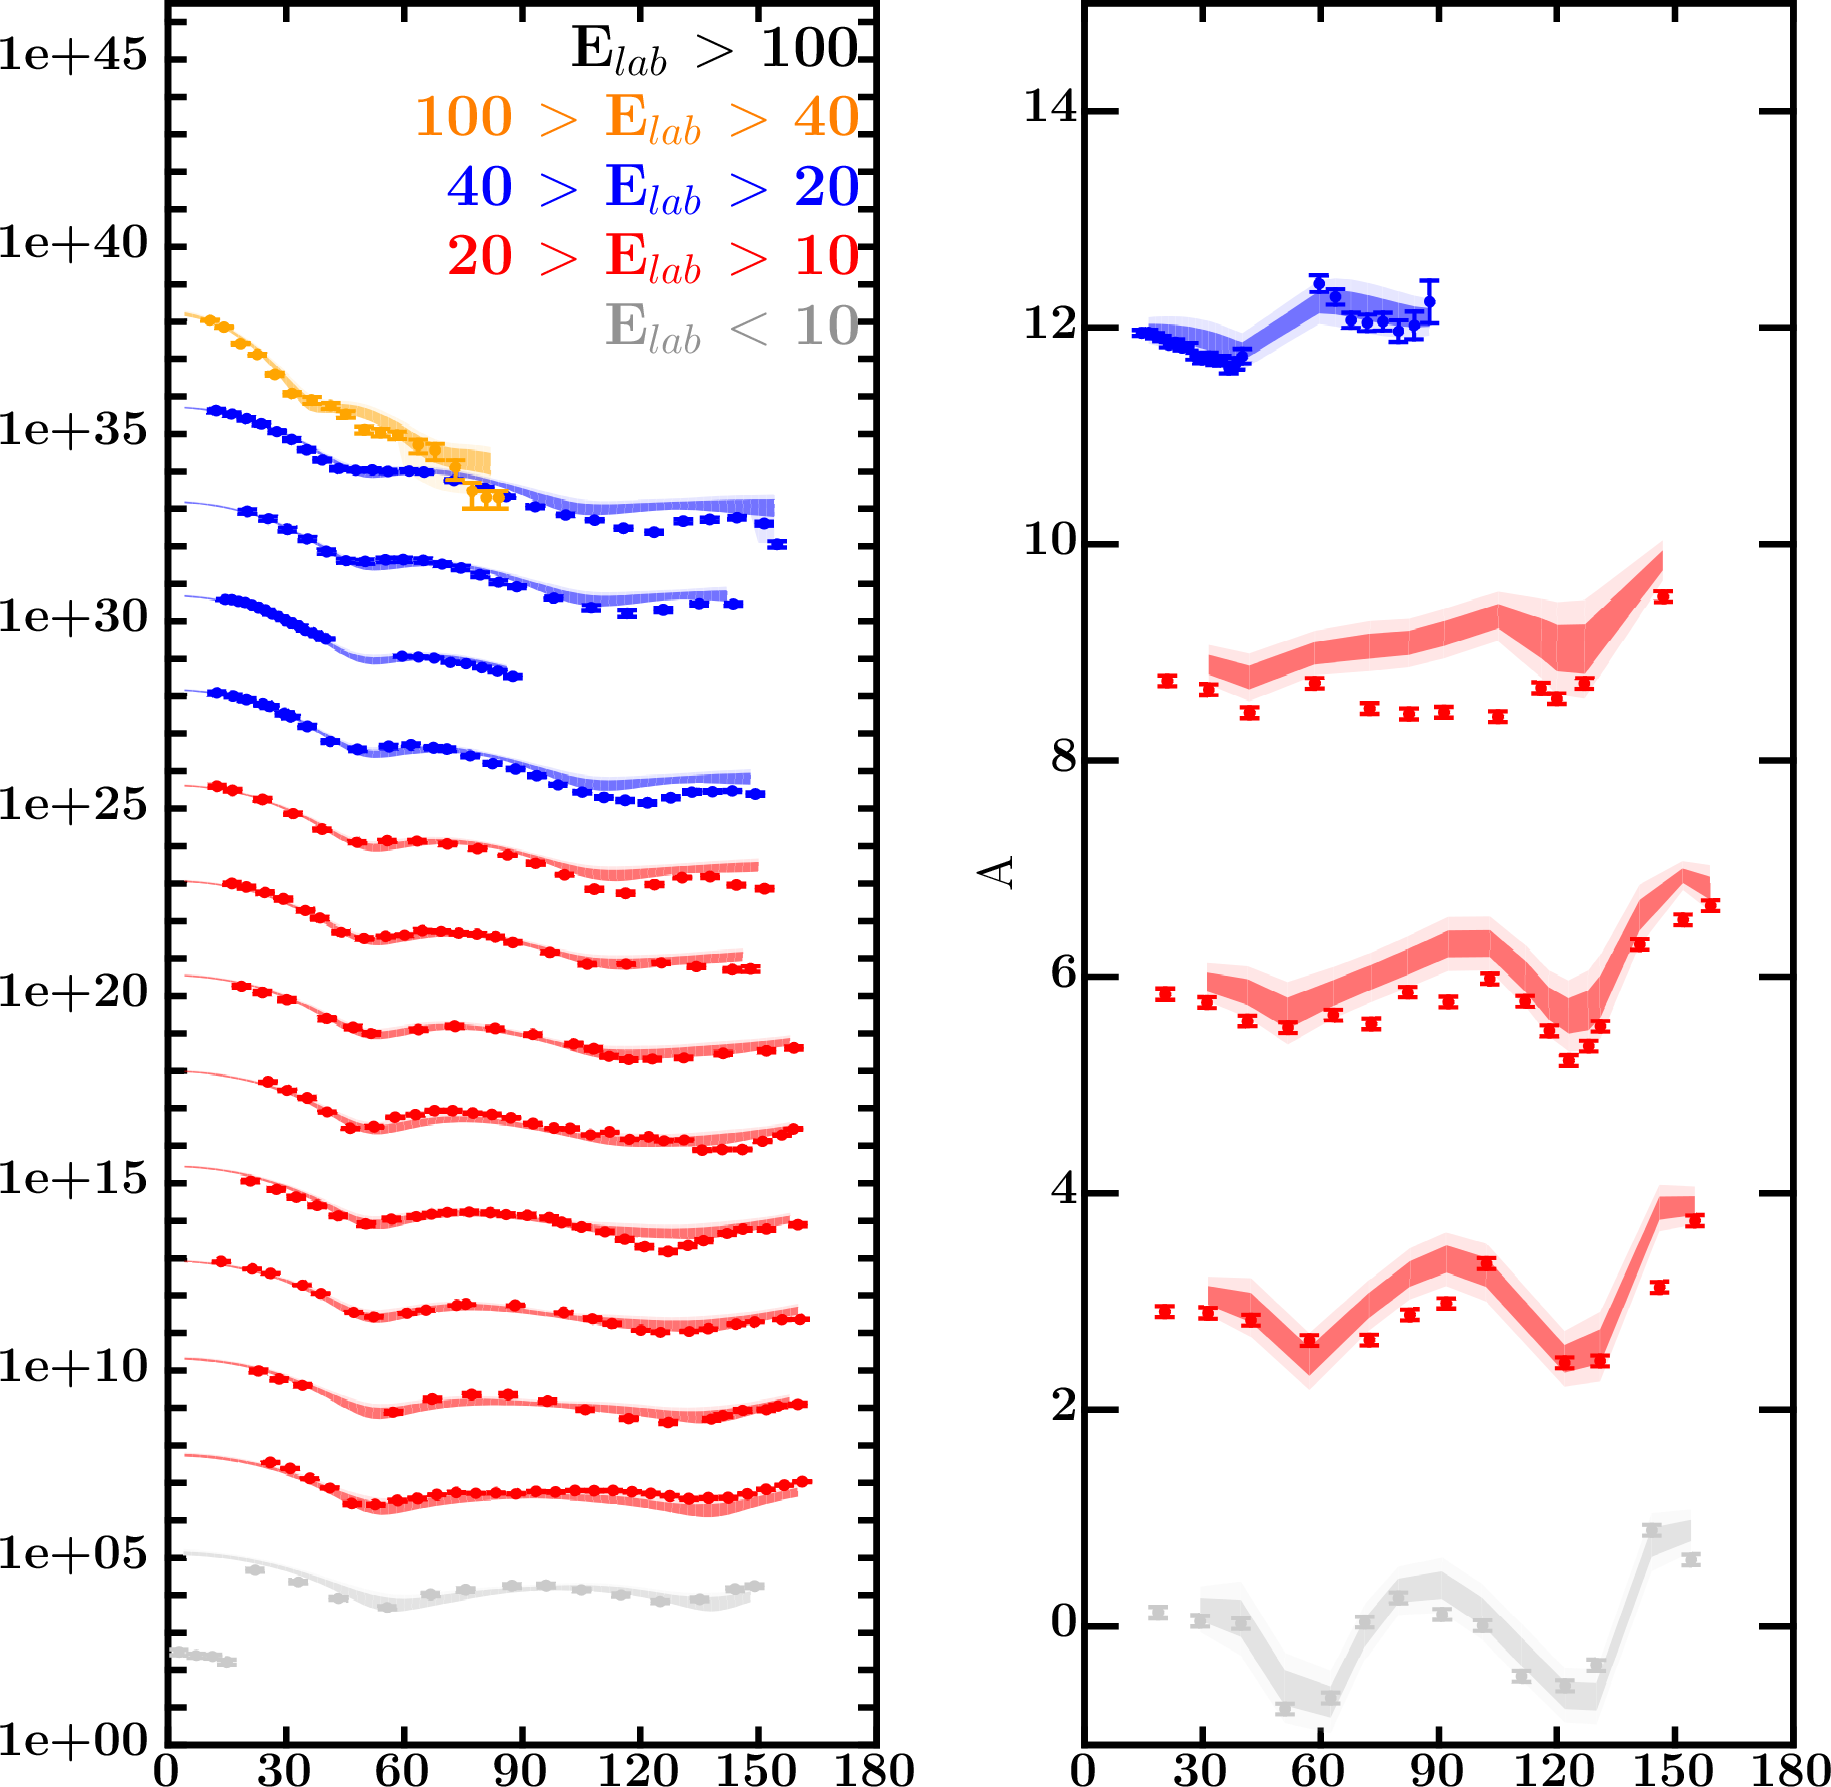
\includegraphics[width=\linewidth]{figures/o16_neutronElastic.png}
        \label{DOM_o16_neutron_elastic}
    \end{minipage}
    \centering
    \begin{minipage}{0.4\linewidth}
        \centering
        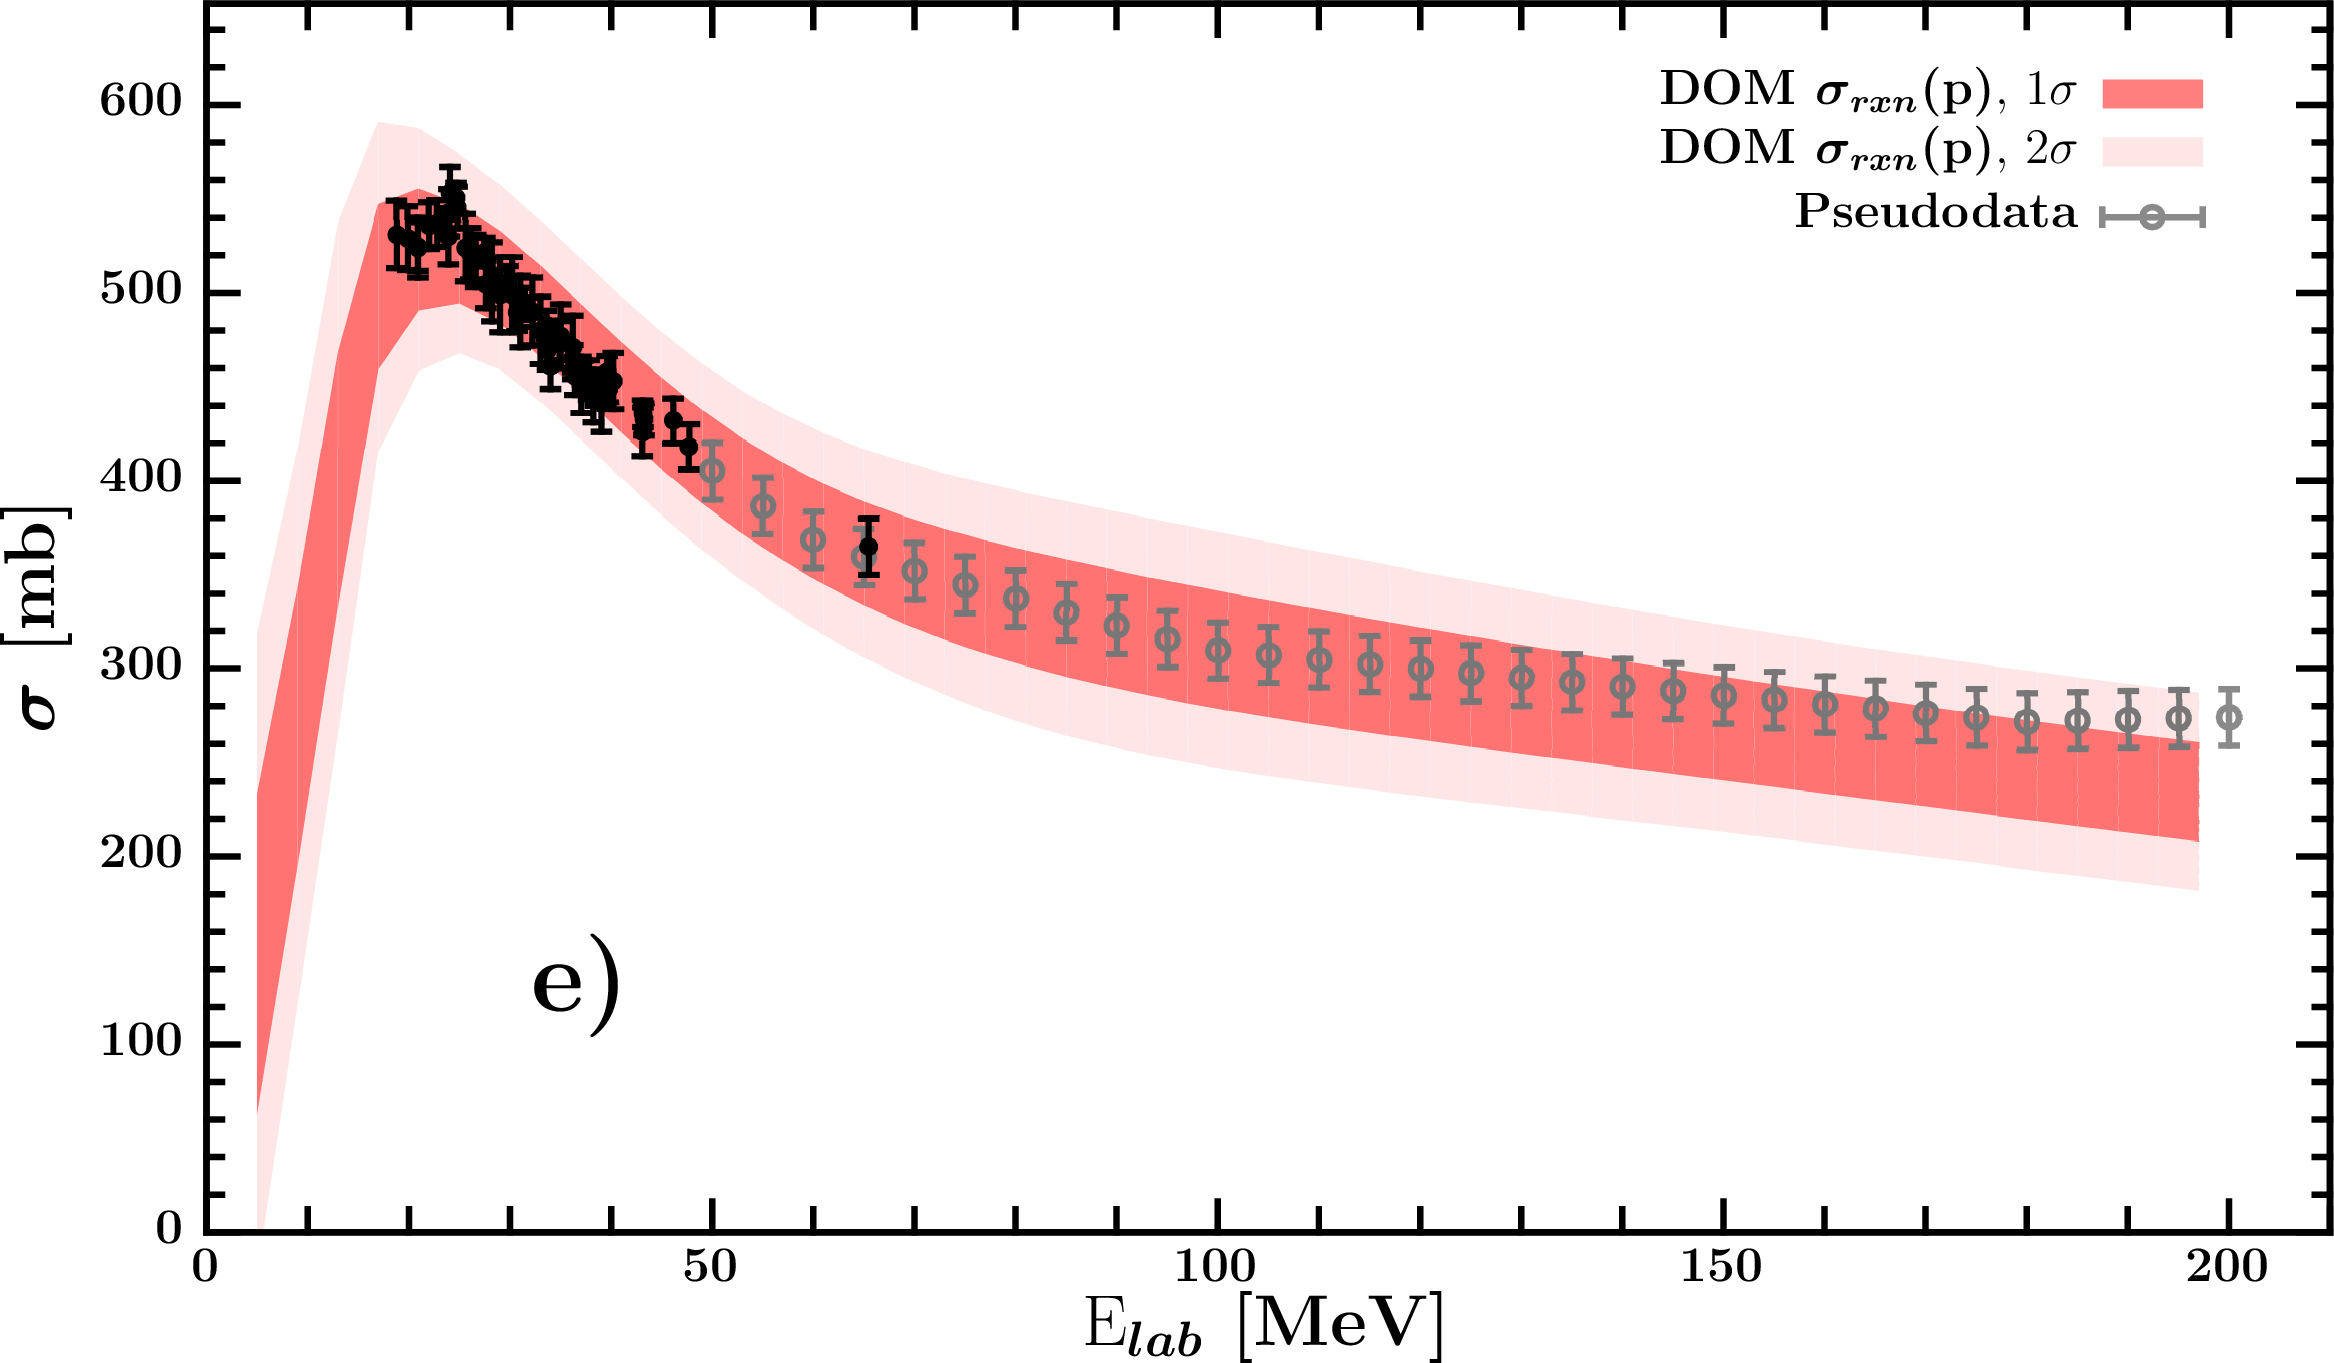
\includegraphics[width=\linewidth]{figures/o16_protonInelastic.png}
        \label{DOM_o16_proton_inelastic}
    \end{minipage}\hspace{6pt}
    \begin{minipage}{0.4\linewidth}
        \centering
        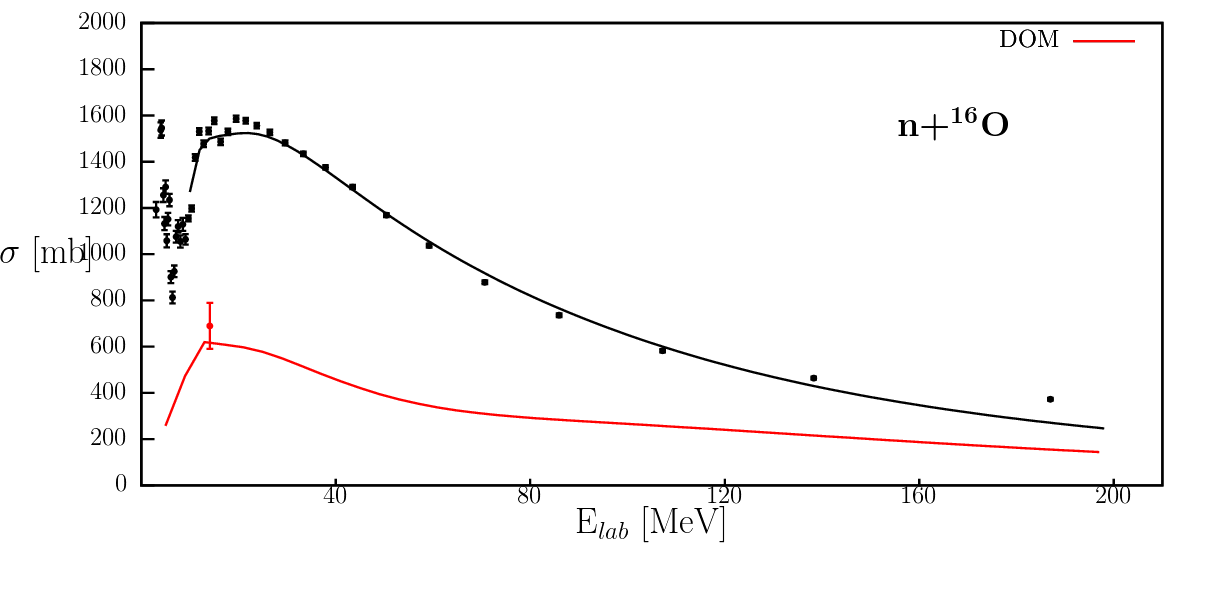
\includegraphics[width=\linewidth]{figures/o16_neutronInelastic.png}
        \label{DOM_o16_neutron_inelastic}
    \end{minipage}
    \caption{\oSix\ nucleon scattering data used in DOM fit}
    \label{DOM_o16_scattering}
    \centering
    \begin{minipage}{0.4\linewidth}
        \centering
        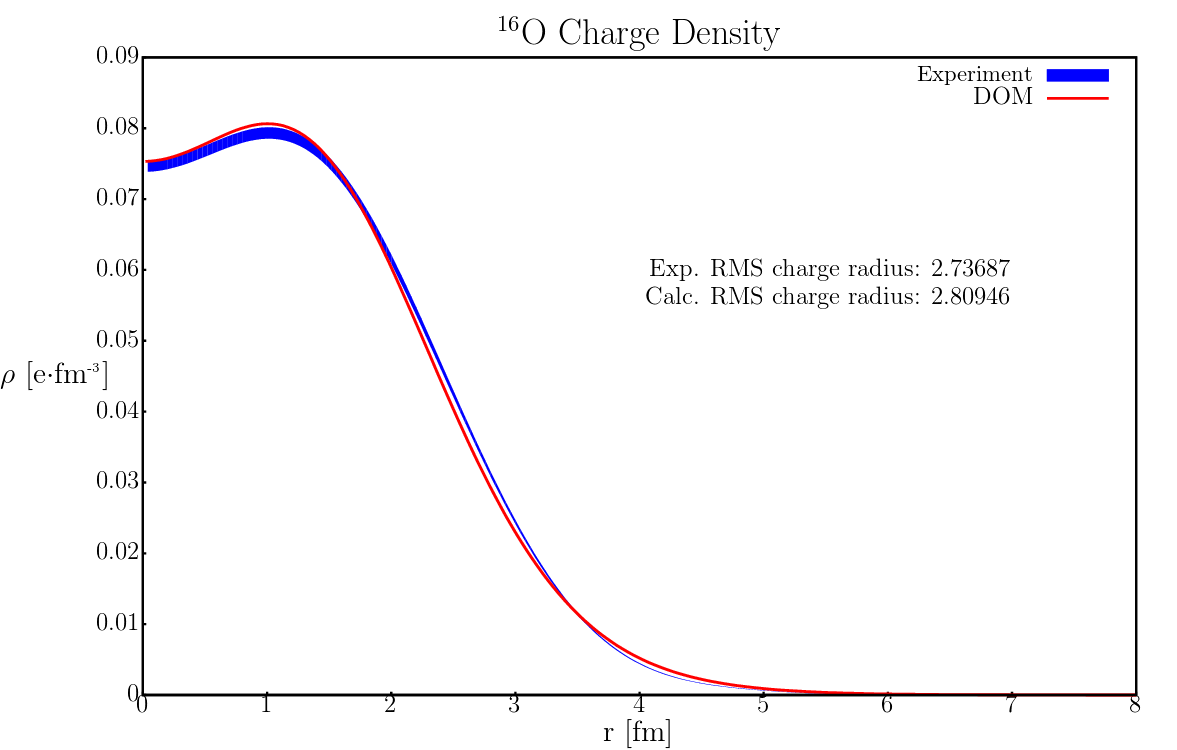
\includegraphics[width=\linewidth]{figures/o16_chargeDensity.png}
        \label{DOM_o16_chargeDensity}
    \end{minipage}
    \begin{minipage}{0.35\linewidth}
        \centering
        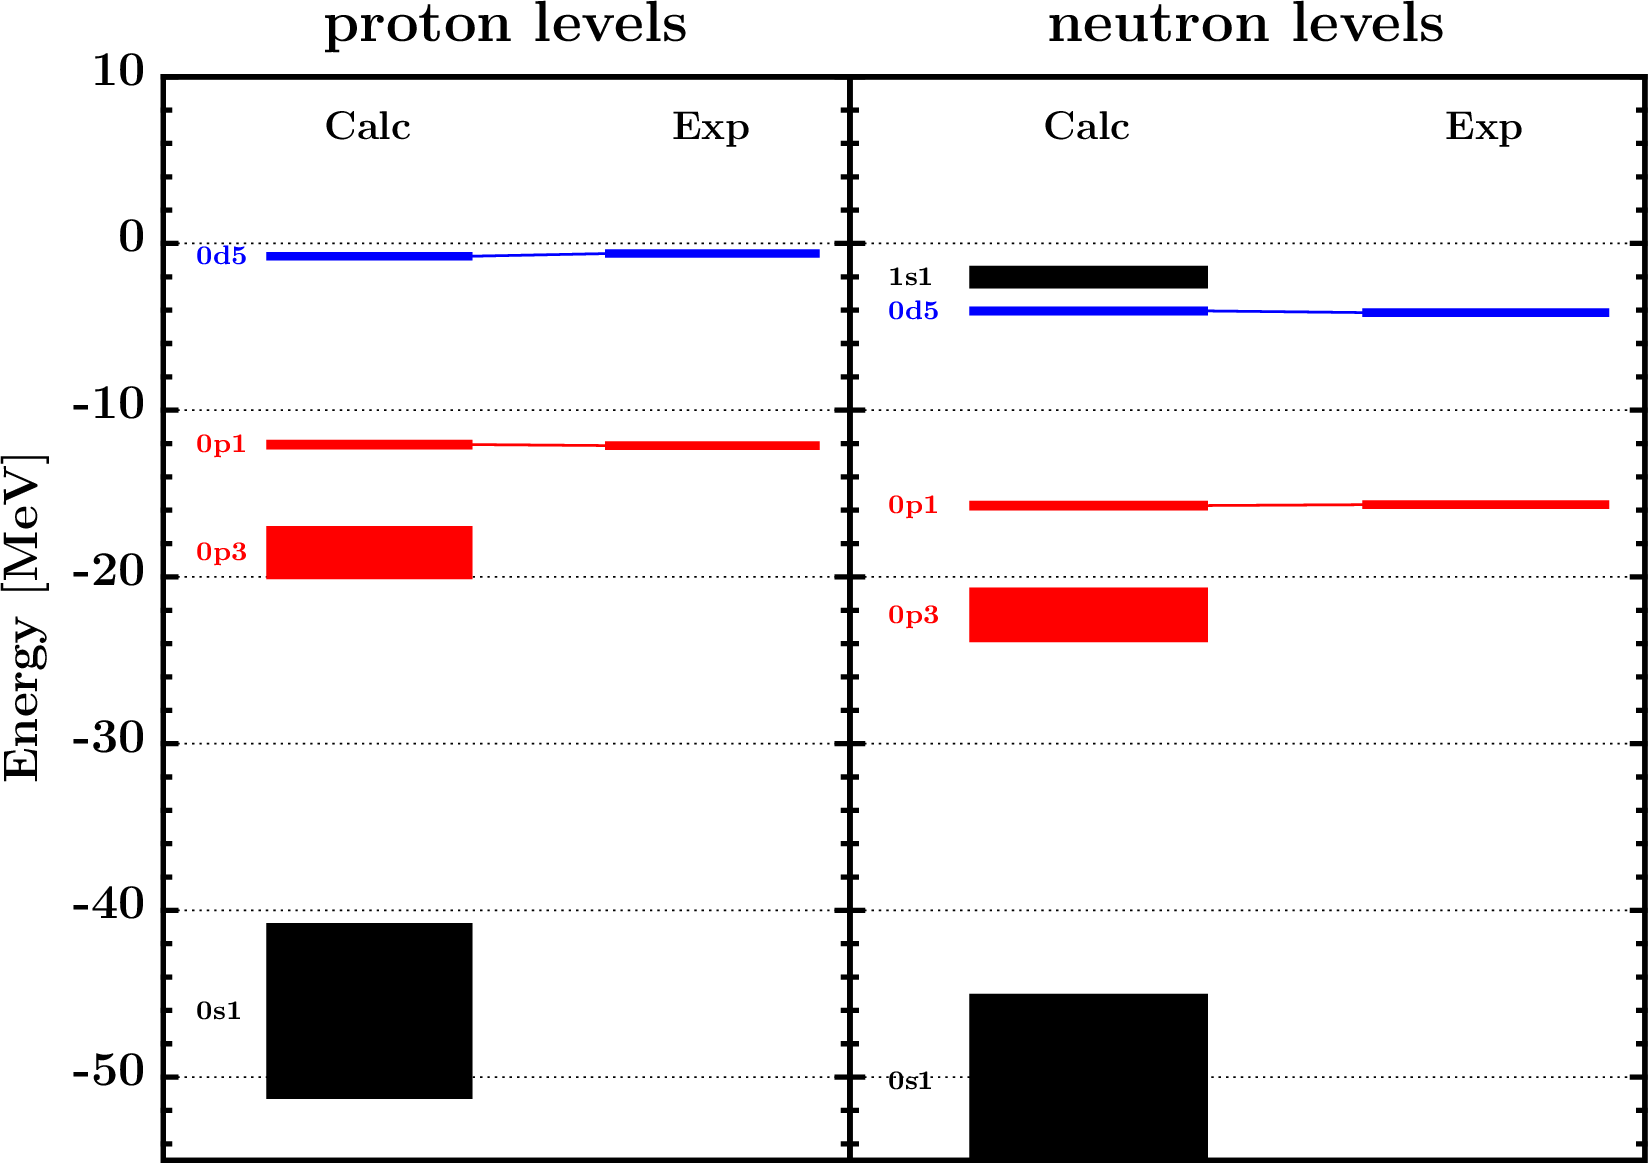
\includegraphics[width=\linewidth]{figures/o16_SPLevels.png}
        \label{DOM_o16_SPLevels}
    \end{minipage}
    \begin{minipage}{0.4\linewidth}
        \centering
        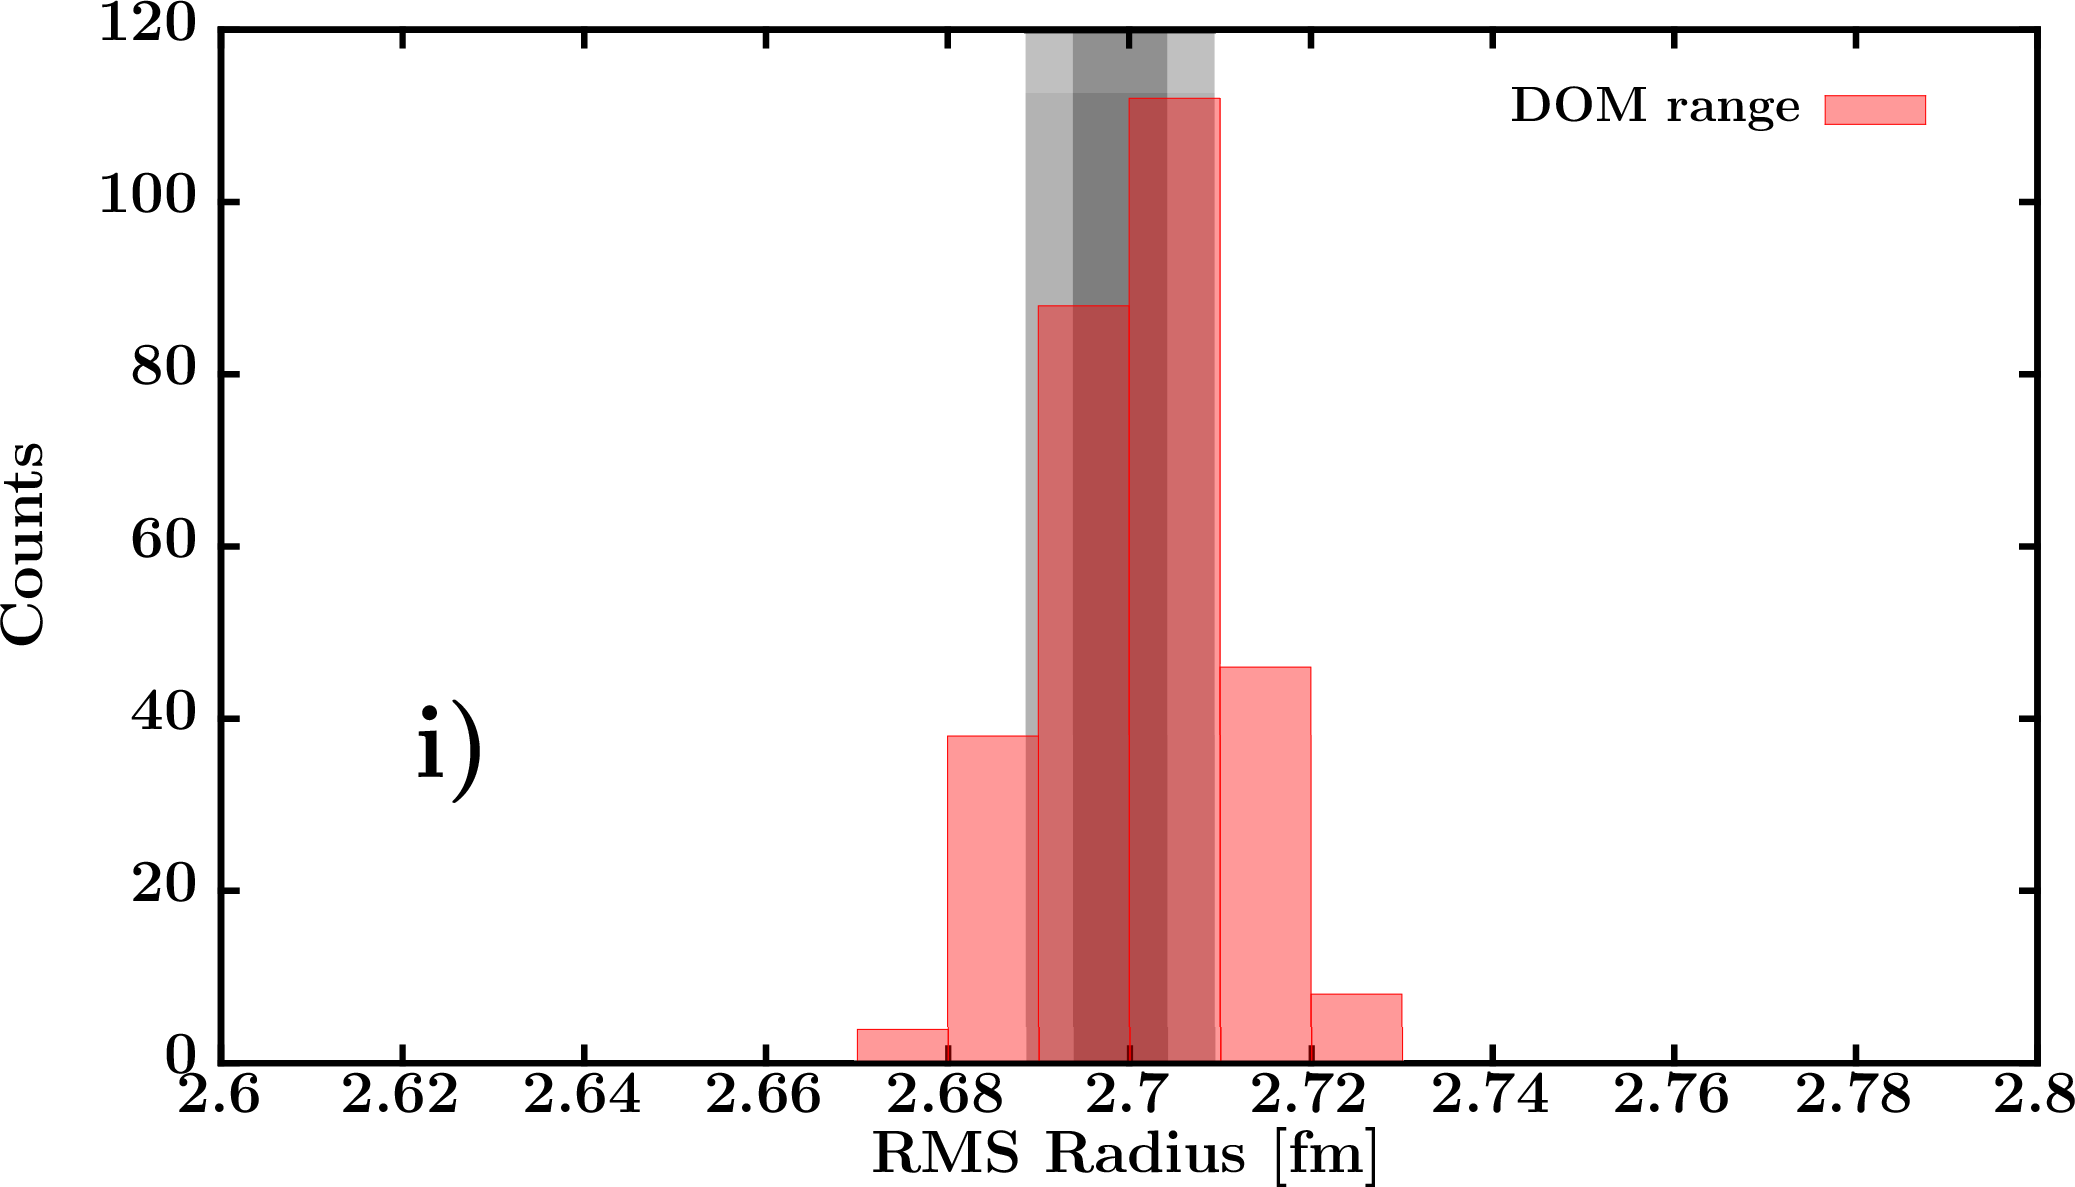
\includegraphics[width=\linewidth]{figures/o16_RMSRadius.png}
        \label{DOM_o16_RMSRadius}
    \end{minipage}
    \begin{minipage}{0.4\linewidth}
        \centering
        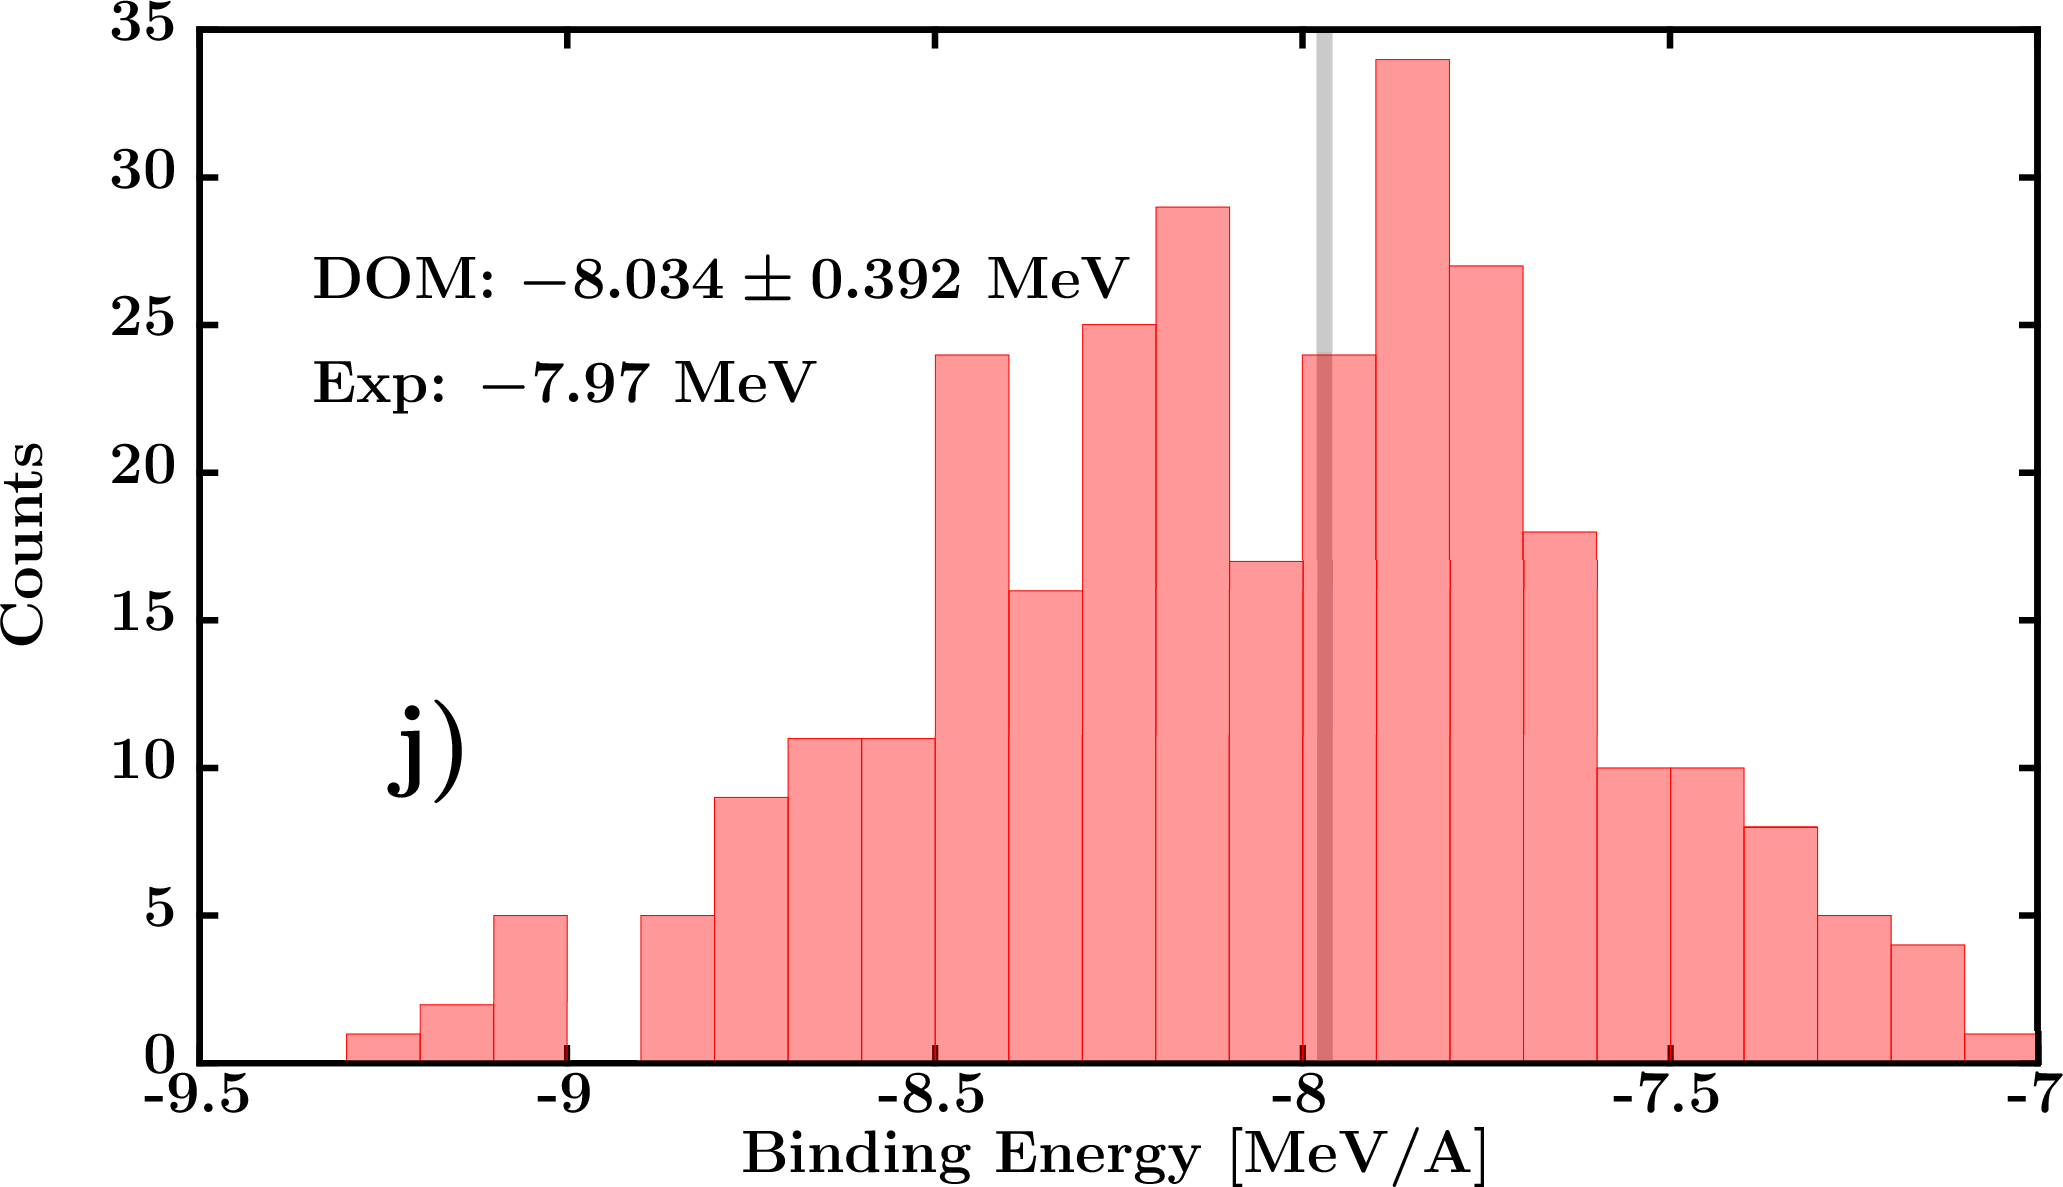
\includegraphics[width=\linewidth]{figures/o16_BE.png}
        \label{DOM_o16_BE}
    \end{minipage}
    \caption{\oSix\ bound-state data used in DOM fit}
    \label{DOM_o16_structural}
\end{figure*}

\begin{figure*}[!htb]
    \centering
    \begin{minipage}{0.4\linewidth}
        \centering
        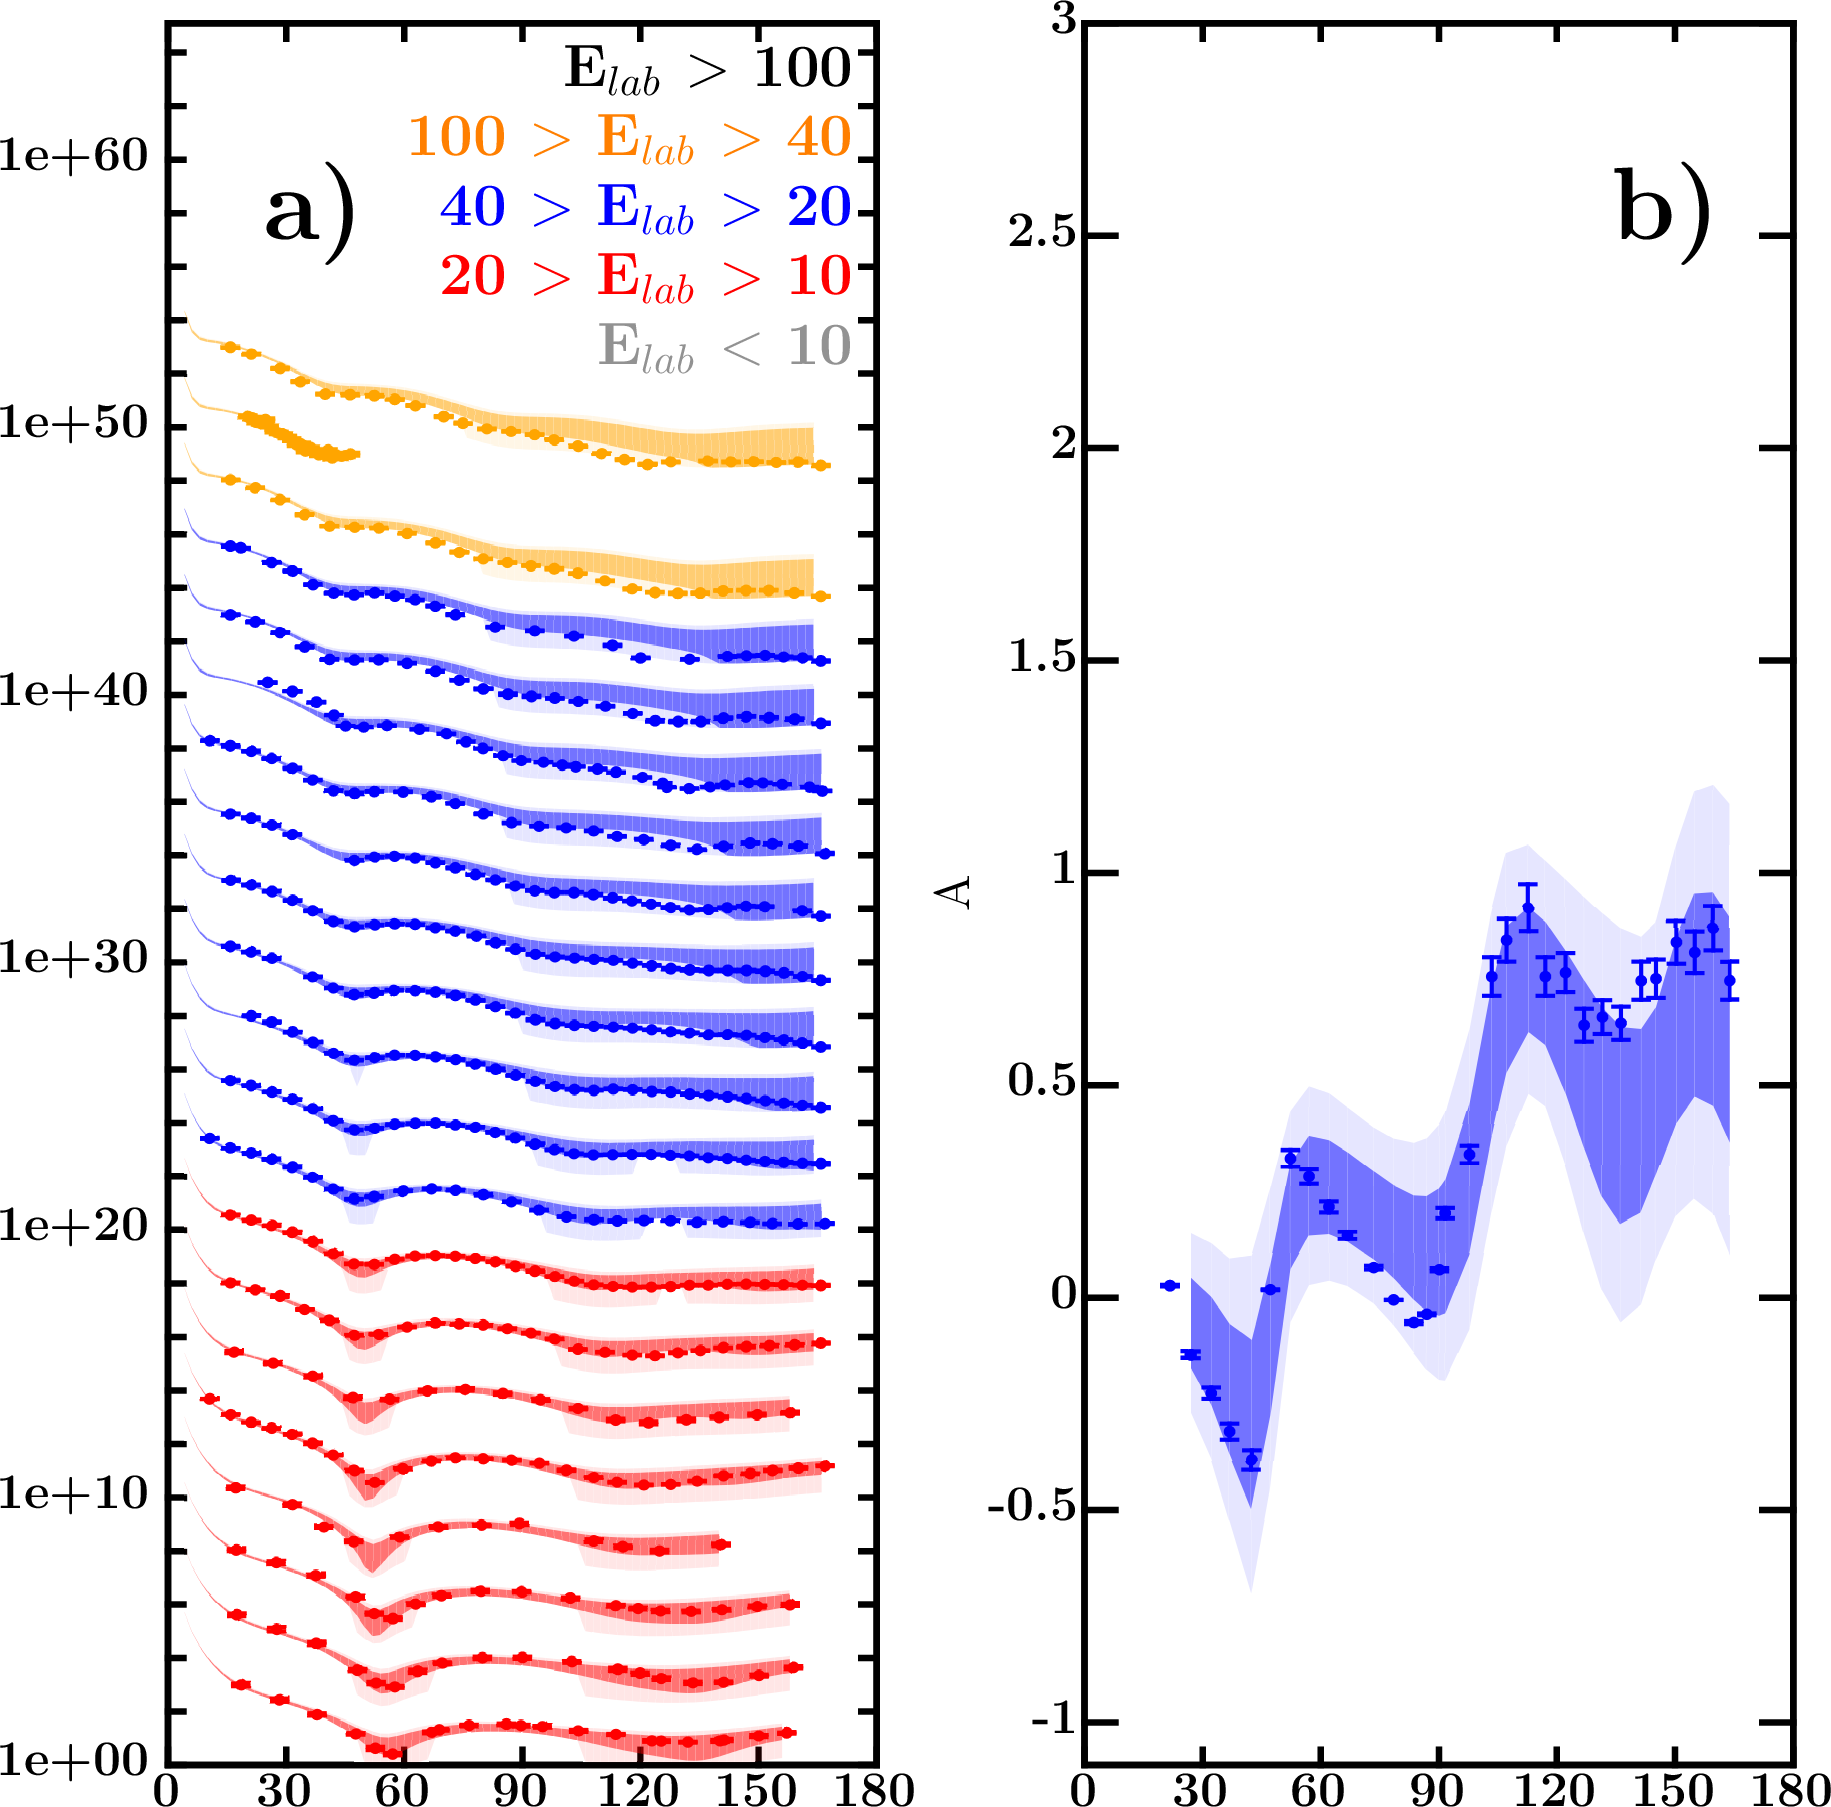
\includegraphics[width=\linewidth]{figures/o18_protonElastic.png}
        \label{DOM_o18_proton_elastic}
    \end{minipage}
    \begin{minipage}{0.4\linewidth}
        \centering
        \begin{minipage}[c]{0.5\linewidth}
            \centering
            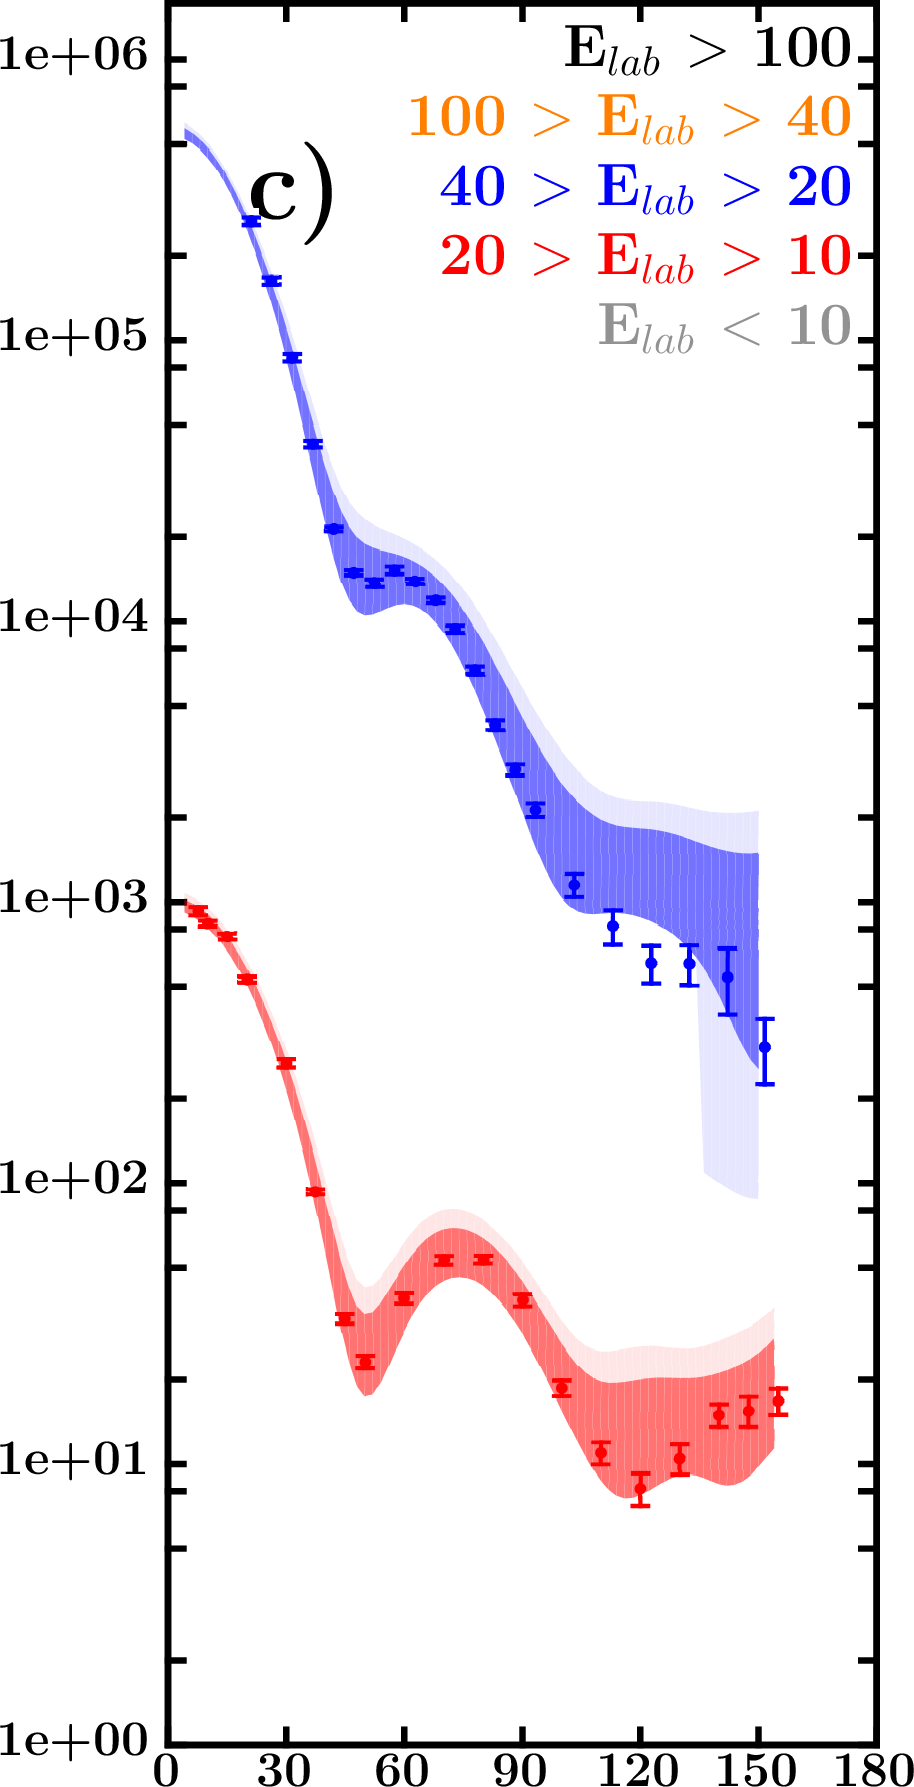
\includegraphics[width=\linewidth]{figures/o18_neutronElastic.png}
        \end{minipage}
        \begin{minipage}[c]{0.4\linewidth}
            \centering
            No \oEight\\
            proton \rxn\ data\\
            were available
        \end{minipage}
        \label{DOM_o18_neutron_elastic}
    \end{minipage}
    \centering
    \begin{minipage}{0.4\linewidth}
        \centering
        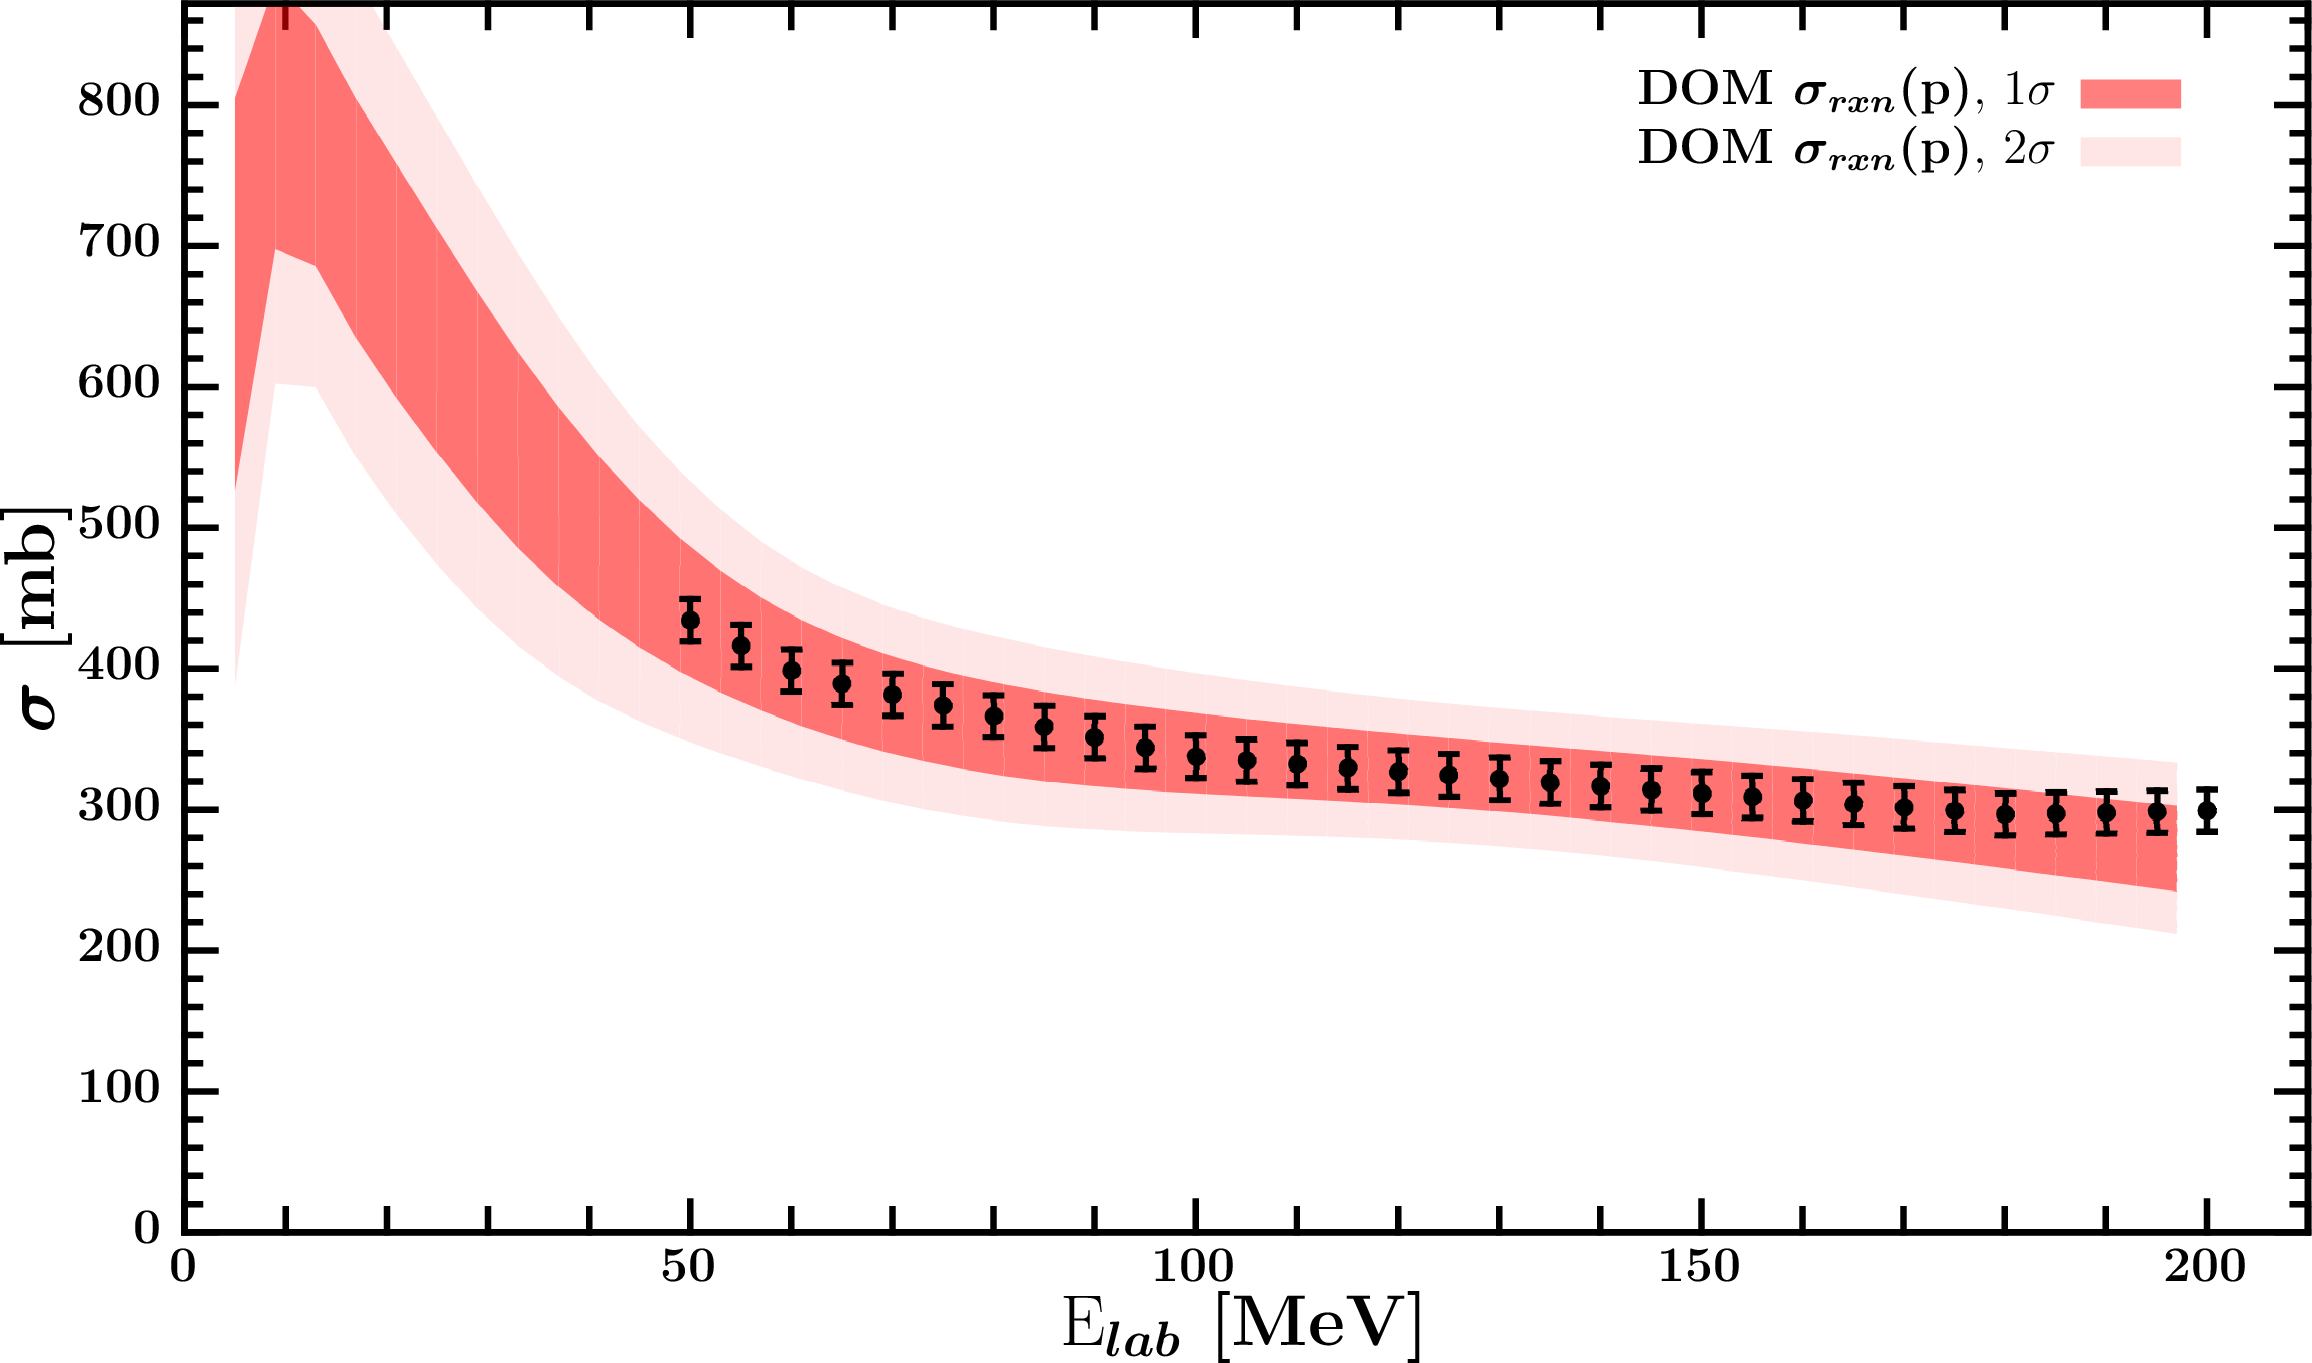
\includegraphics[width=\linewidth]{figures/o18_protonInelastic.png}
        \label{DOM_o18_proton_inelastic}
    \end{minipage}\hspace{6pt}
    \begin{minipage}{0.4\linewidth}
        \centering
        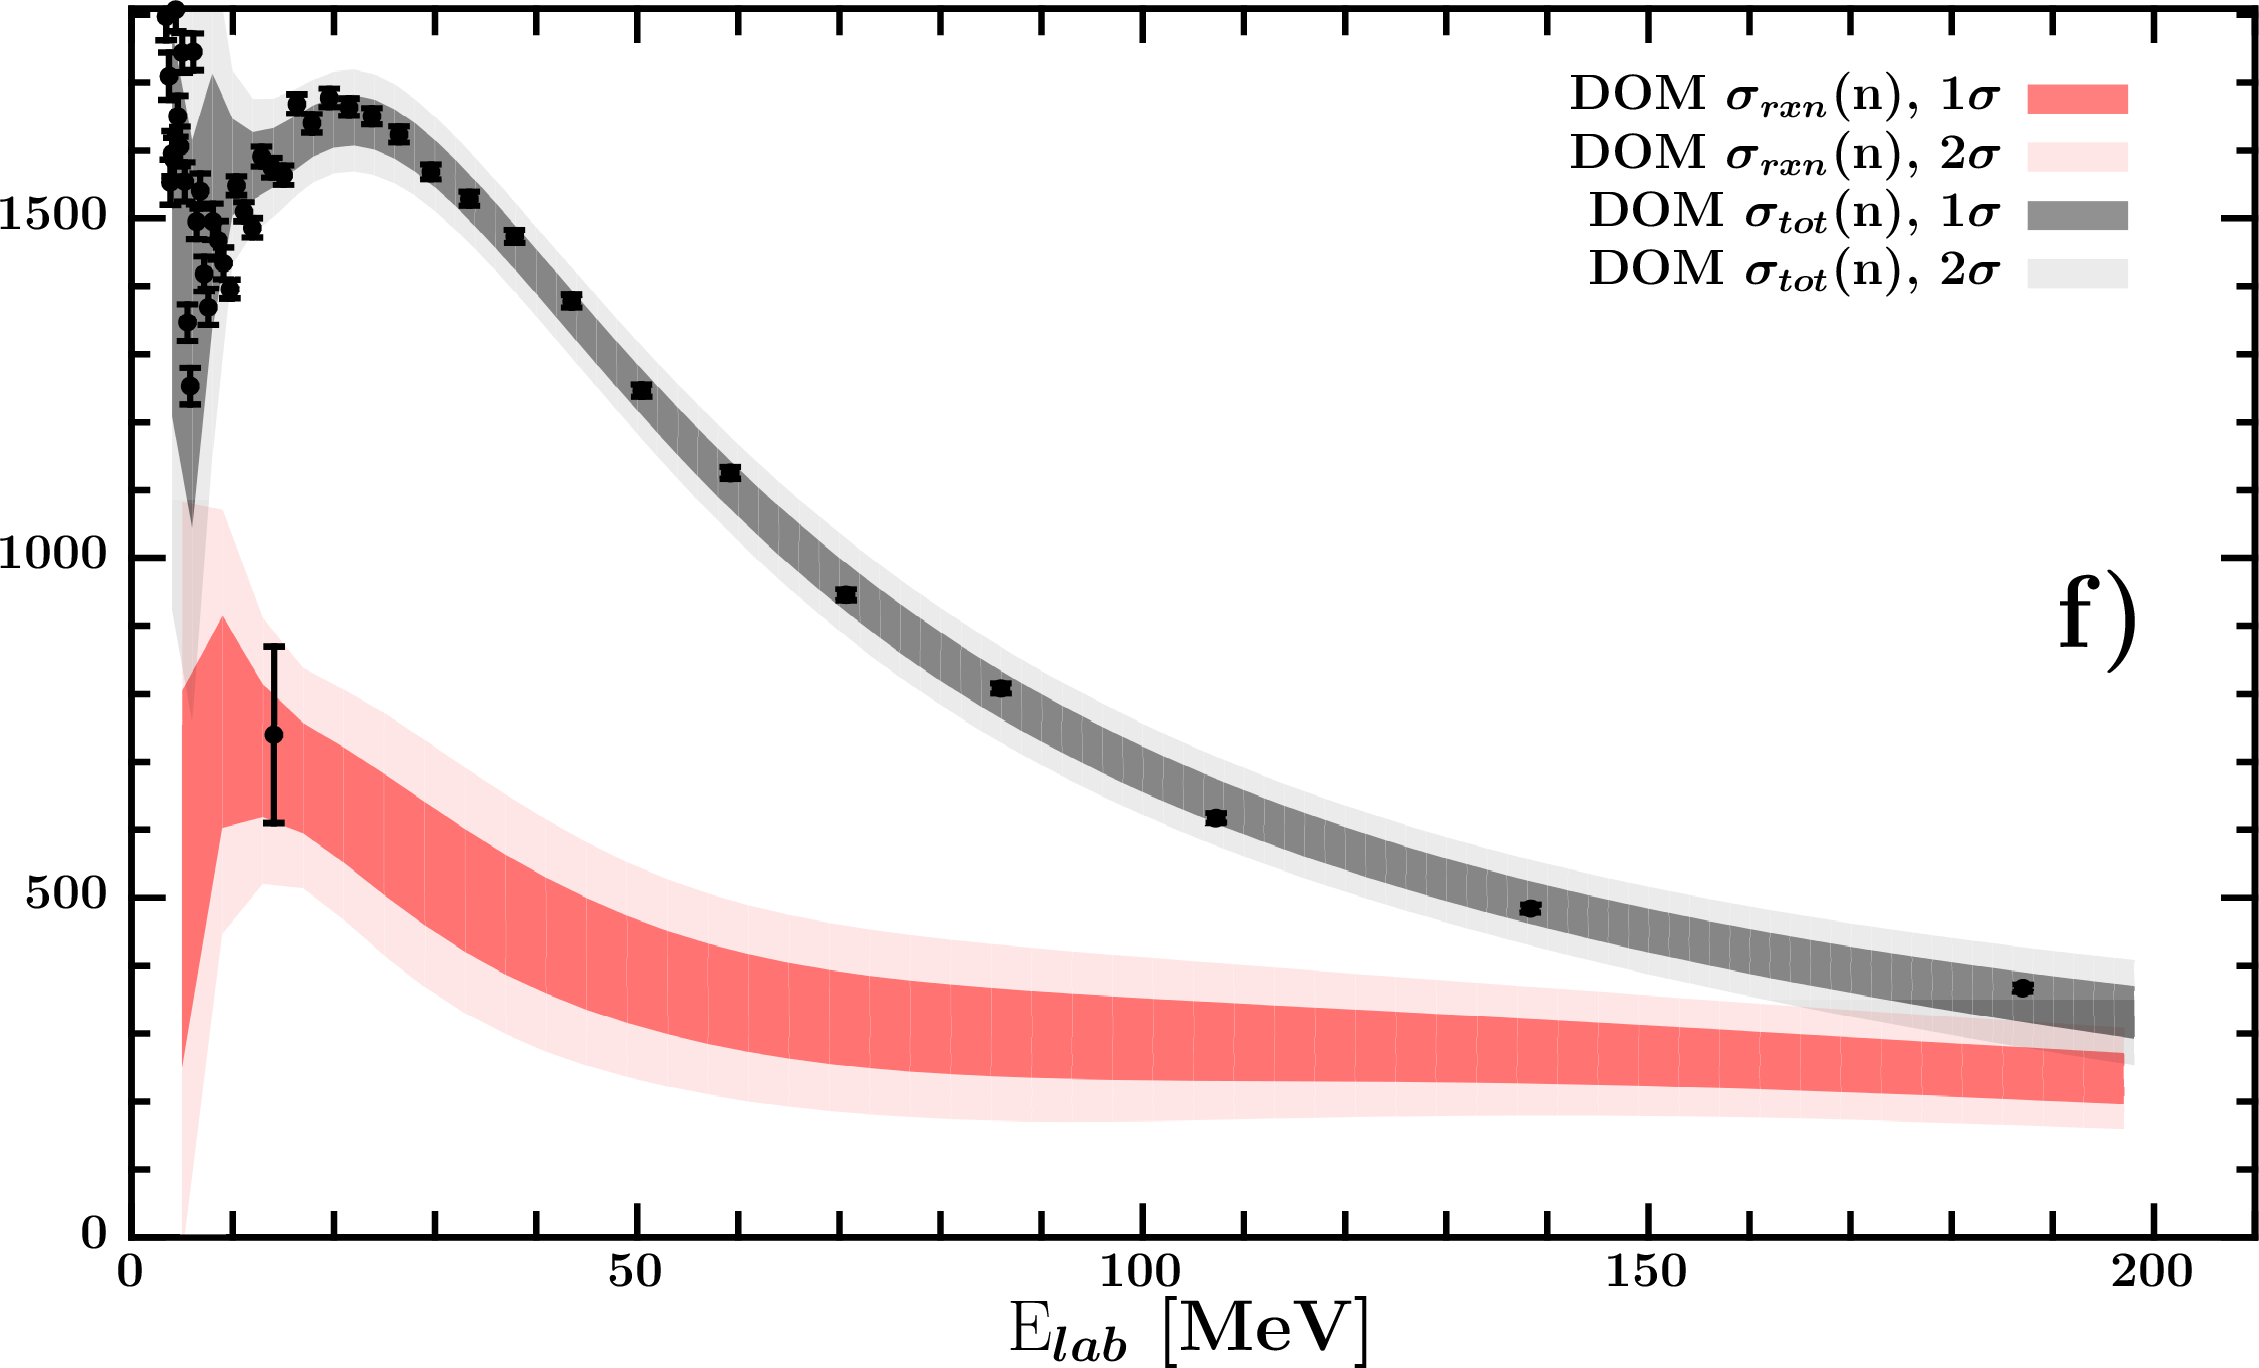
\includegraphics[width=\linewidth]{figures/o18_neutronInelastic.png}
        \label{DOM_o18_neutron_inelastic}
    \end{minipage}
    \caption{\oEight\ nucleon scattering data used in DOM fit}
    \label{DOM_o18_scattering}
    \centering
    \begin{minipage}{0.4\linewidth}
        \centering
        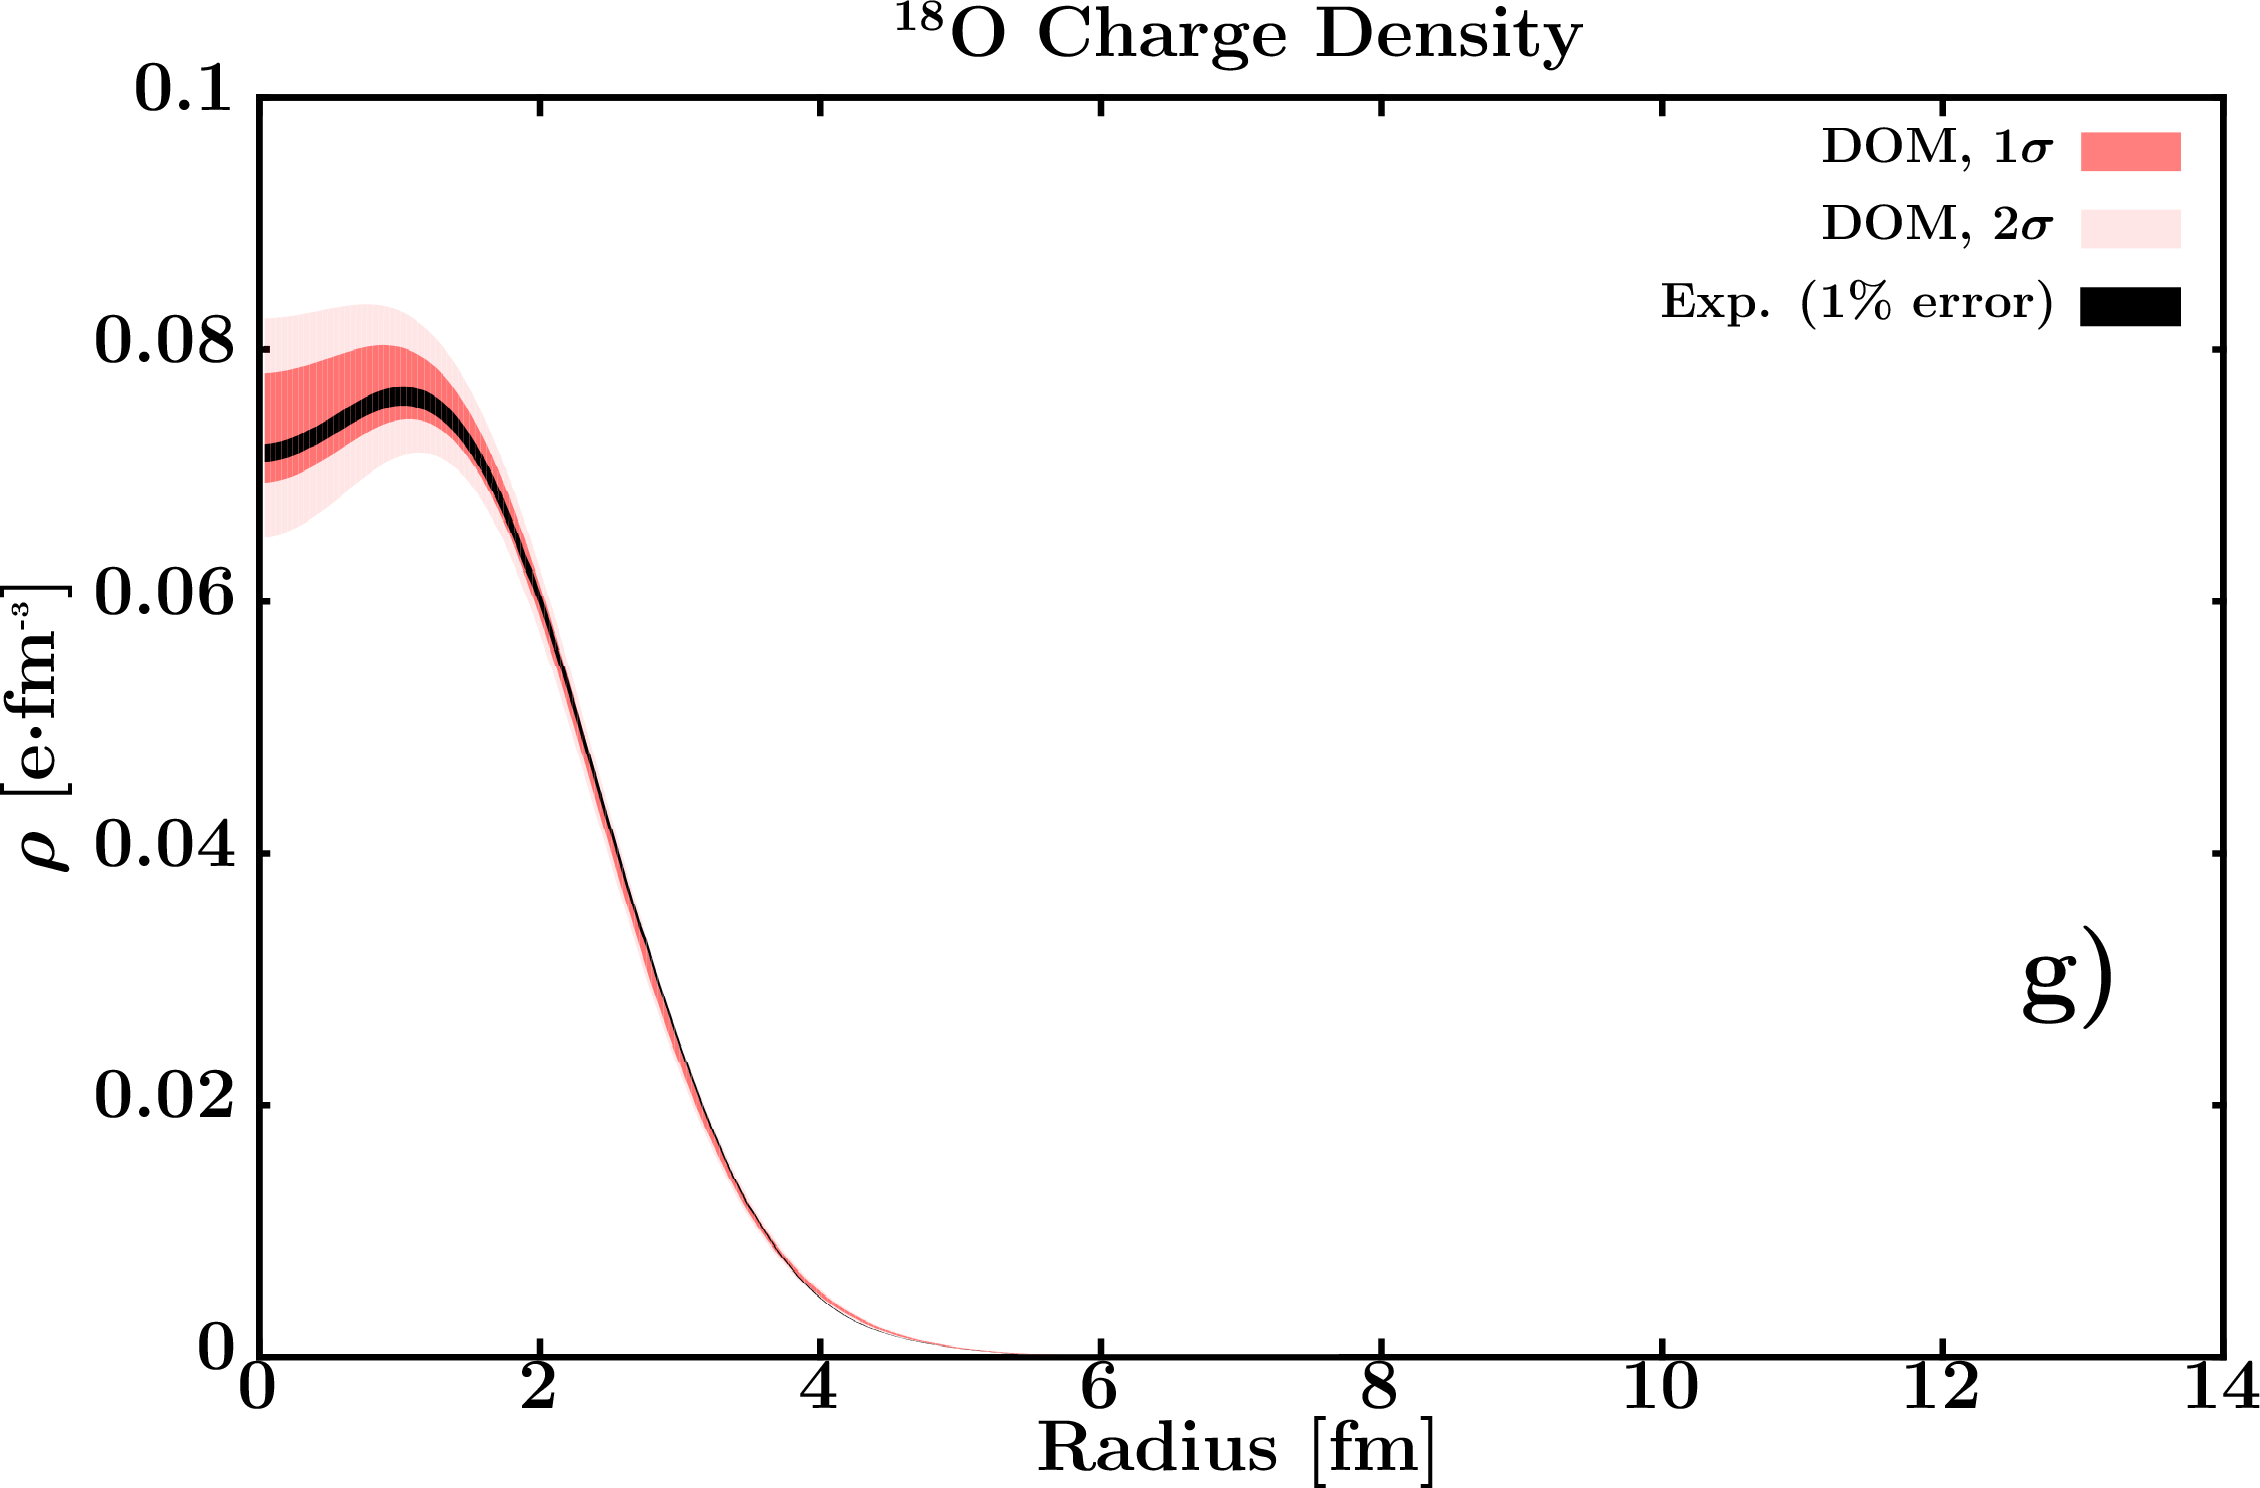
\includegraphics[width=\linewidth]{figures/o18_chargeDensity.png}
        \label{DOM_o18_chargeDensity}
    \end{minipage}
    \begin{minipage}{0.35\linewidth}
        \centering
        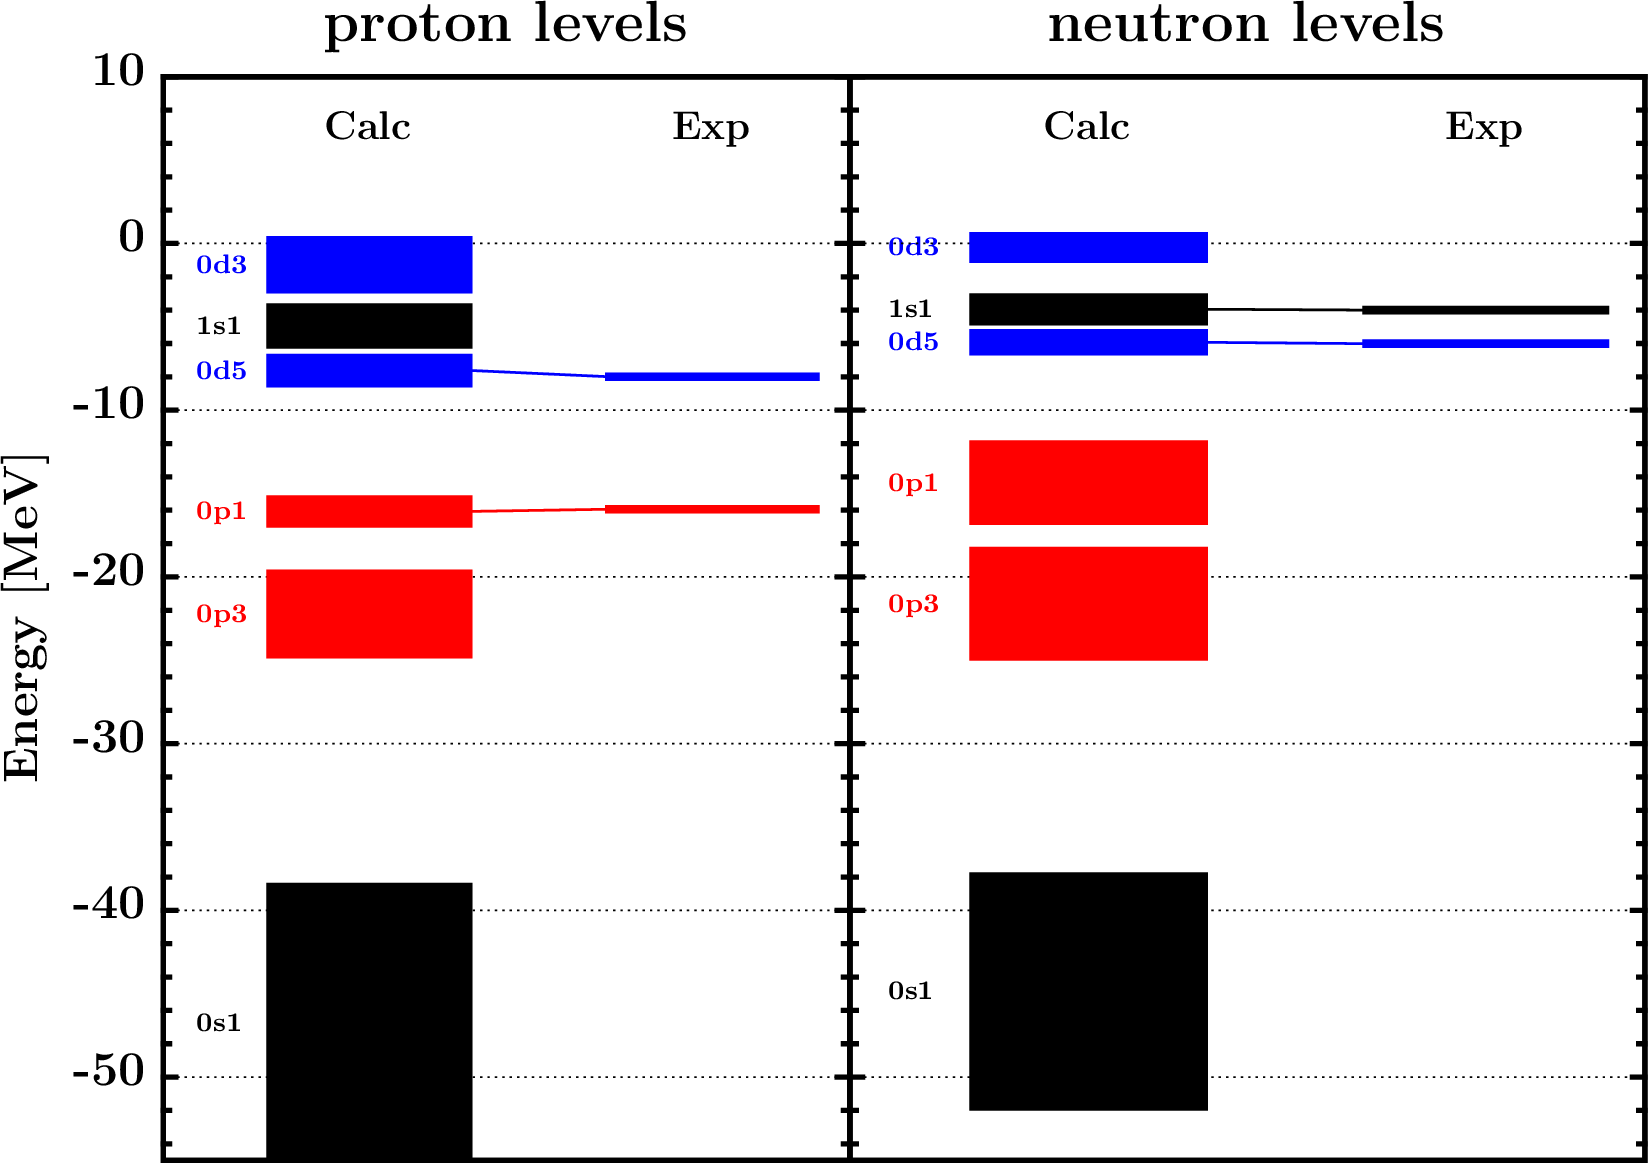
\includegraphics[width=\linewidth]{figures/o18_SPLevels.png}
        \label{DOM_o18_SPLevels}
    \end{minipage}
    \begin{minipage}{0.4\linewidth}
        \centering
        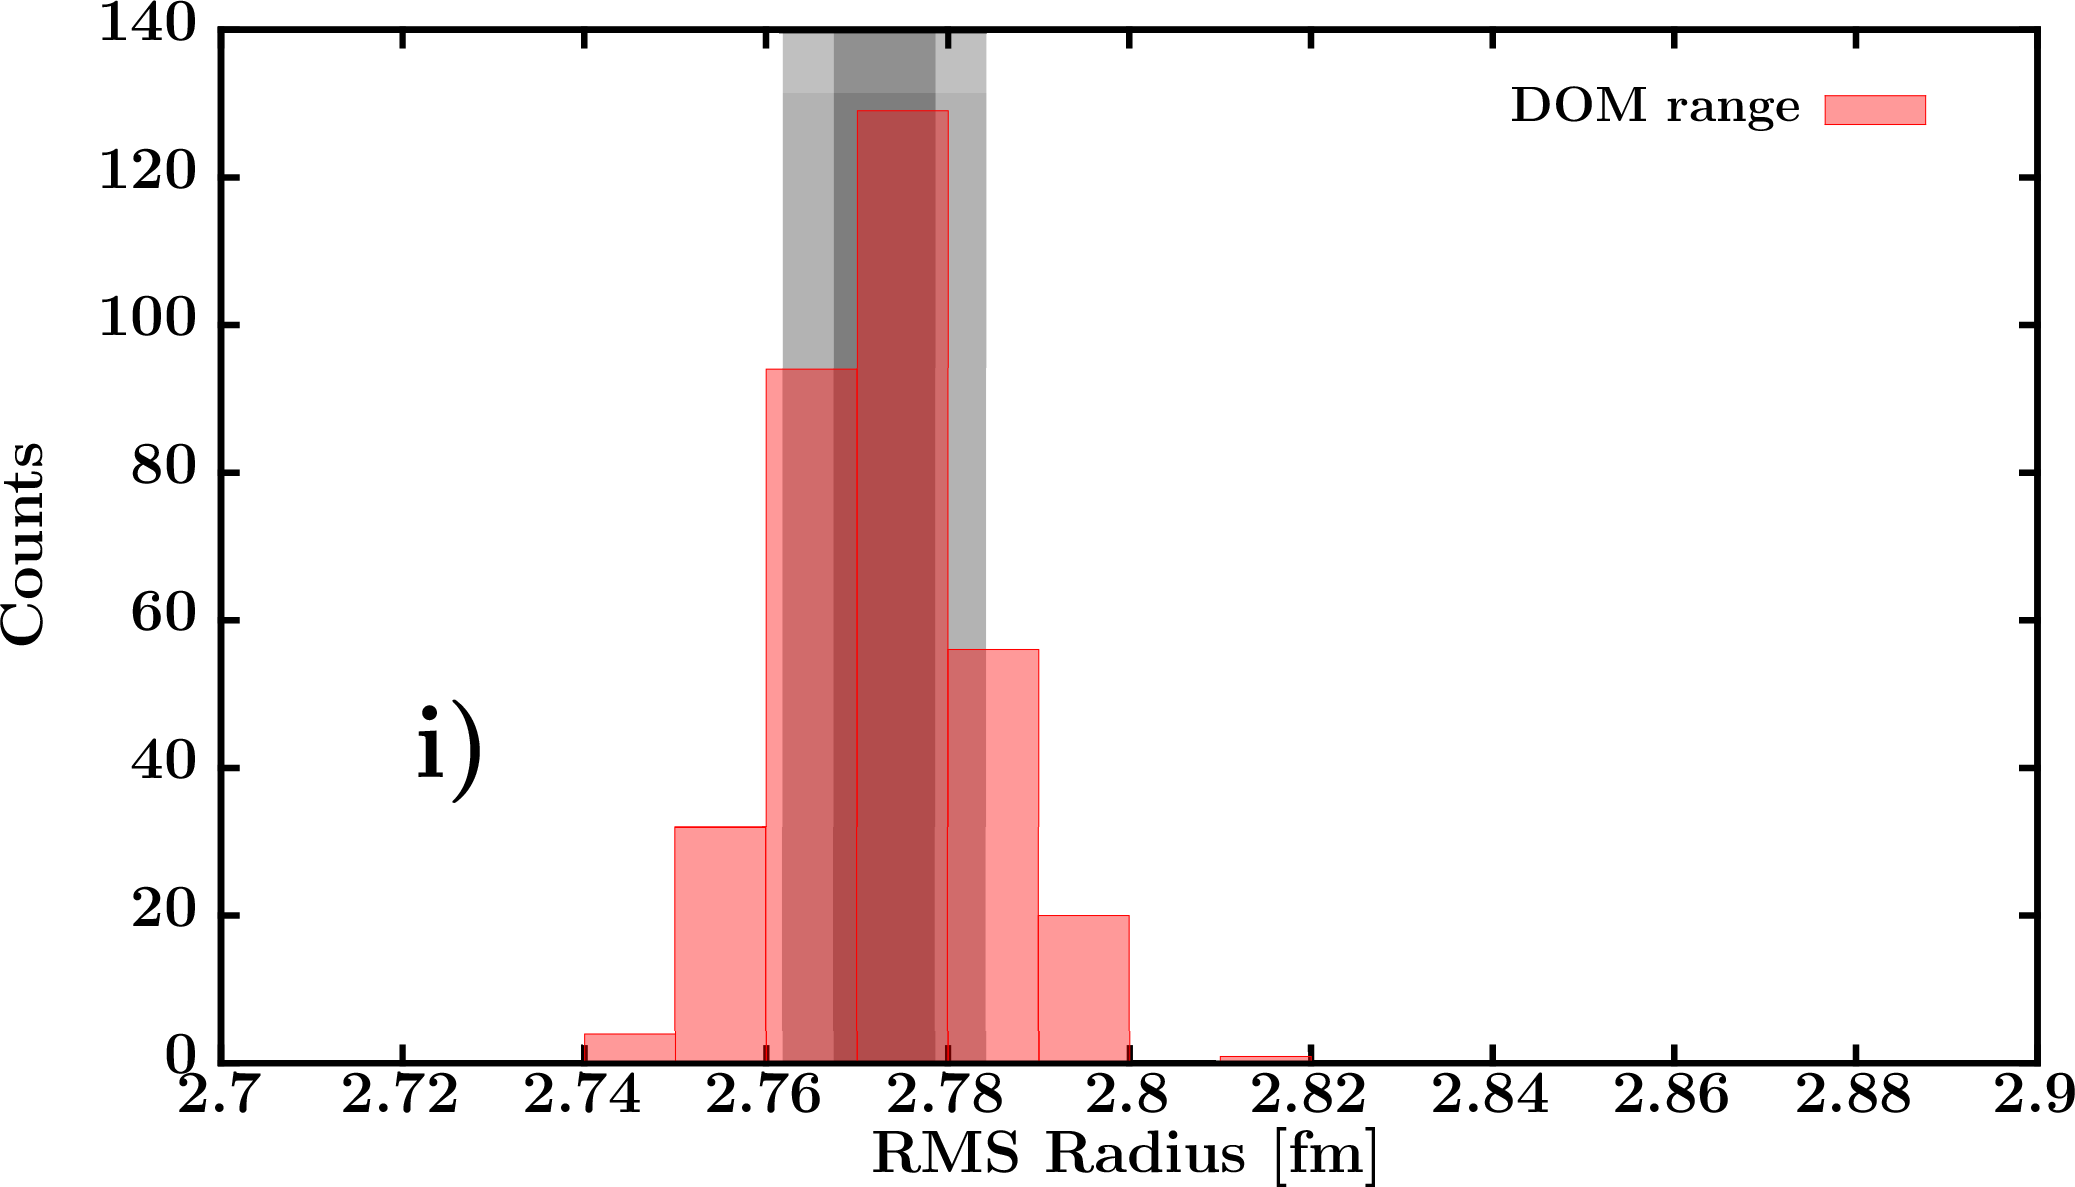
\includegraphics[width=\linewidth]{figures/o18_RMSRadius.png}
        \label{DOM_o18_RMSRadius}
    \end{minipage}
    \begin{minipage}{0.4\linewidth}
        \centering
        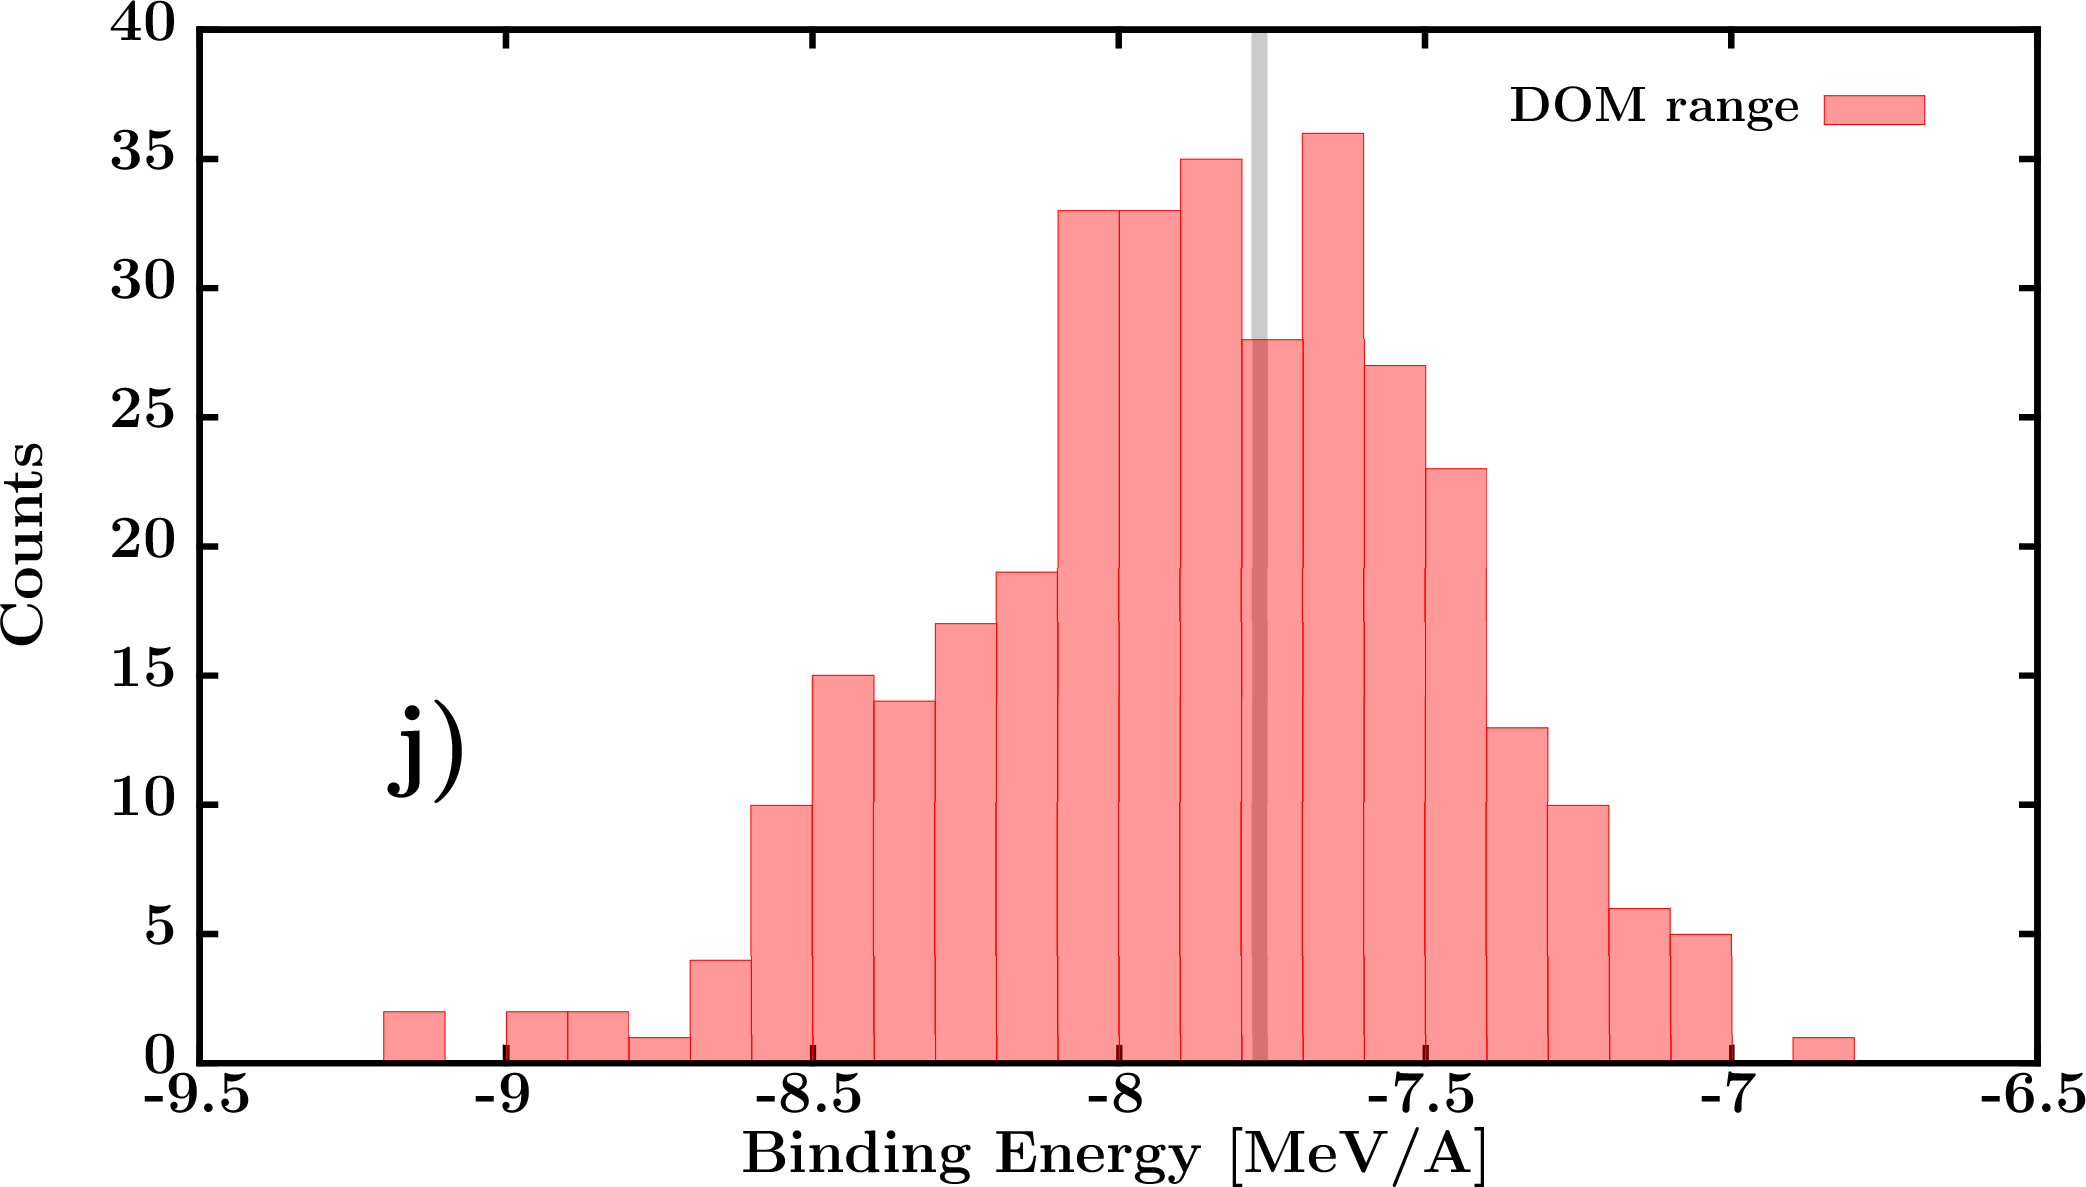
\includegraphics[width=\linewidth]{figures/o18_BE.png}
        \label{DOM_o18_BE}
    \end{minipage}
    \caption{\oEight\ bound-state data used in DOM fit}
    \label{DOM_o18_structural}
\end{figure*}

\begin{figure*}[!htb]
    \centering
    \begin{minipage}{0.4\linewidth}
        \centering
        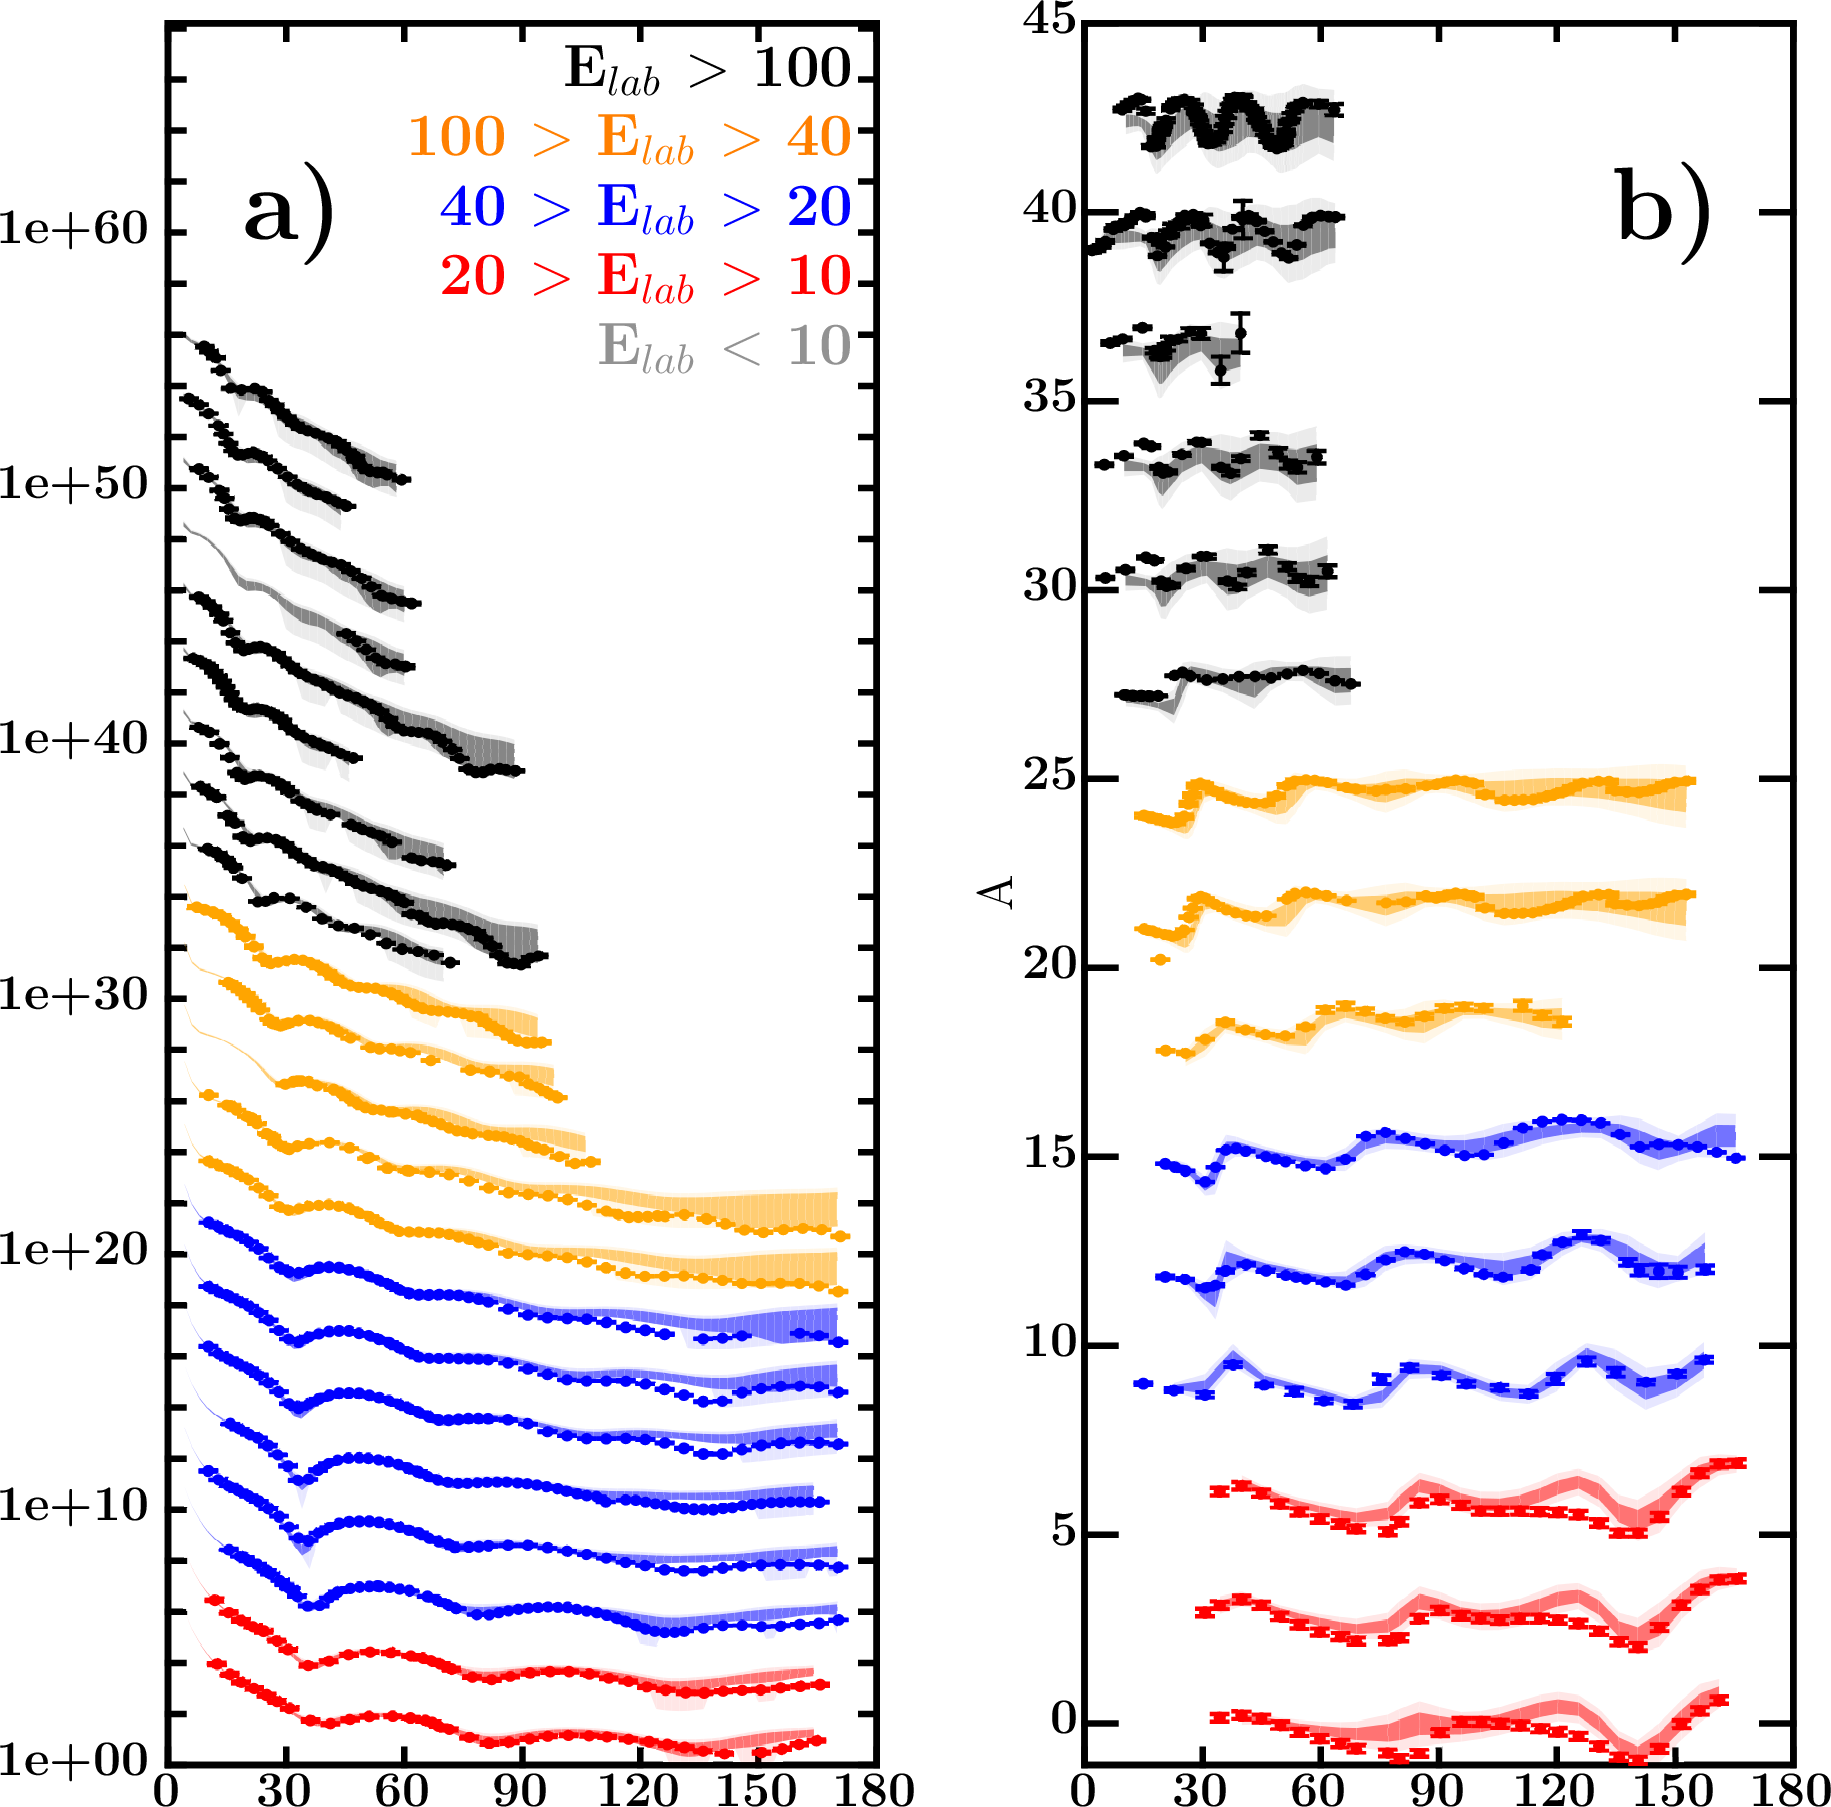
\includegraphics[width=\linewidth]{figures/ca40_protonElastic.png}
        \label{DOM_ca40_proton_elastic}
    \end{minipage}\hspace{6pt}
    \begin{minipage}{0.4\linewidth}
        \centering
        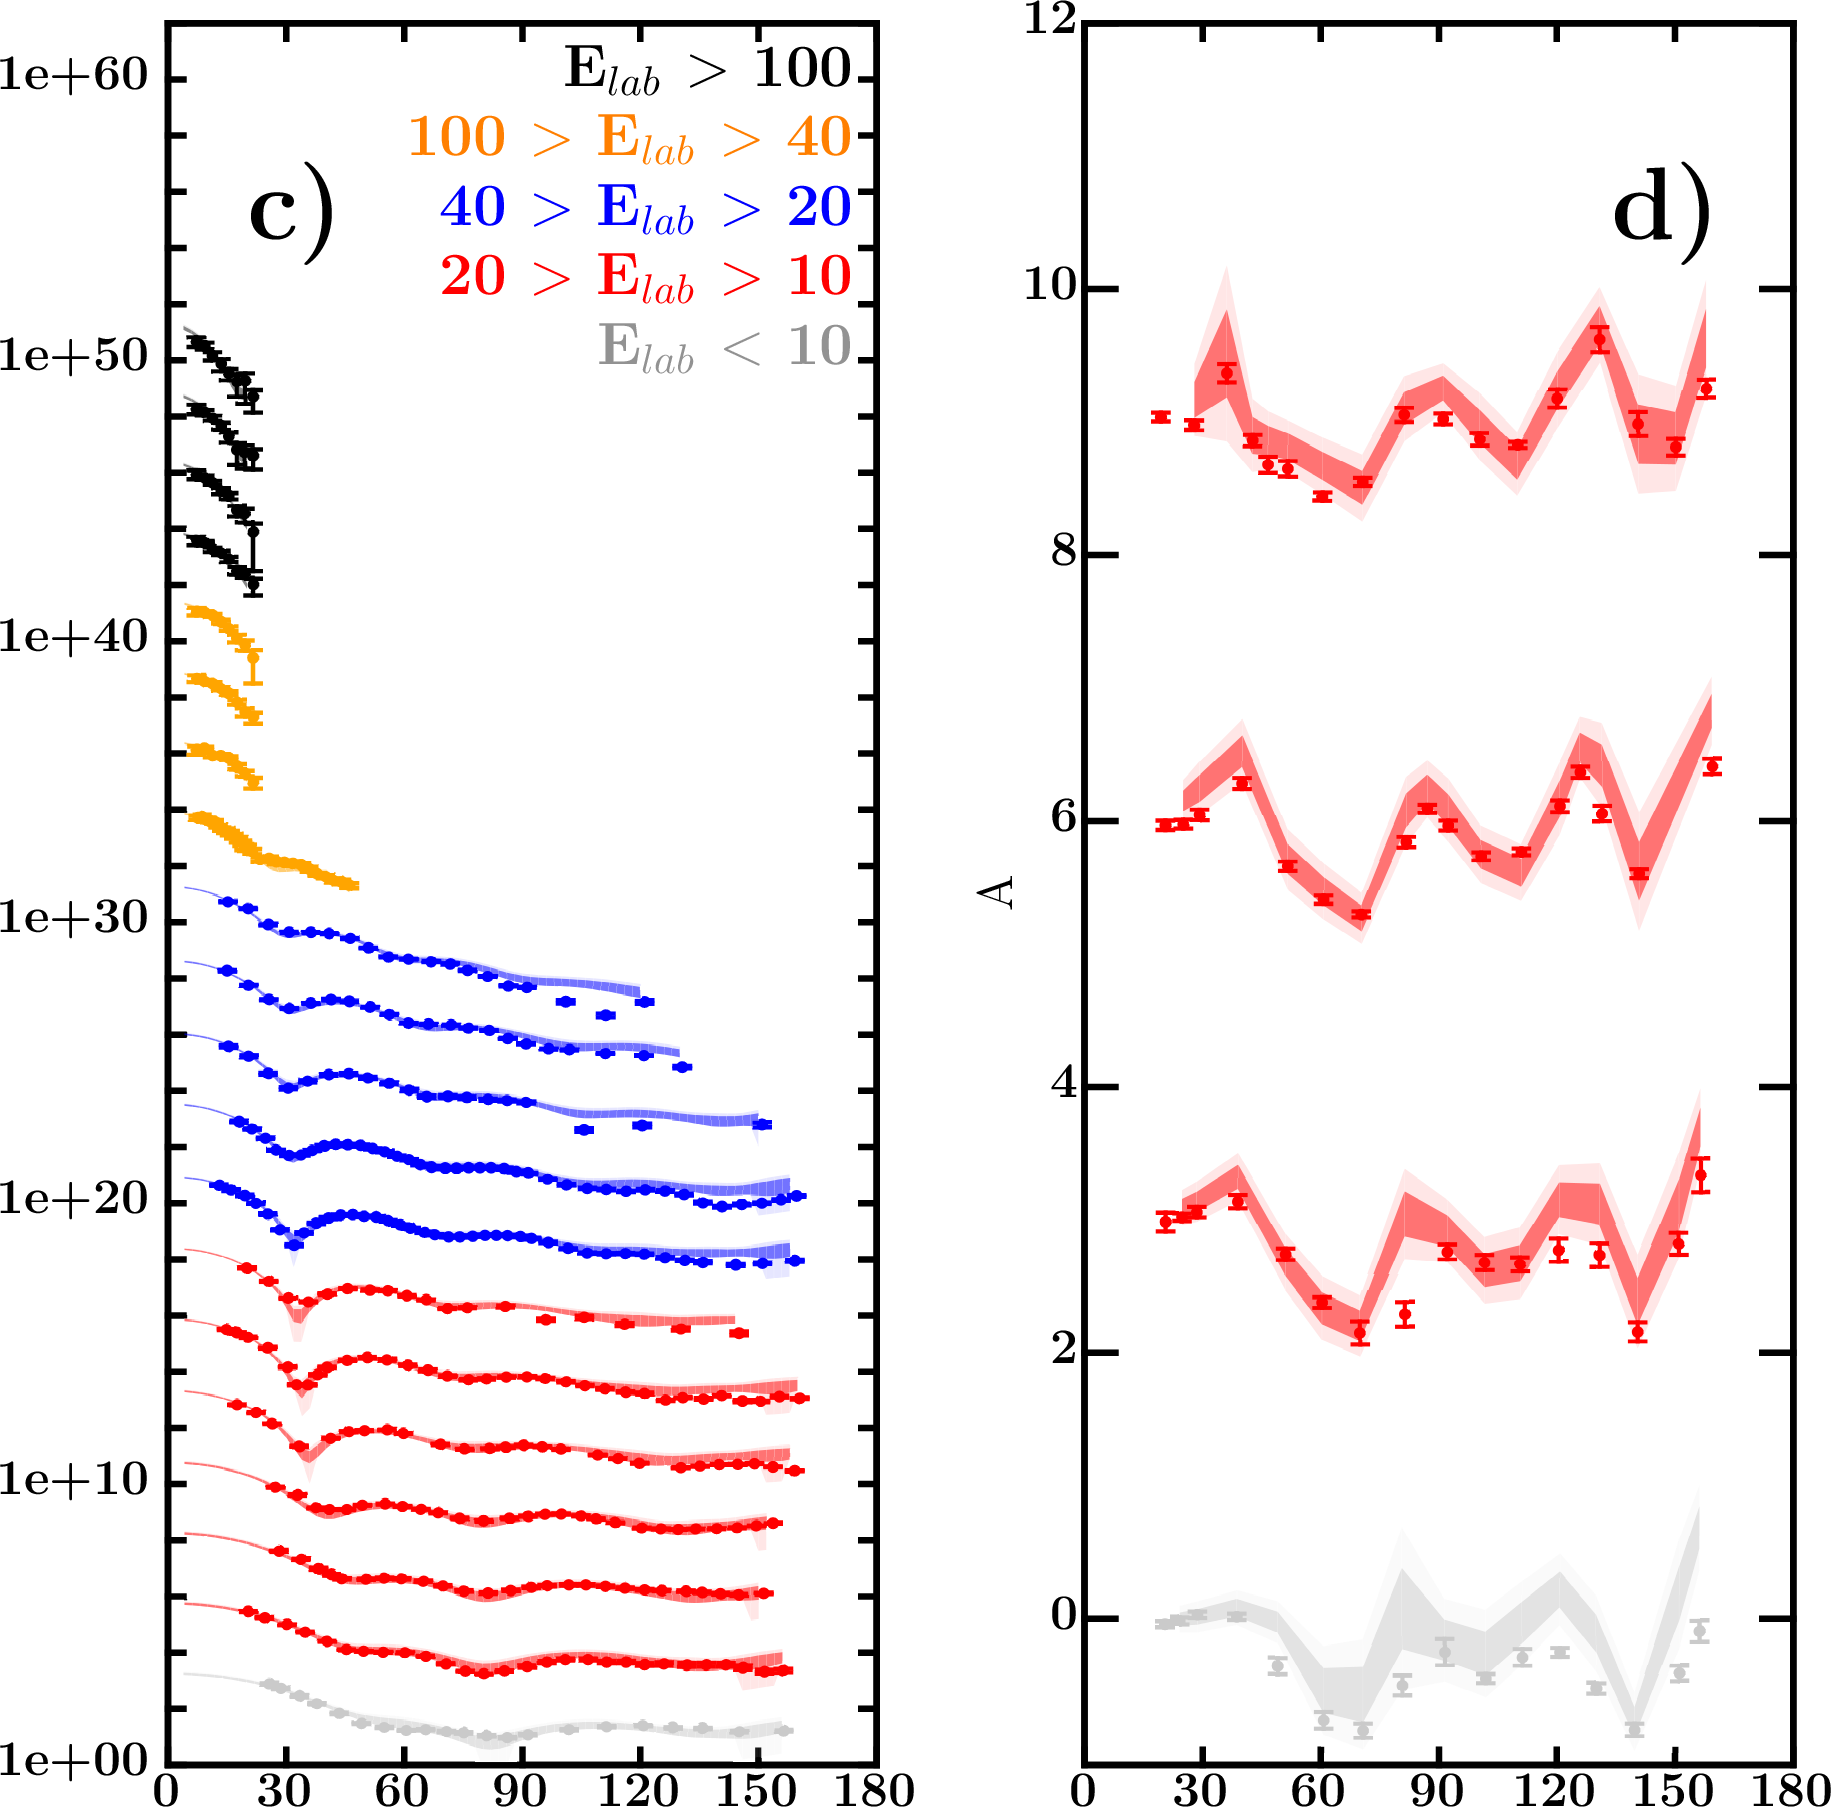
\includegraphics[width=\linewidth]{figures/ca40_neutronElastic.png}
        \label{DOM_ca40_neutron_elastic}
    \end{minipage}
    \centering
    \begin{minipage}{0.4\linewidth}
        \centering
        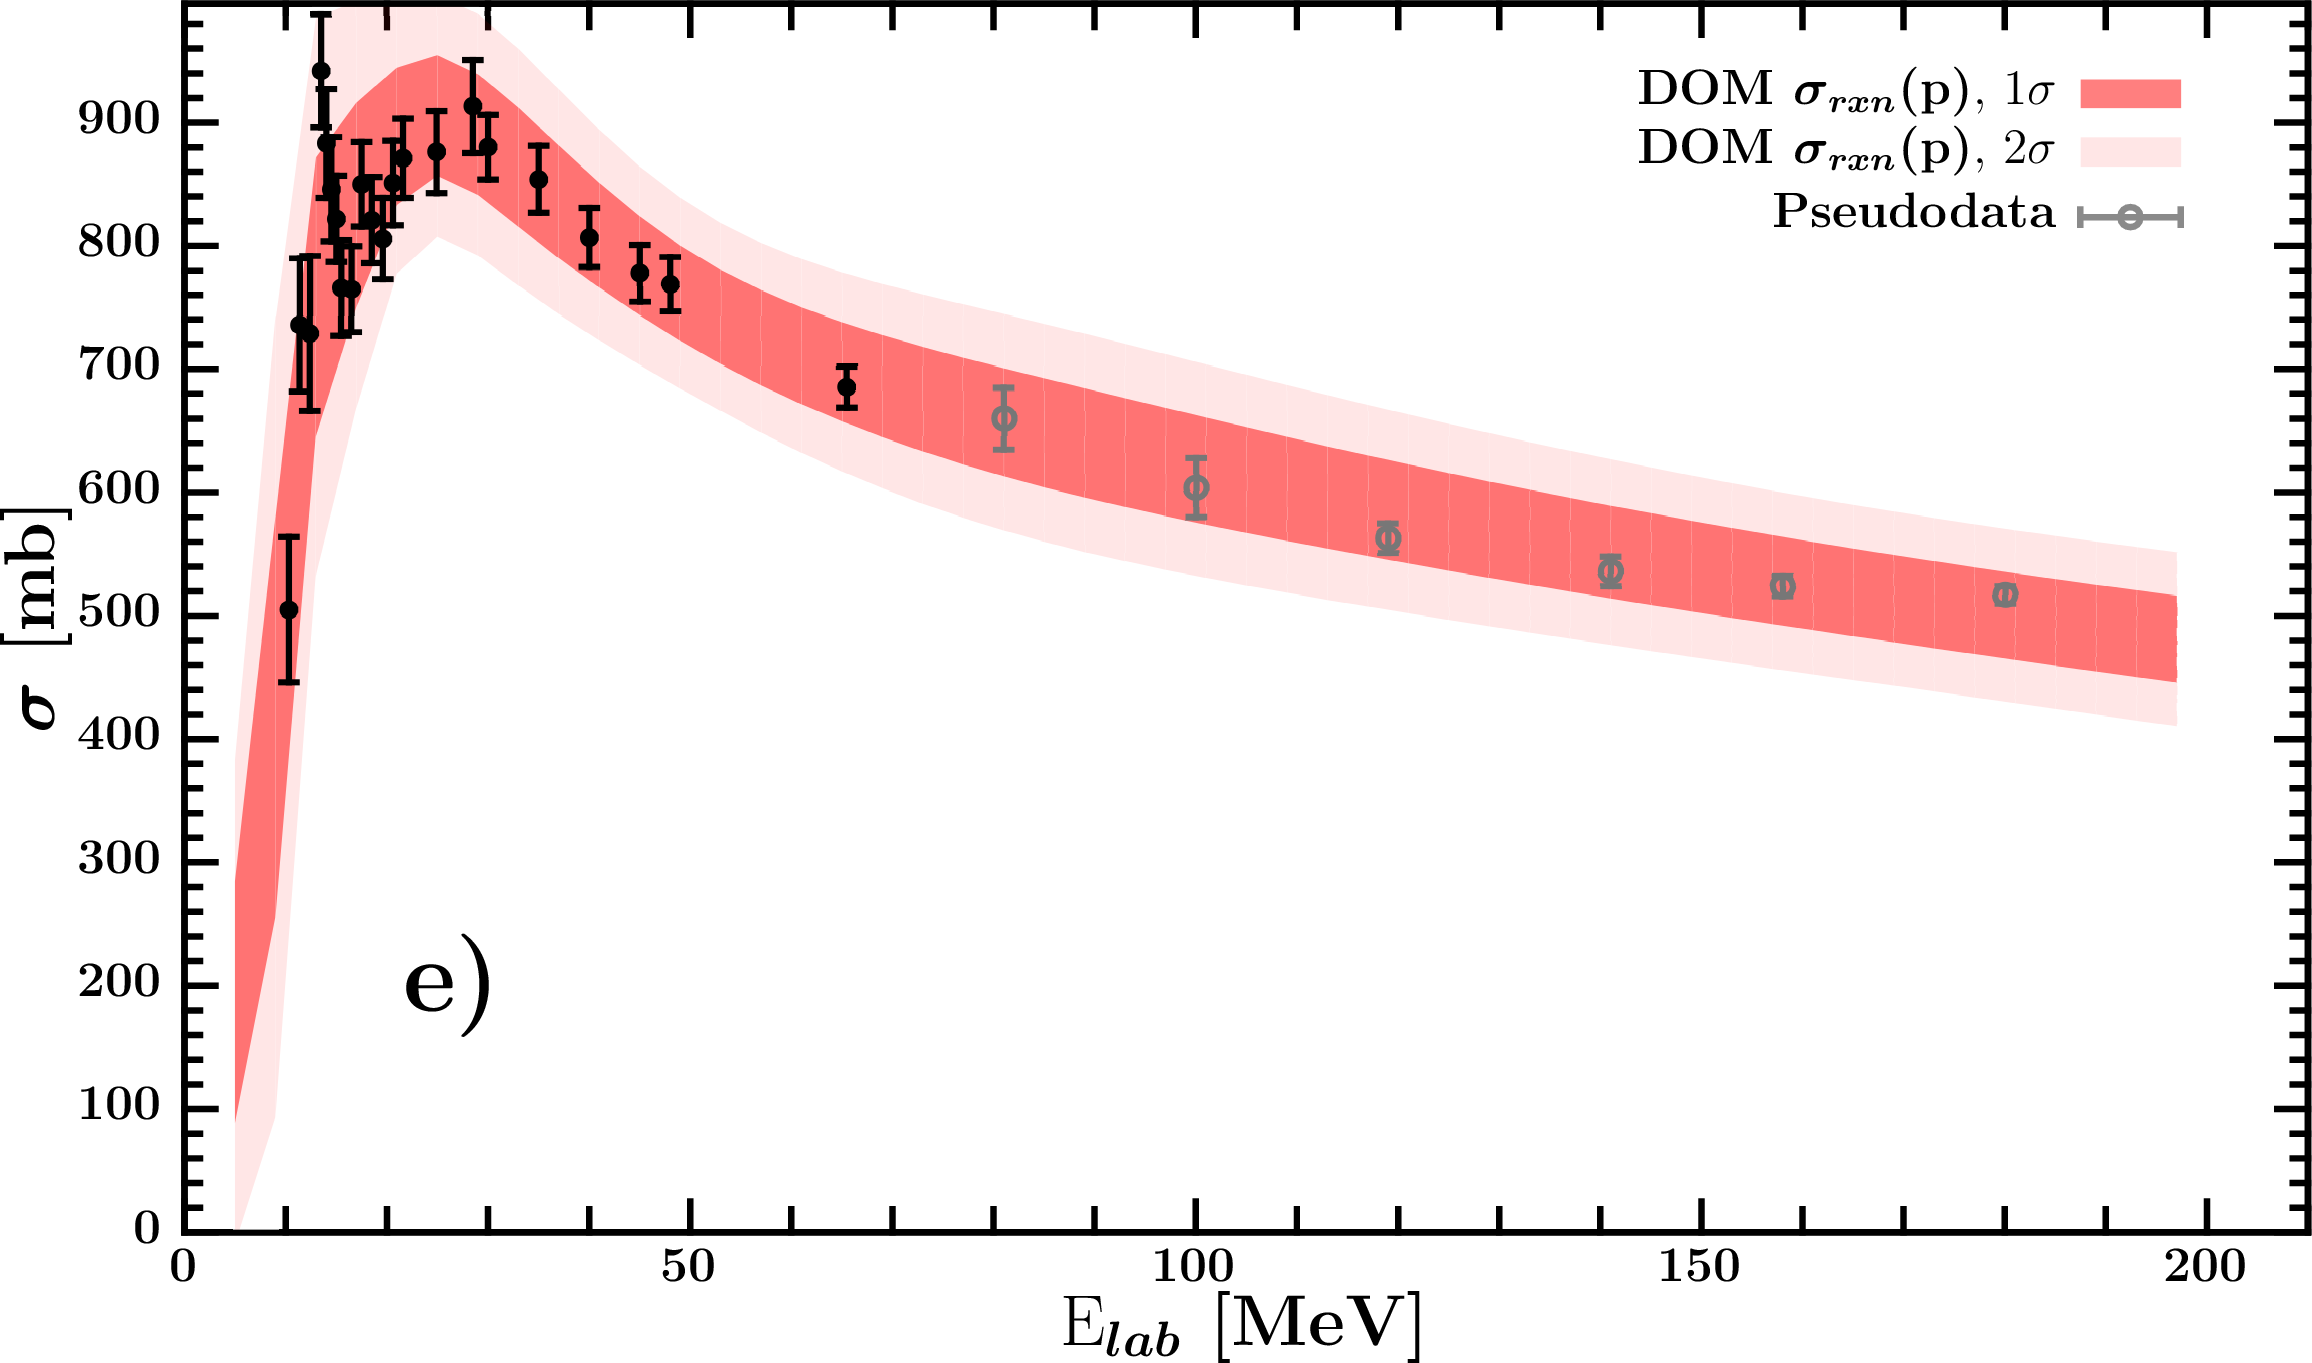
\includegraphics[width=\linewidth]{figures/ca40_protonInelastic.png}
        \label{DOM_ca40_proton_inelastic}
    \end{minipage}\hspace{6pt}
    \begin{minipage}{0.4\linewidth}
        \centering
        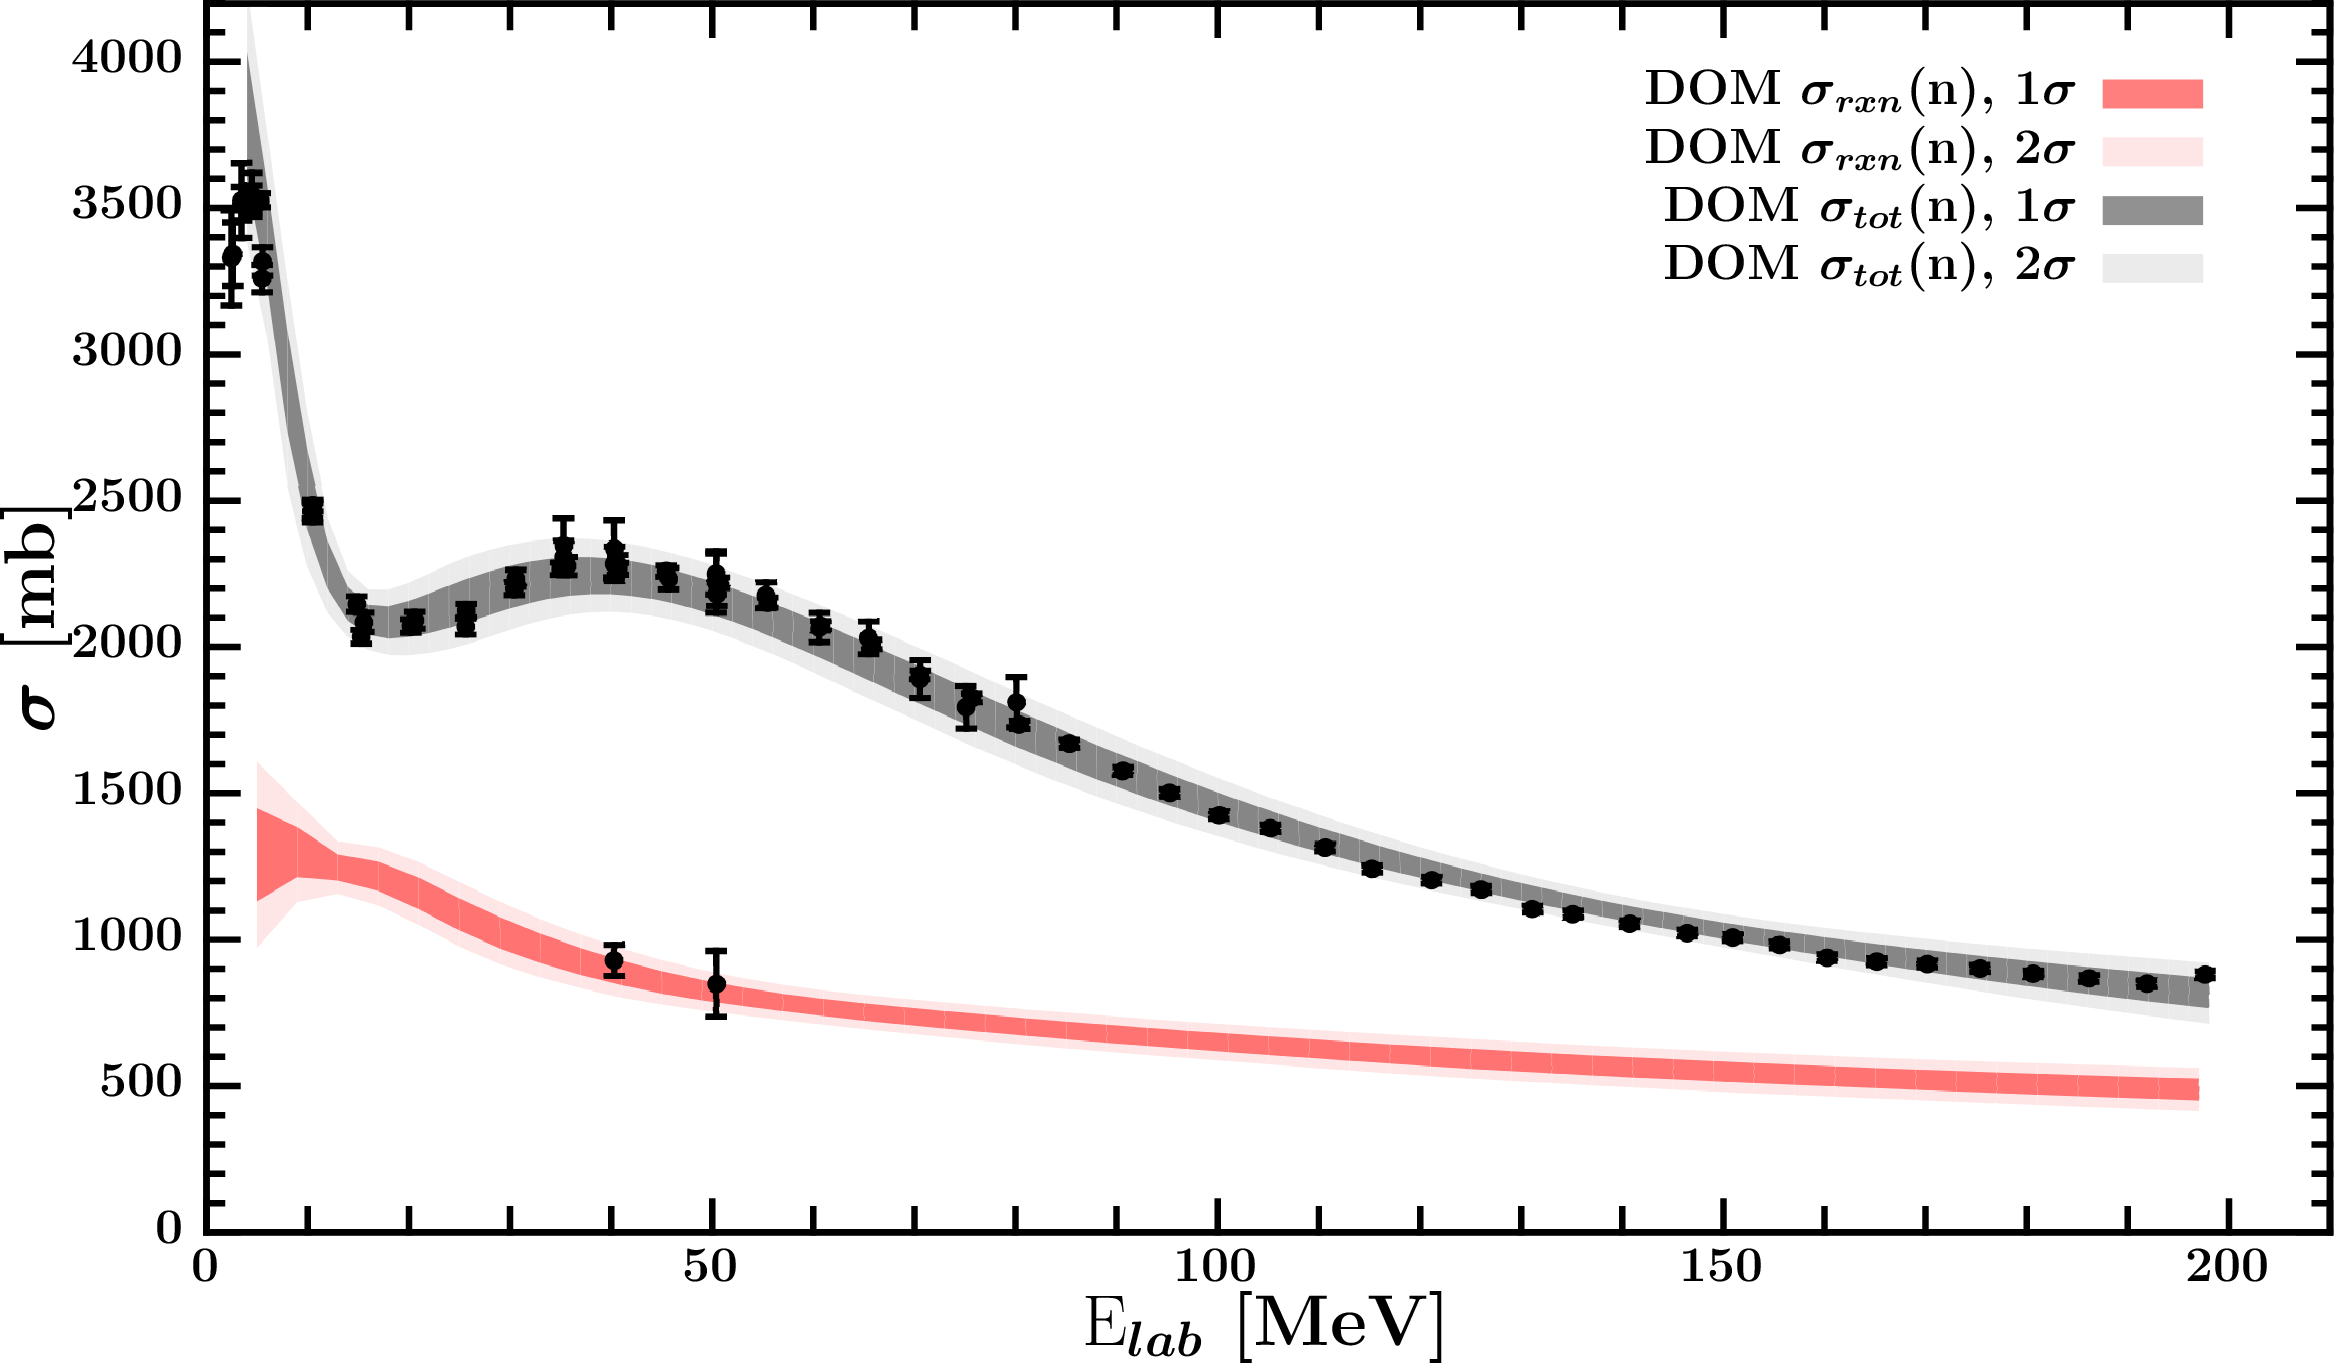
\includegraphics[width=\linewidth]{figures/ca40_neutronInelastic.png}
        \label{DOM_ca40_neutron_inelastic}
    \end{minipage}
    \caption{\caForty\ nucleon scattering data used in DOM fit}
    \label{DOM_ca40_scattering}
    \centering
    \begin{minipage}{0.4\linewidth}
        \centering
        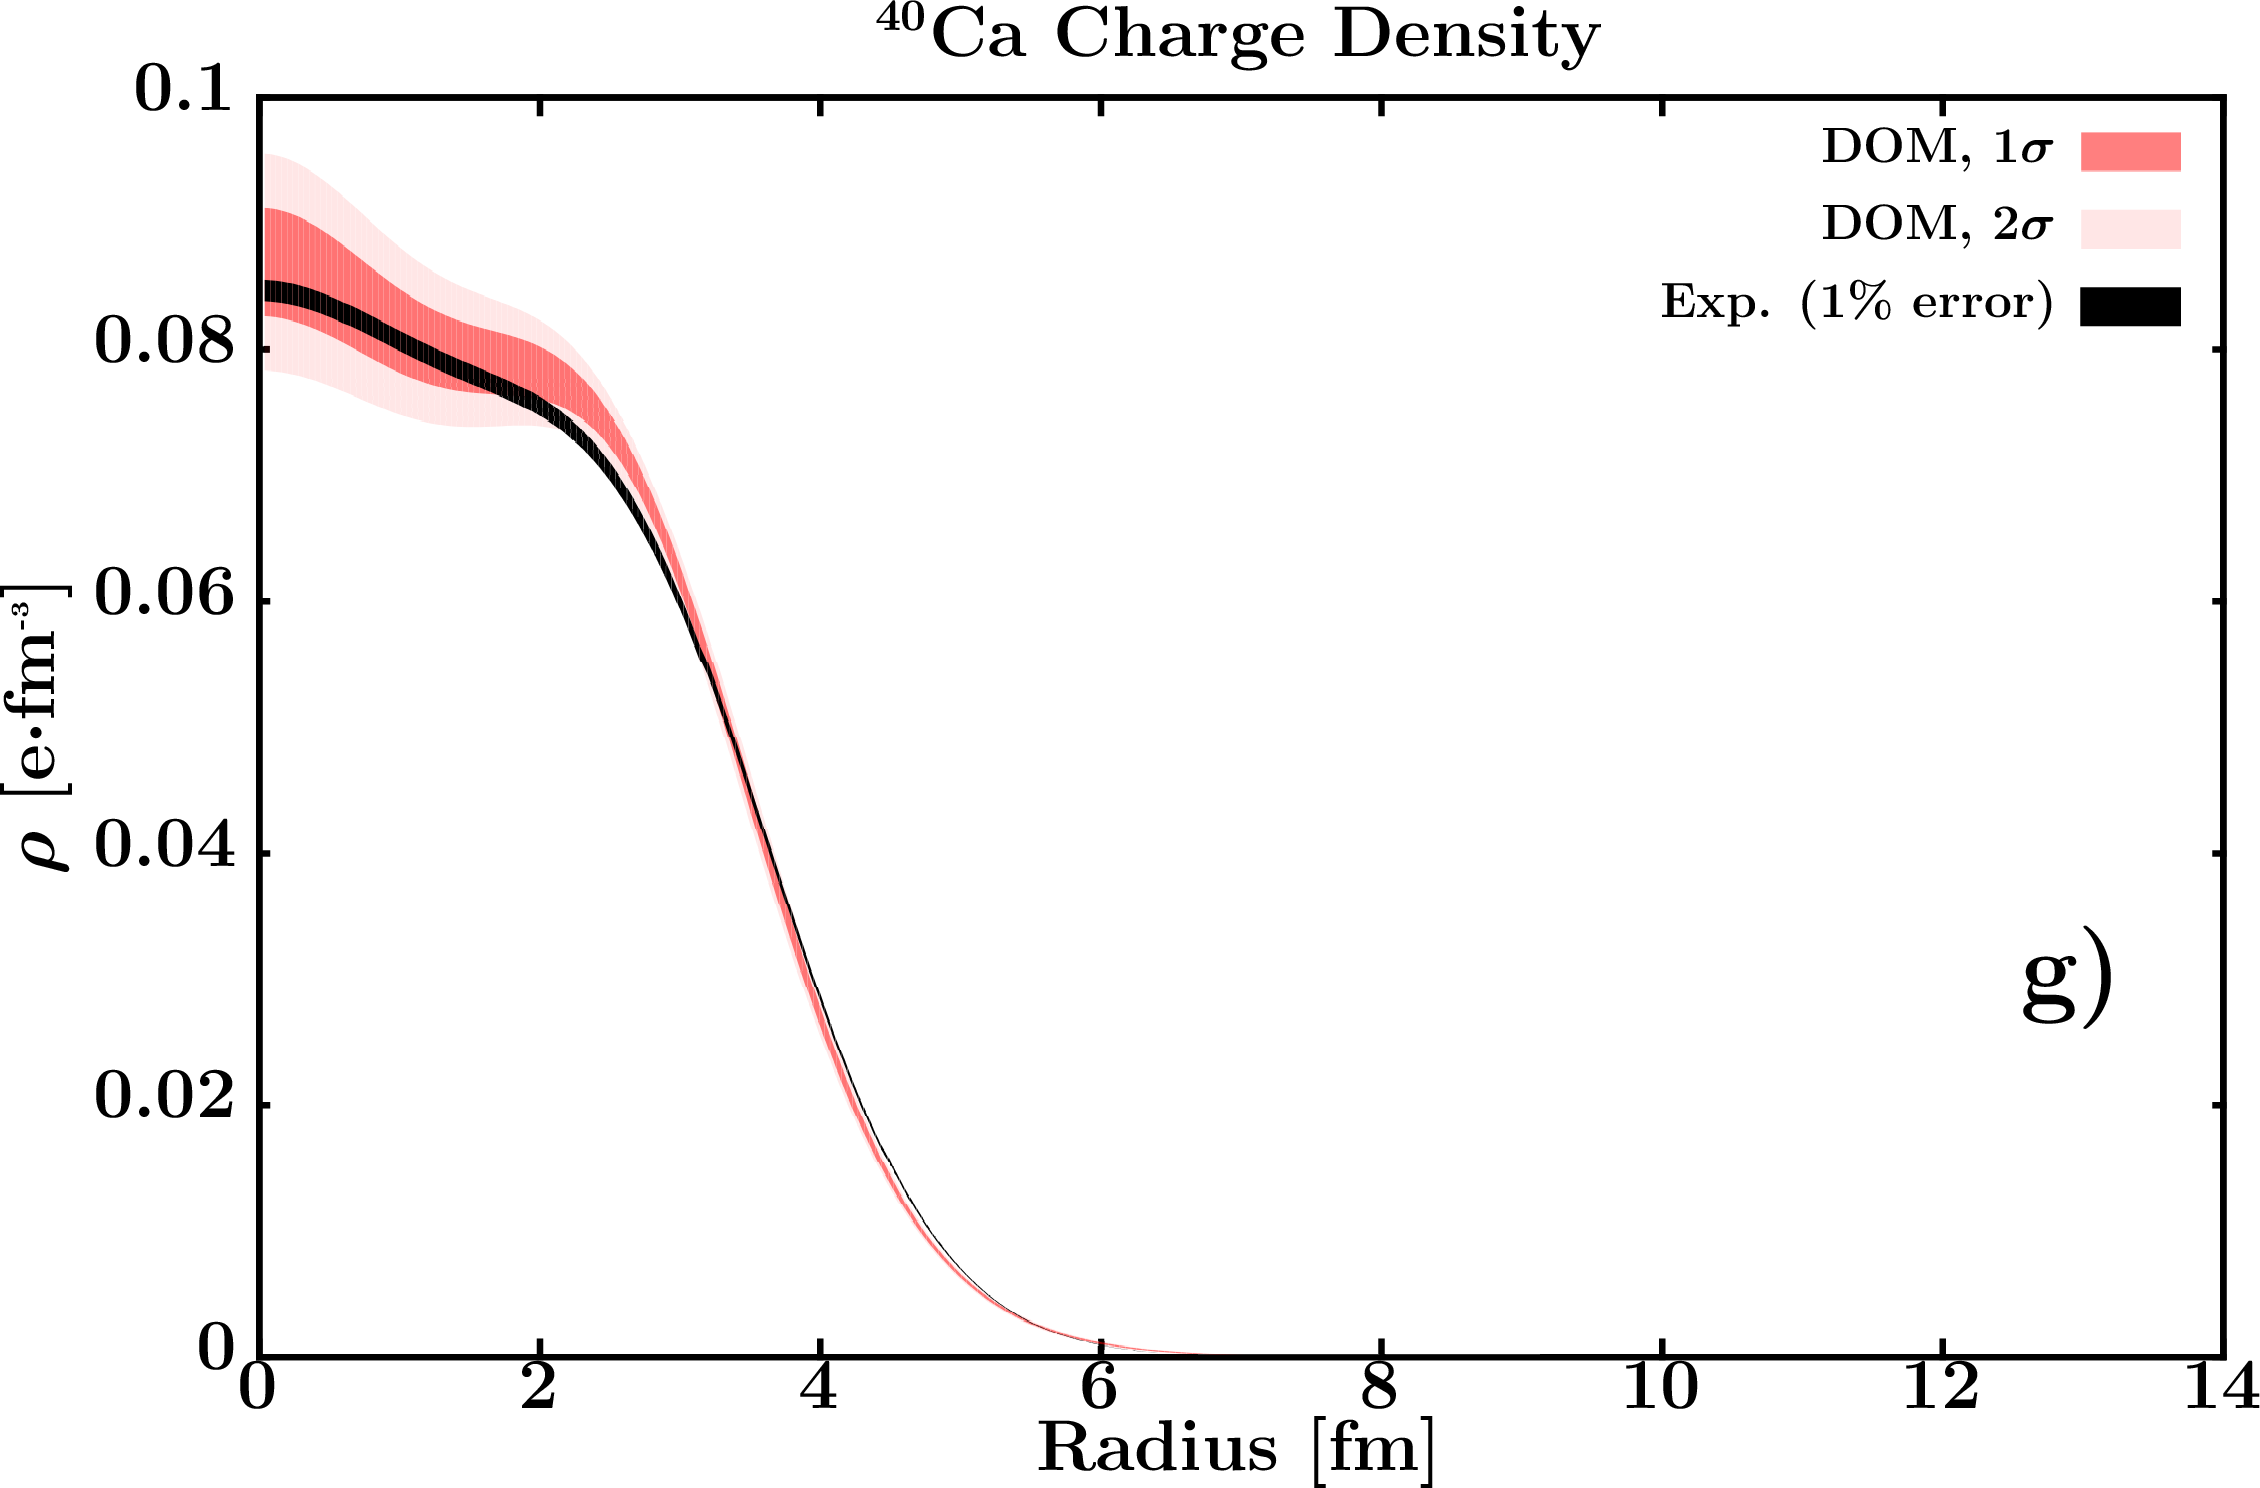
\includegraphics[width=\linewidth]{figures/ca40_chargeDensity.png}
        \label{DOM_ca40_chargeDensity}
    \end{minipage}
    \begin{minipage}{0.35\linewidth}
        \centering
        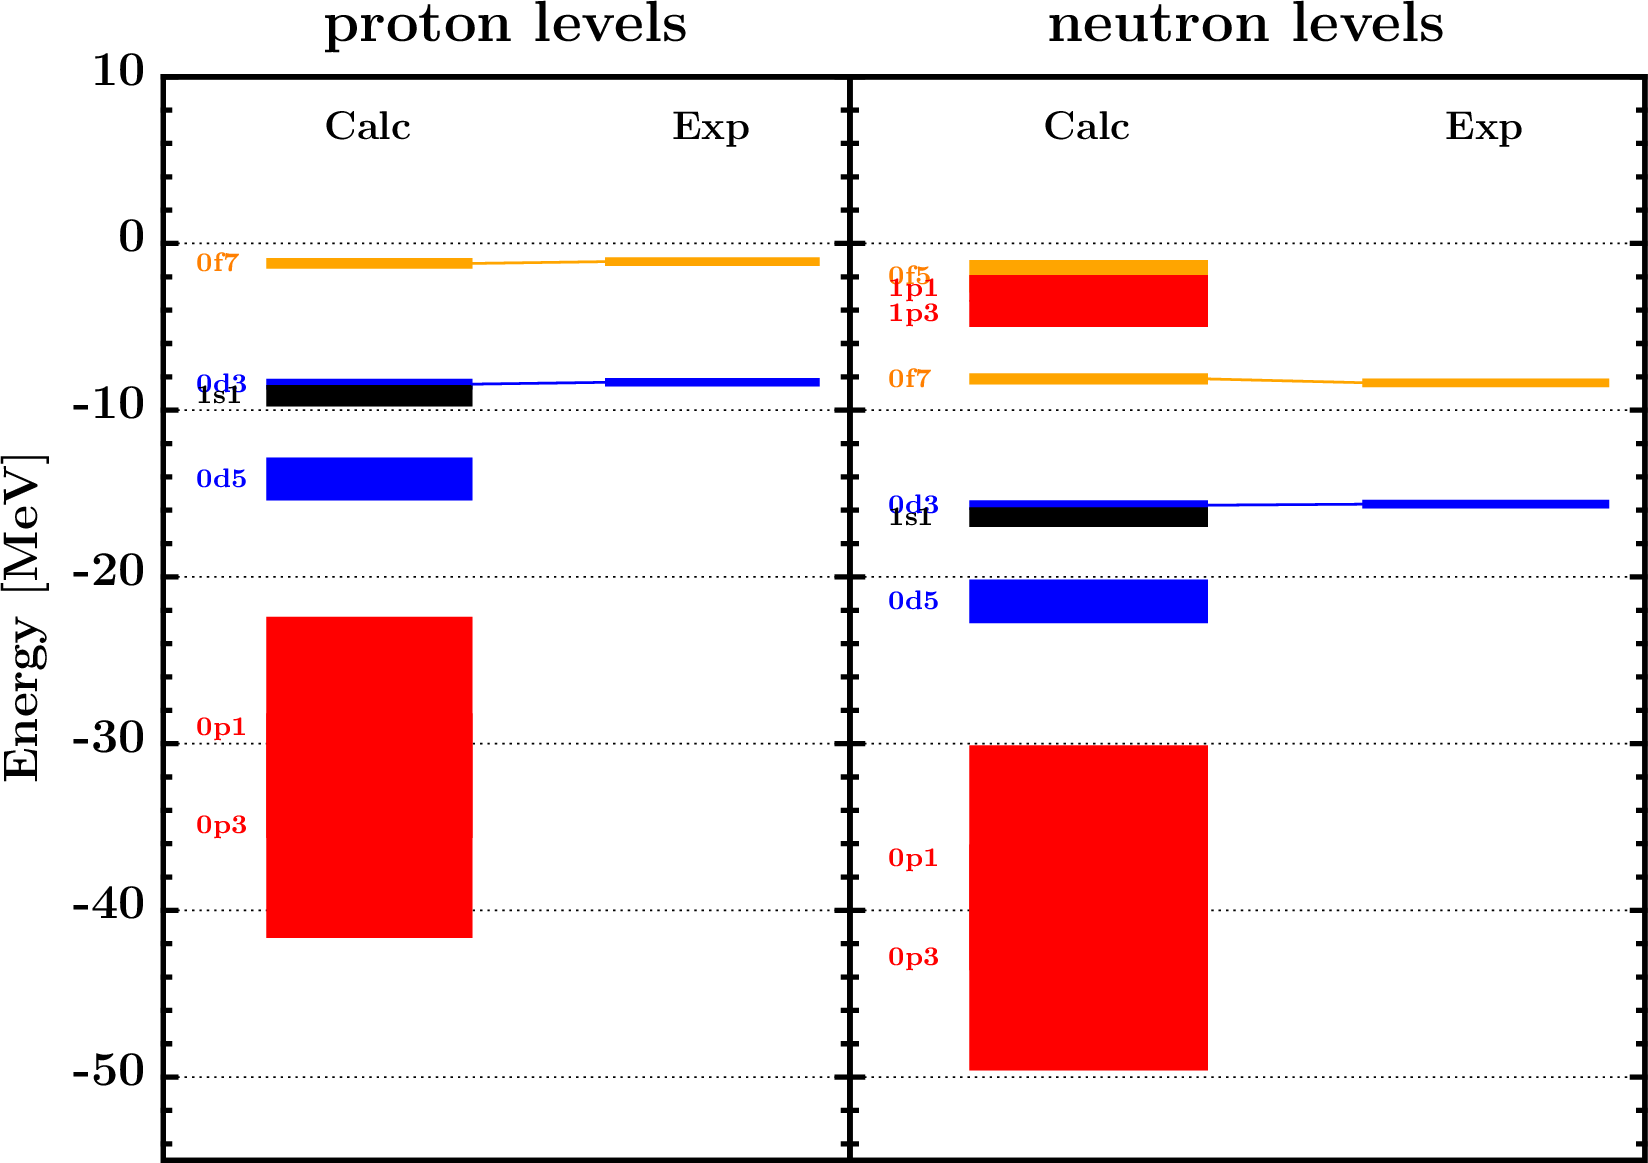
\includegraphics[width=\linewidth]{figures/ca40_SPLevels.png}
        \label{DOM_ca40_SPLevels}
    \end{minipage}
    \begin{minipage}{0.4\linewidth}
        \centering
        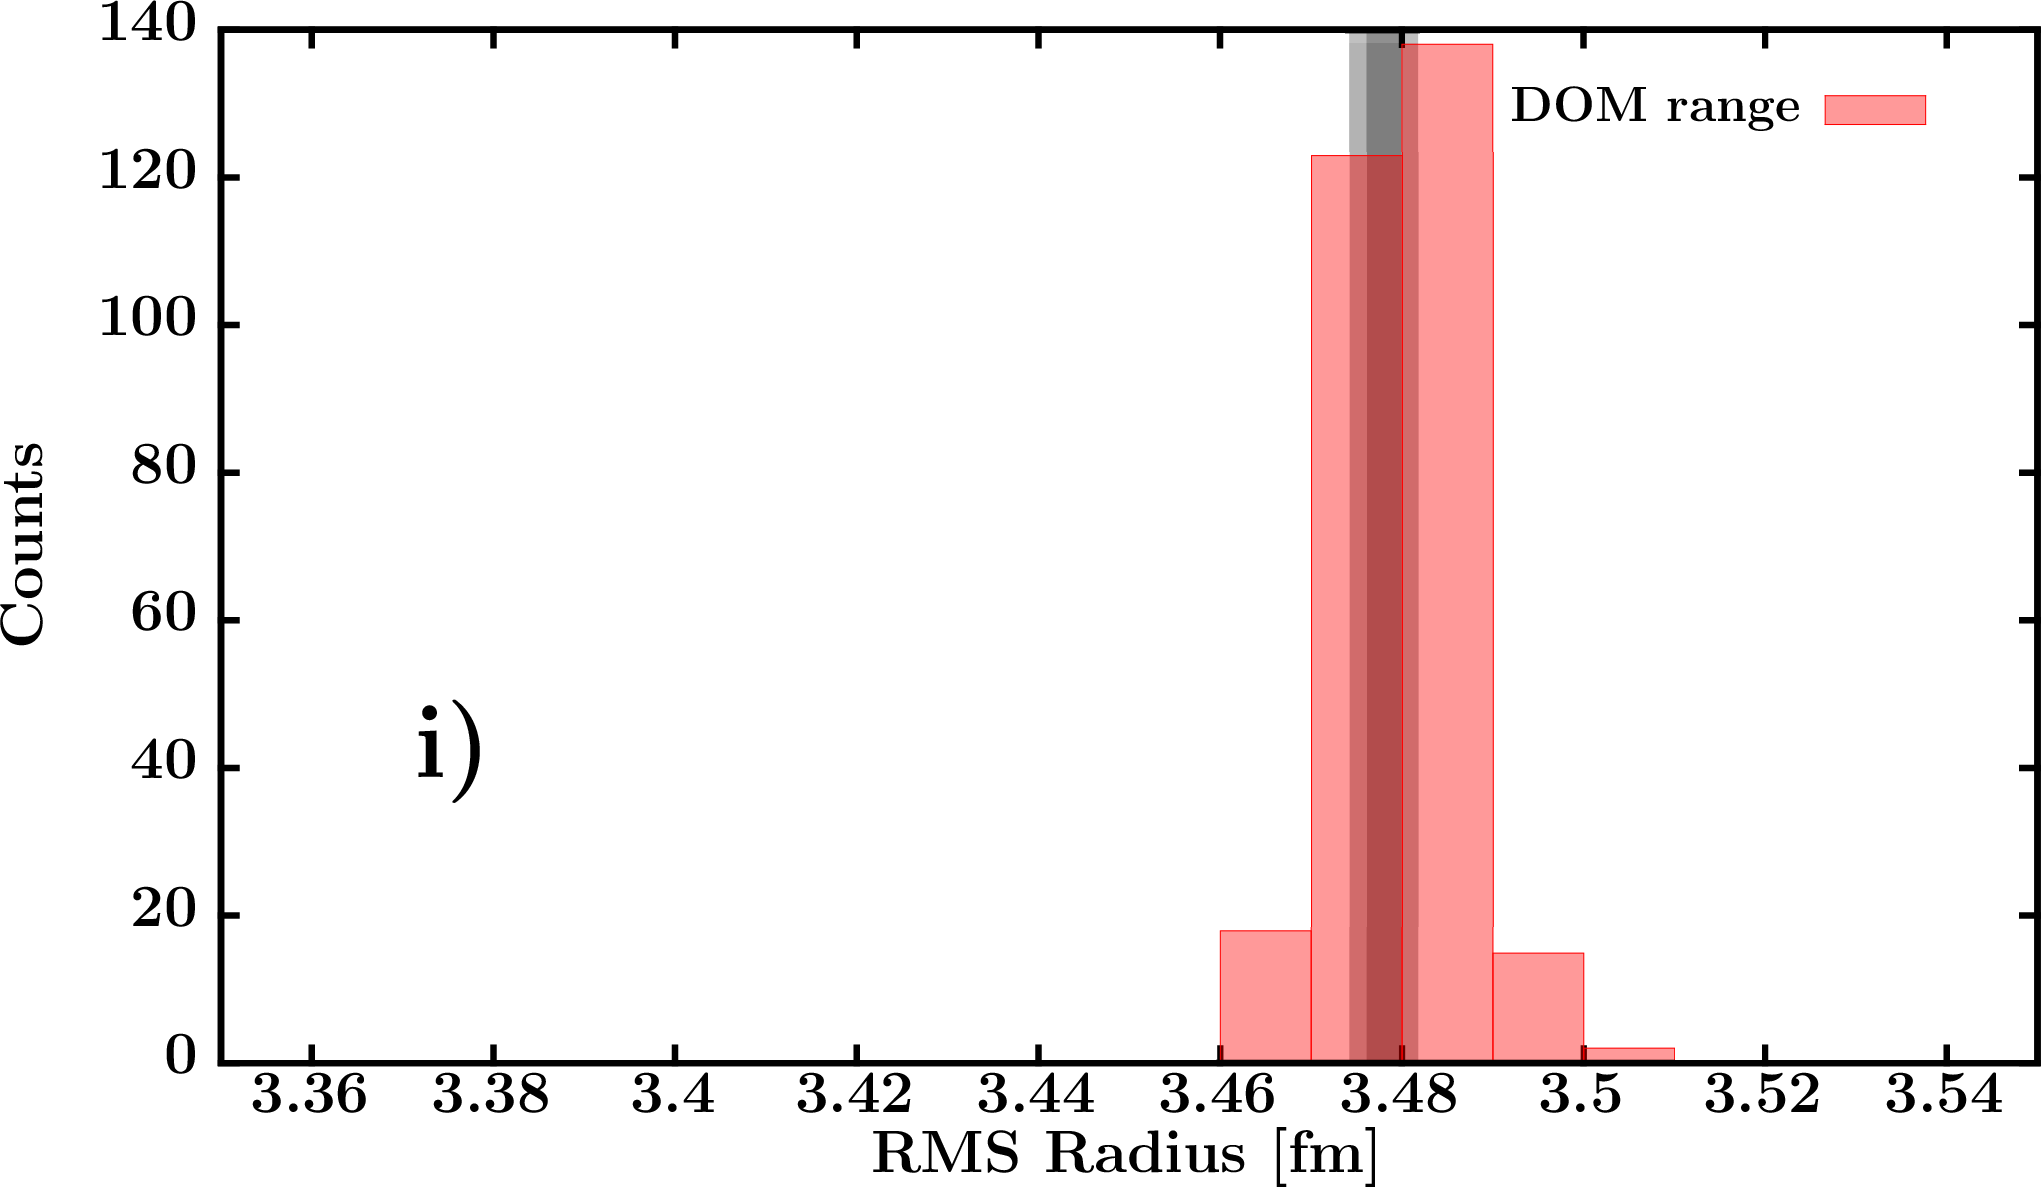
\includegraphics[width=\linewidth]{figures/ca40_RMSRadius.png}
        \label{DOM_ca40_RMSRadius}
    \end{minipage}
    \begin{minipage}{0.4\linewidth}
        \centering
        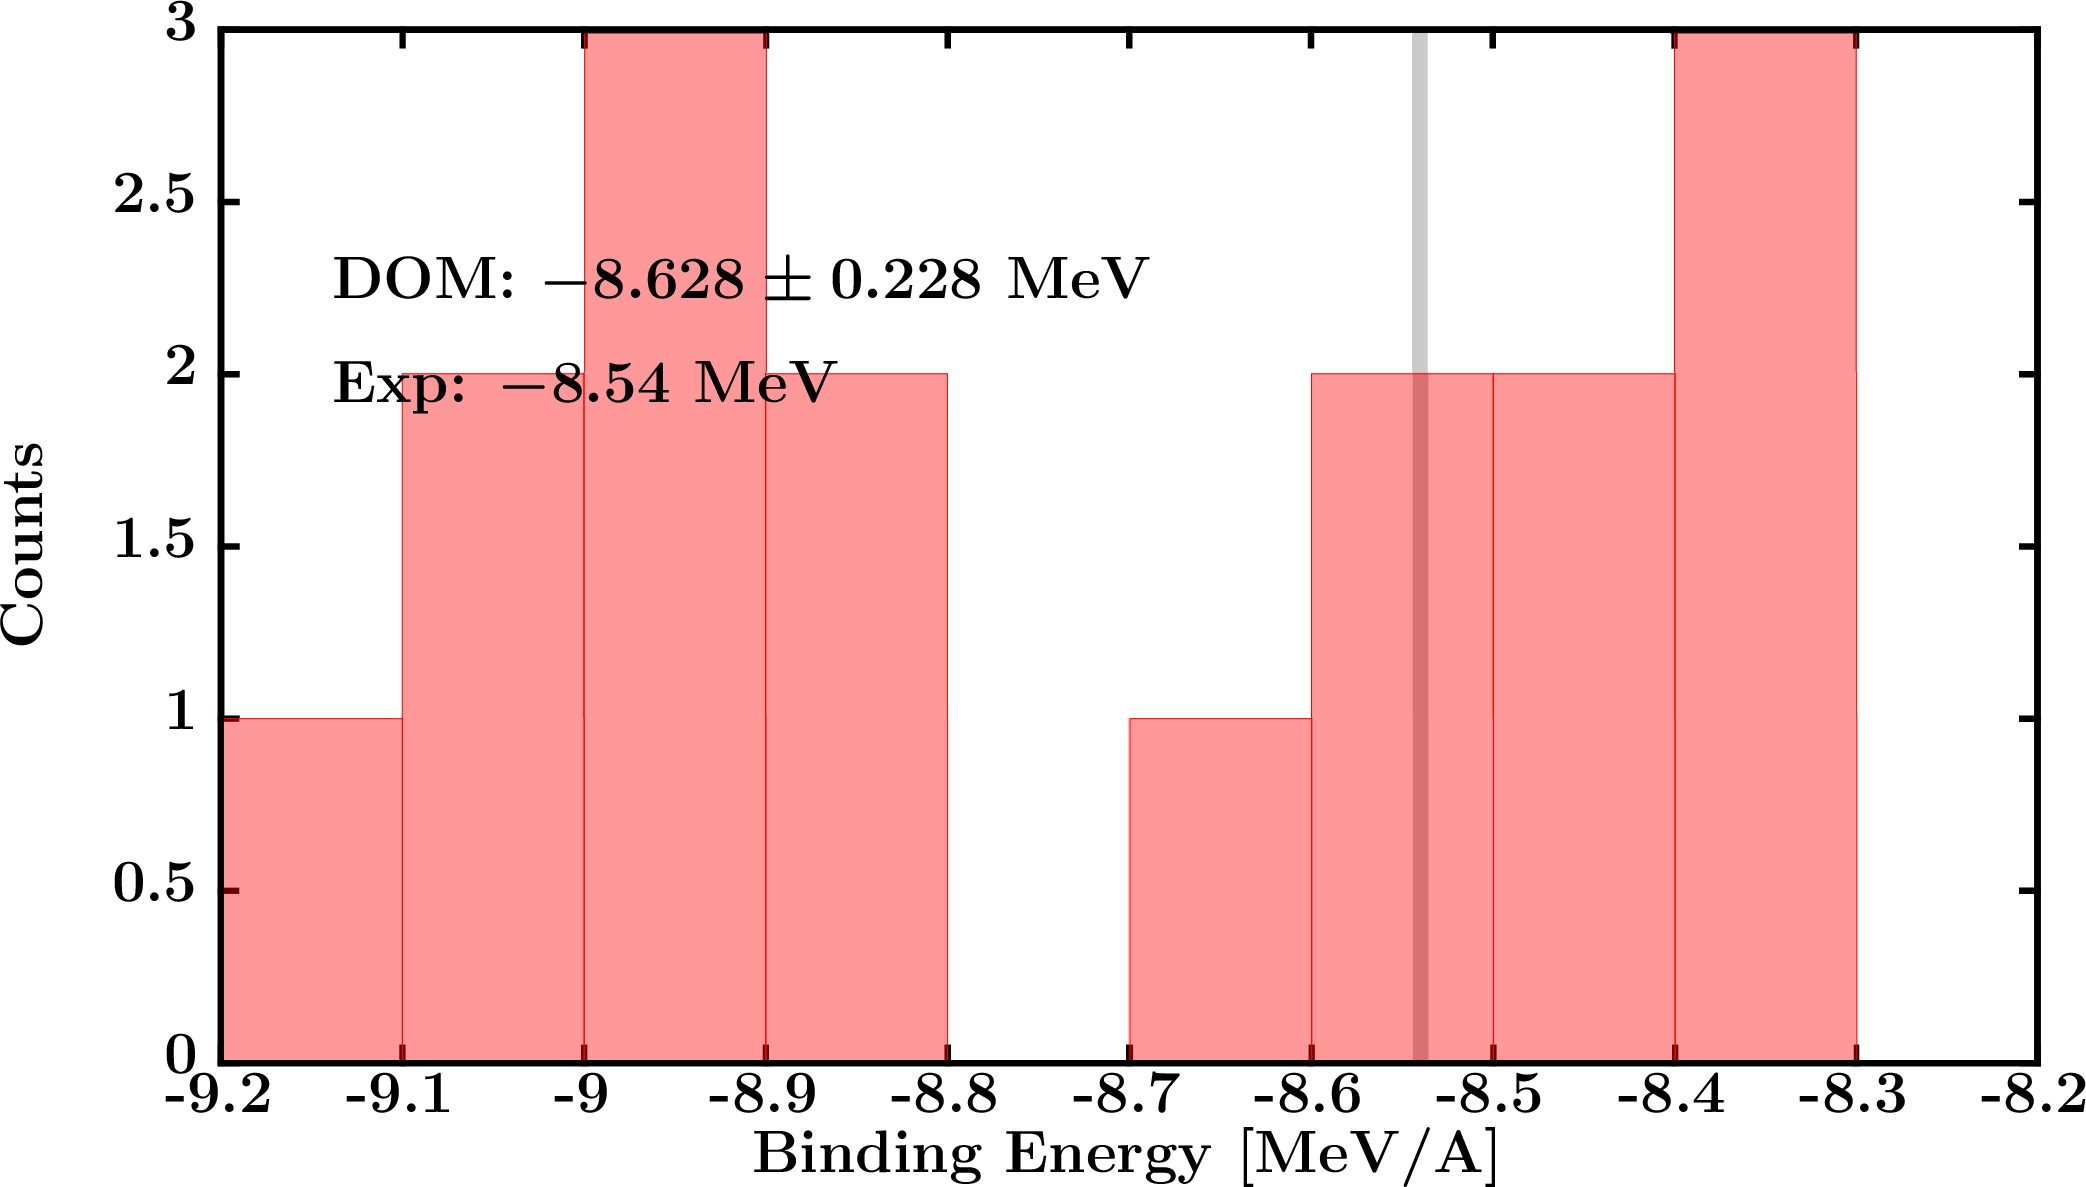
\includegraphics[width=\linewidth]{figures/ca40_BE.png}
        \label{DOM_ca40_BE}
    \end{minipage}
    \caption{\caForty\ bound-state data used in DOM fit}
    \label{DOM_ca40_structural}
\end{figure*}

\begin{figure*}[!htb]
    \centering
    \begin{minipage}{0.4\linewidth}
        \centering
        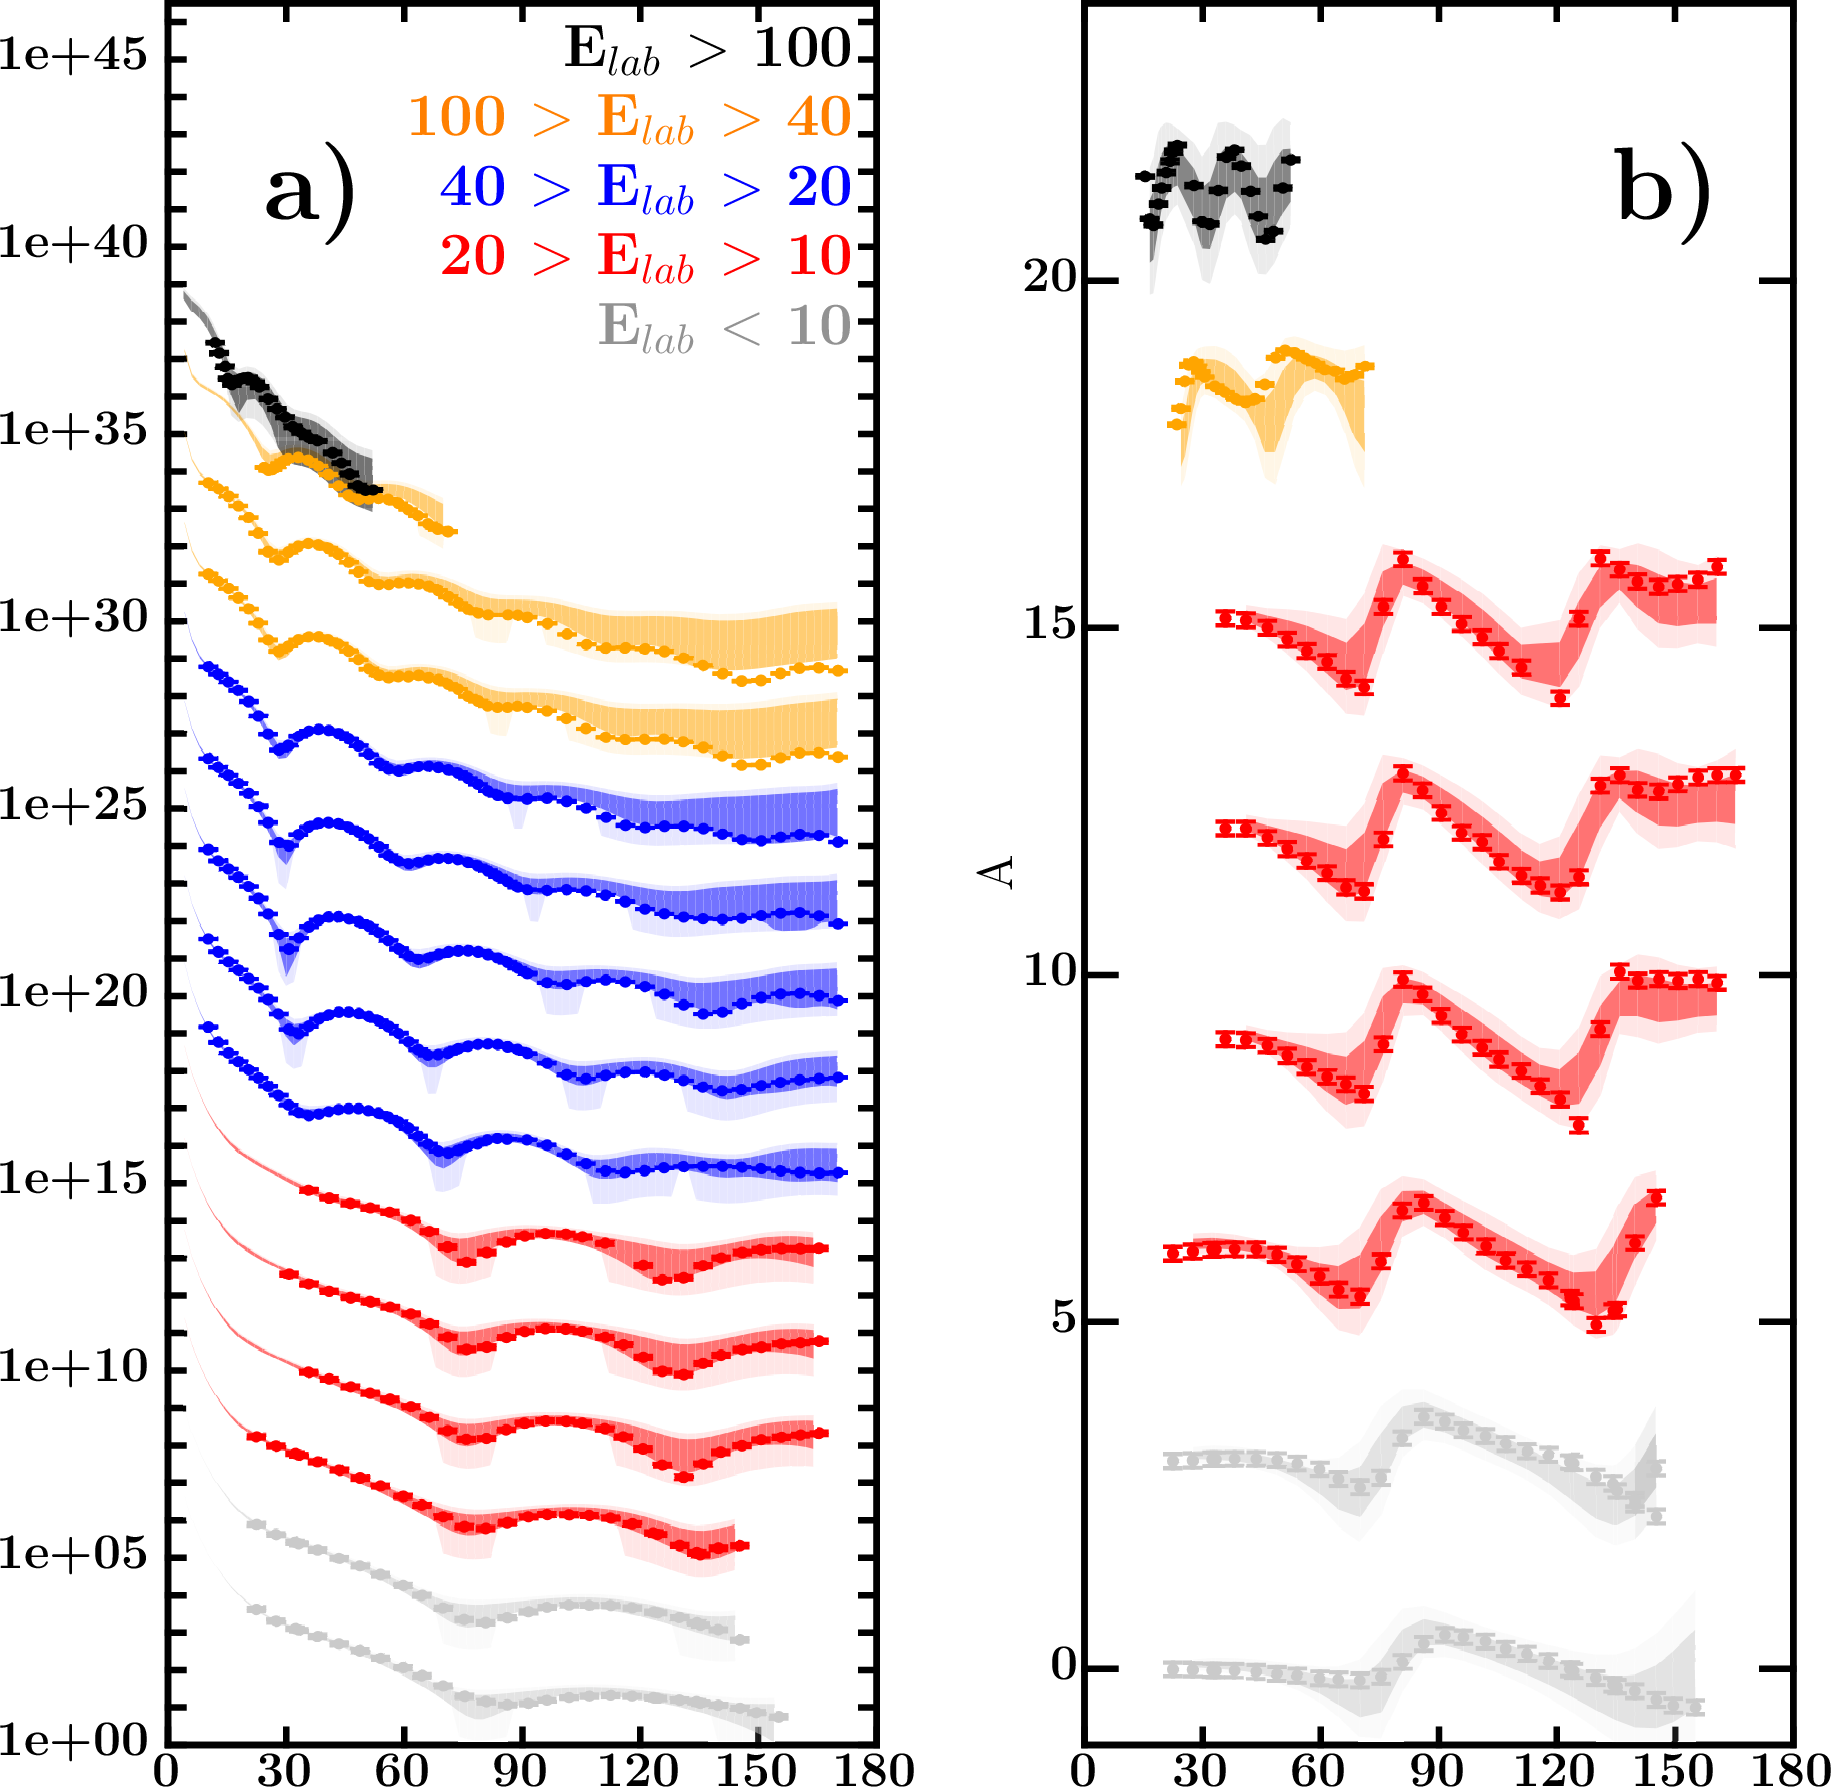
\includegraphics[width=\linewidth]{figures/ca48_protonElastic.png}
        \label{DOM_ca48_proton_elastic}
    \end{minipage}\hspace{6pt}
    \begin{minipage}{0.4\linewidth}
        \centering
        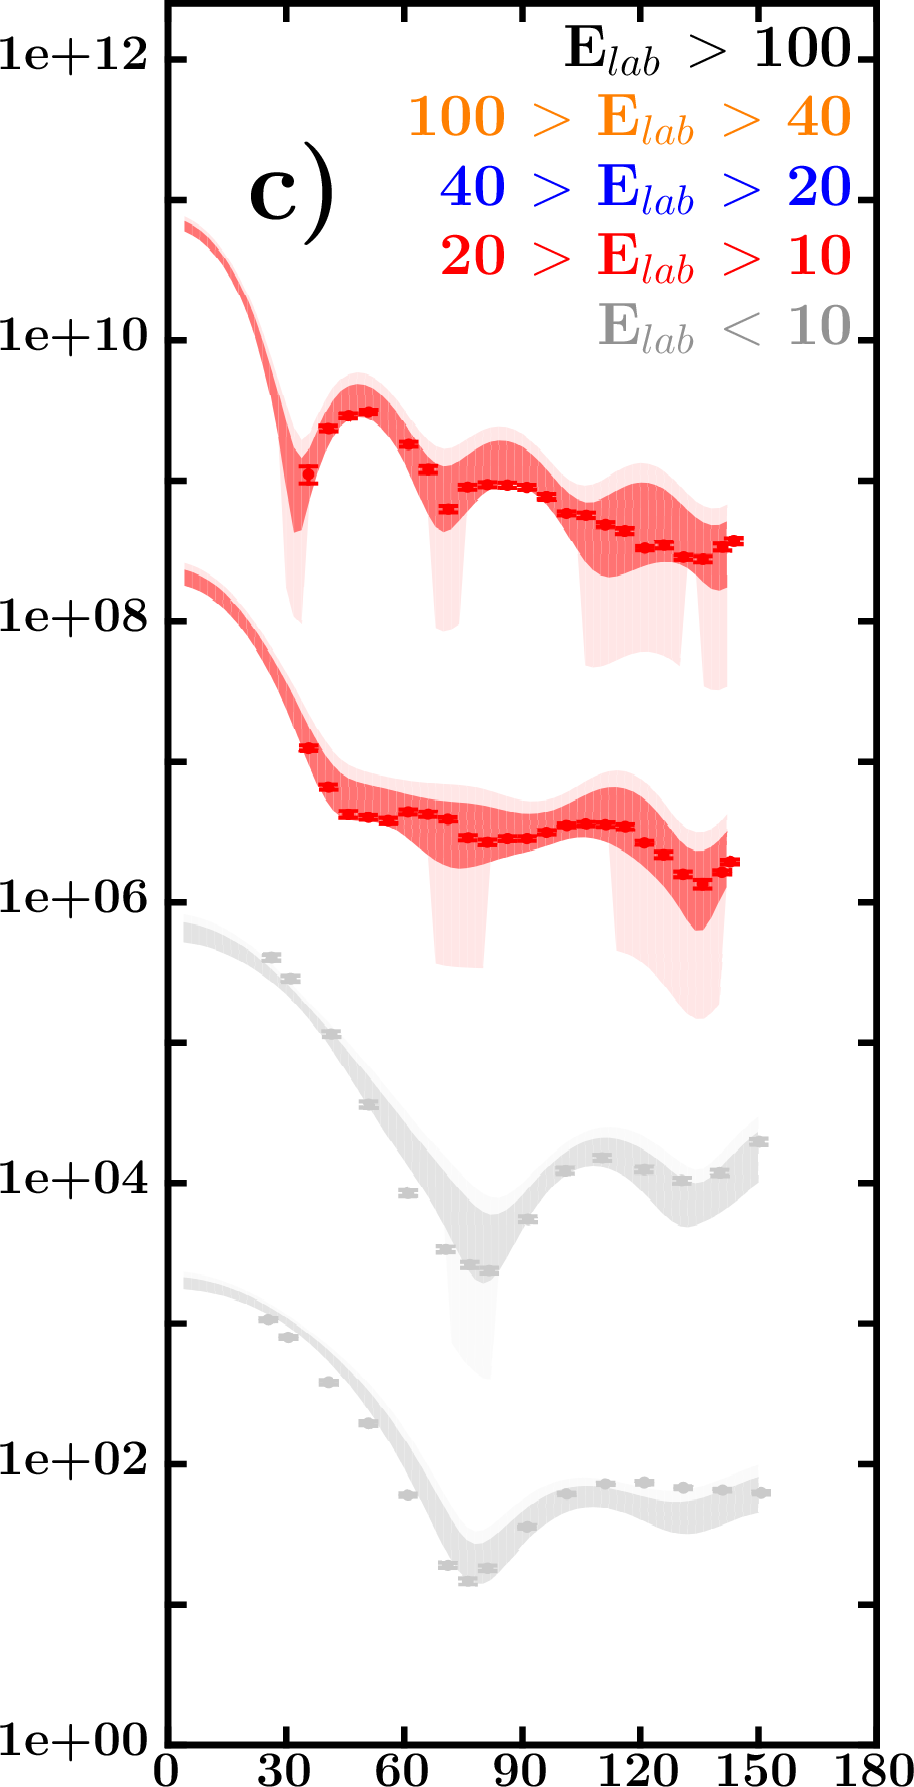
\includegraphics[width=\linewidth]{figures/ca48_neutronElastic.png}
        \label{DOM_ca48_neutron_elastic}
    \end{minipage}
    \centering
    \begin{minipage}{0.4\linewidth}
        \centering
        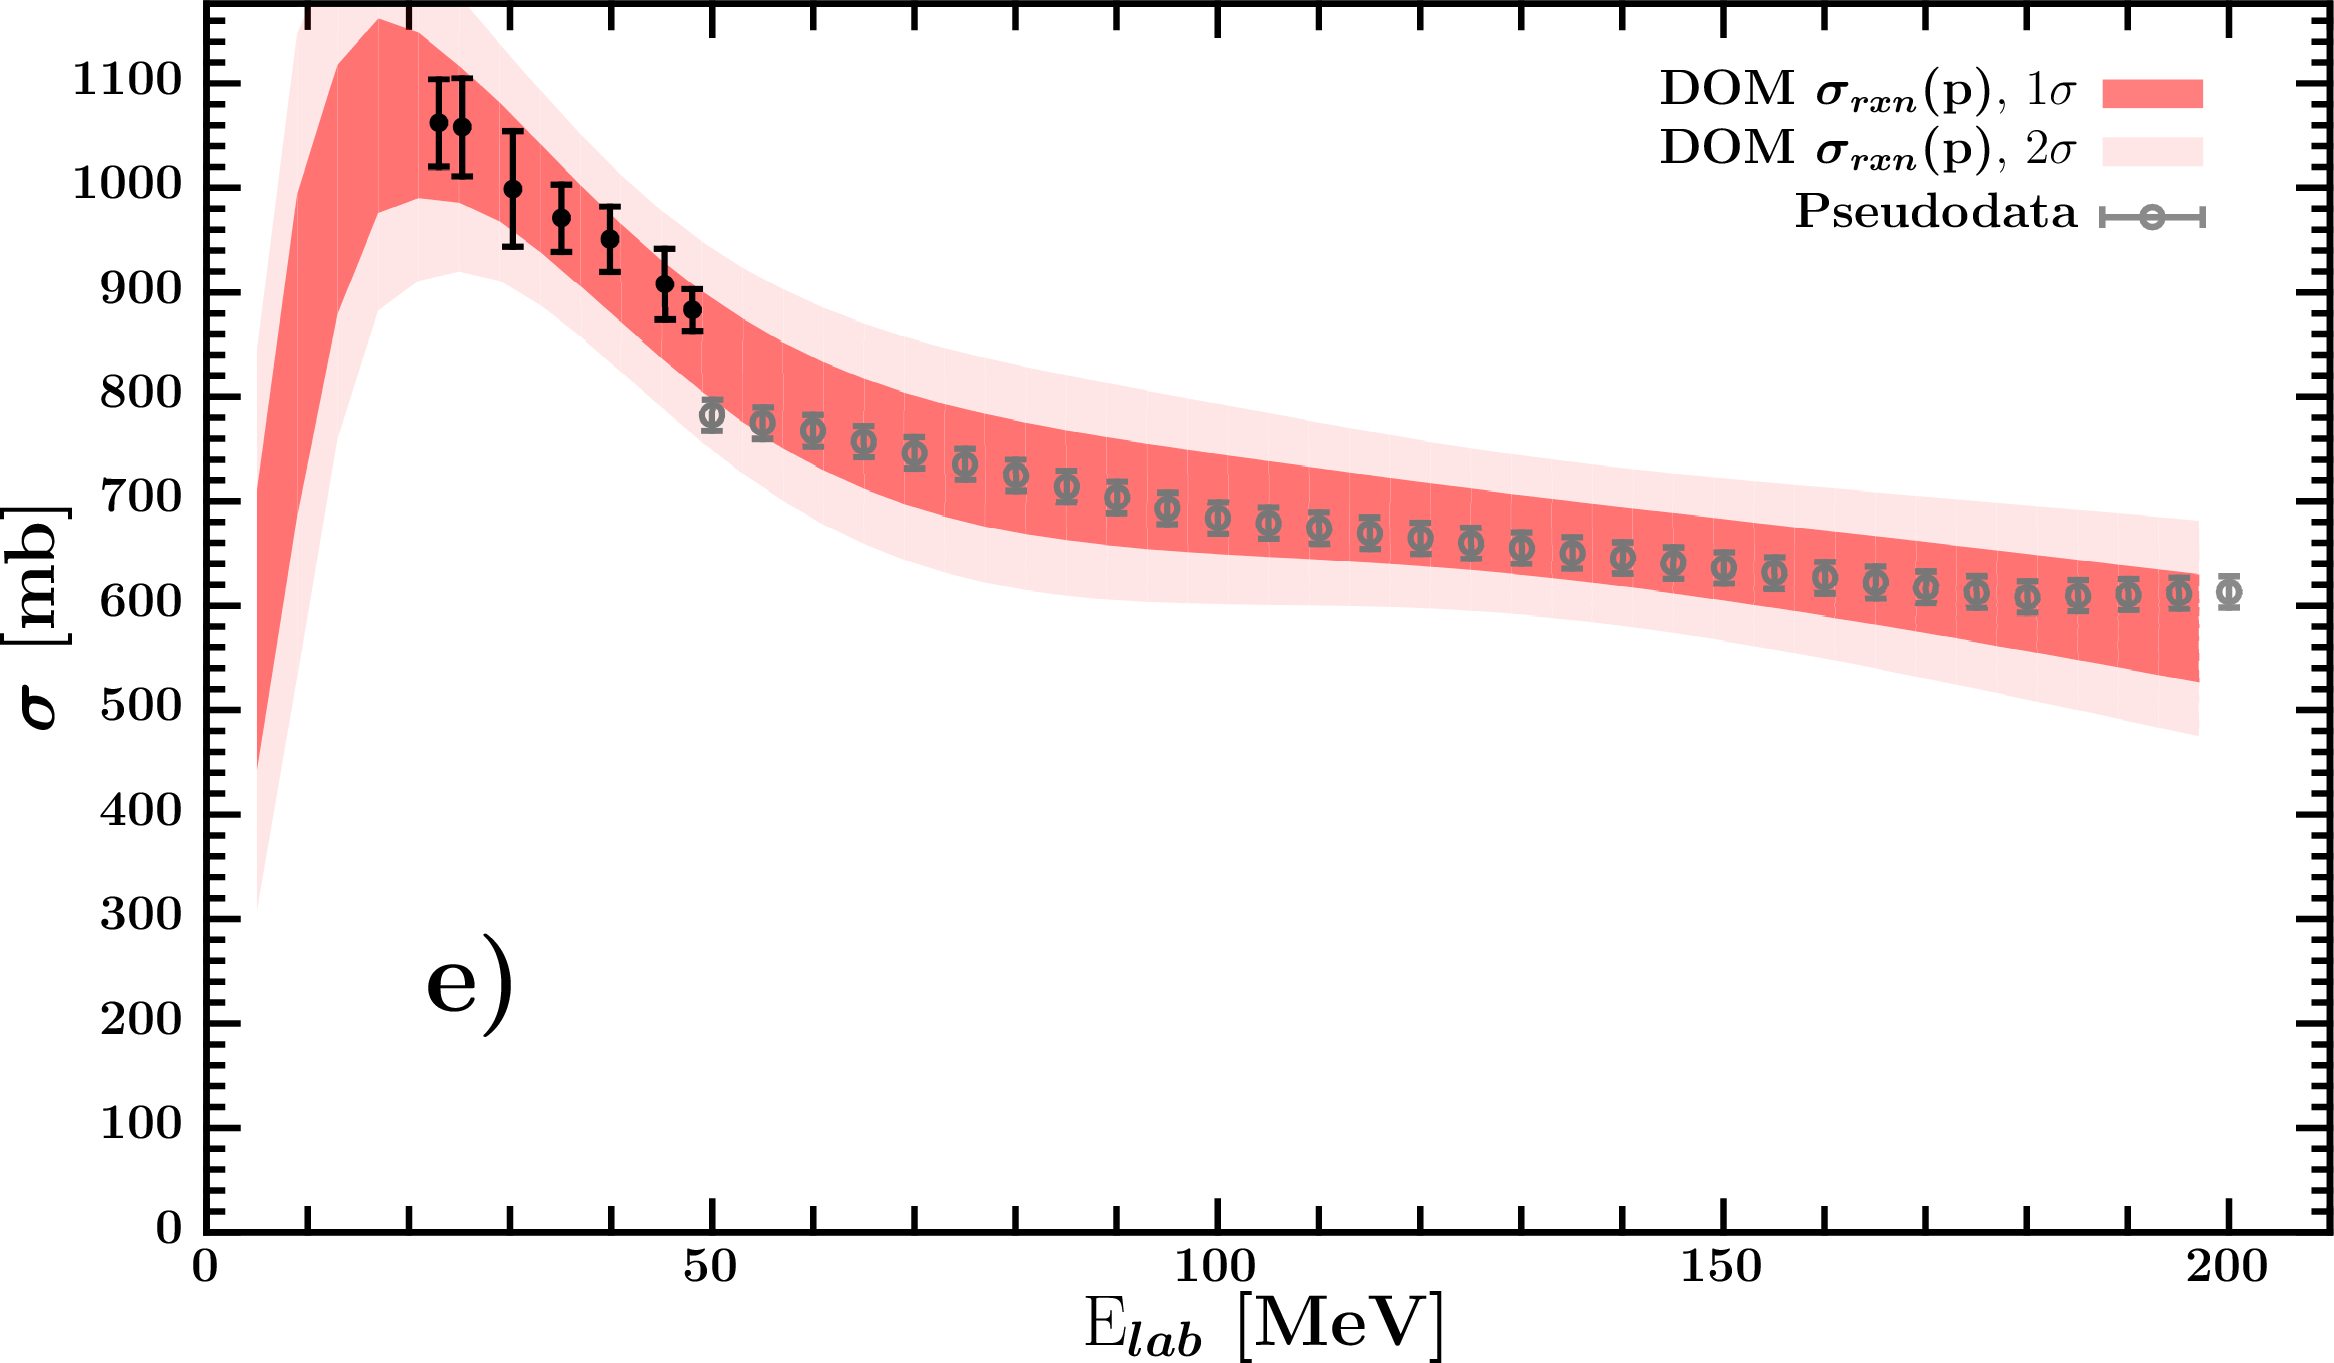
\includegraphics[width=\linewidth]{figures/ca48_protonInelastic.png}
        \label{DOM_ca48_proton_inelastic}
    \end{minipage}\hspace{6pt}
    \begin{minipage}{0.4\linewidth}
        \centering
        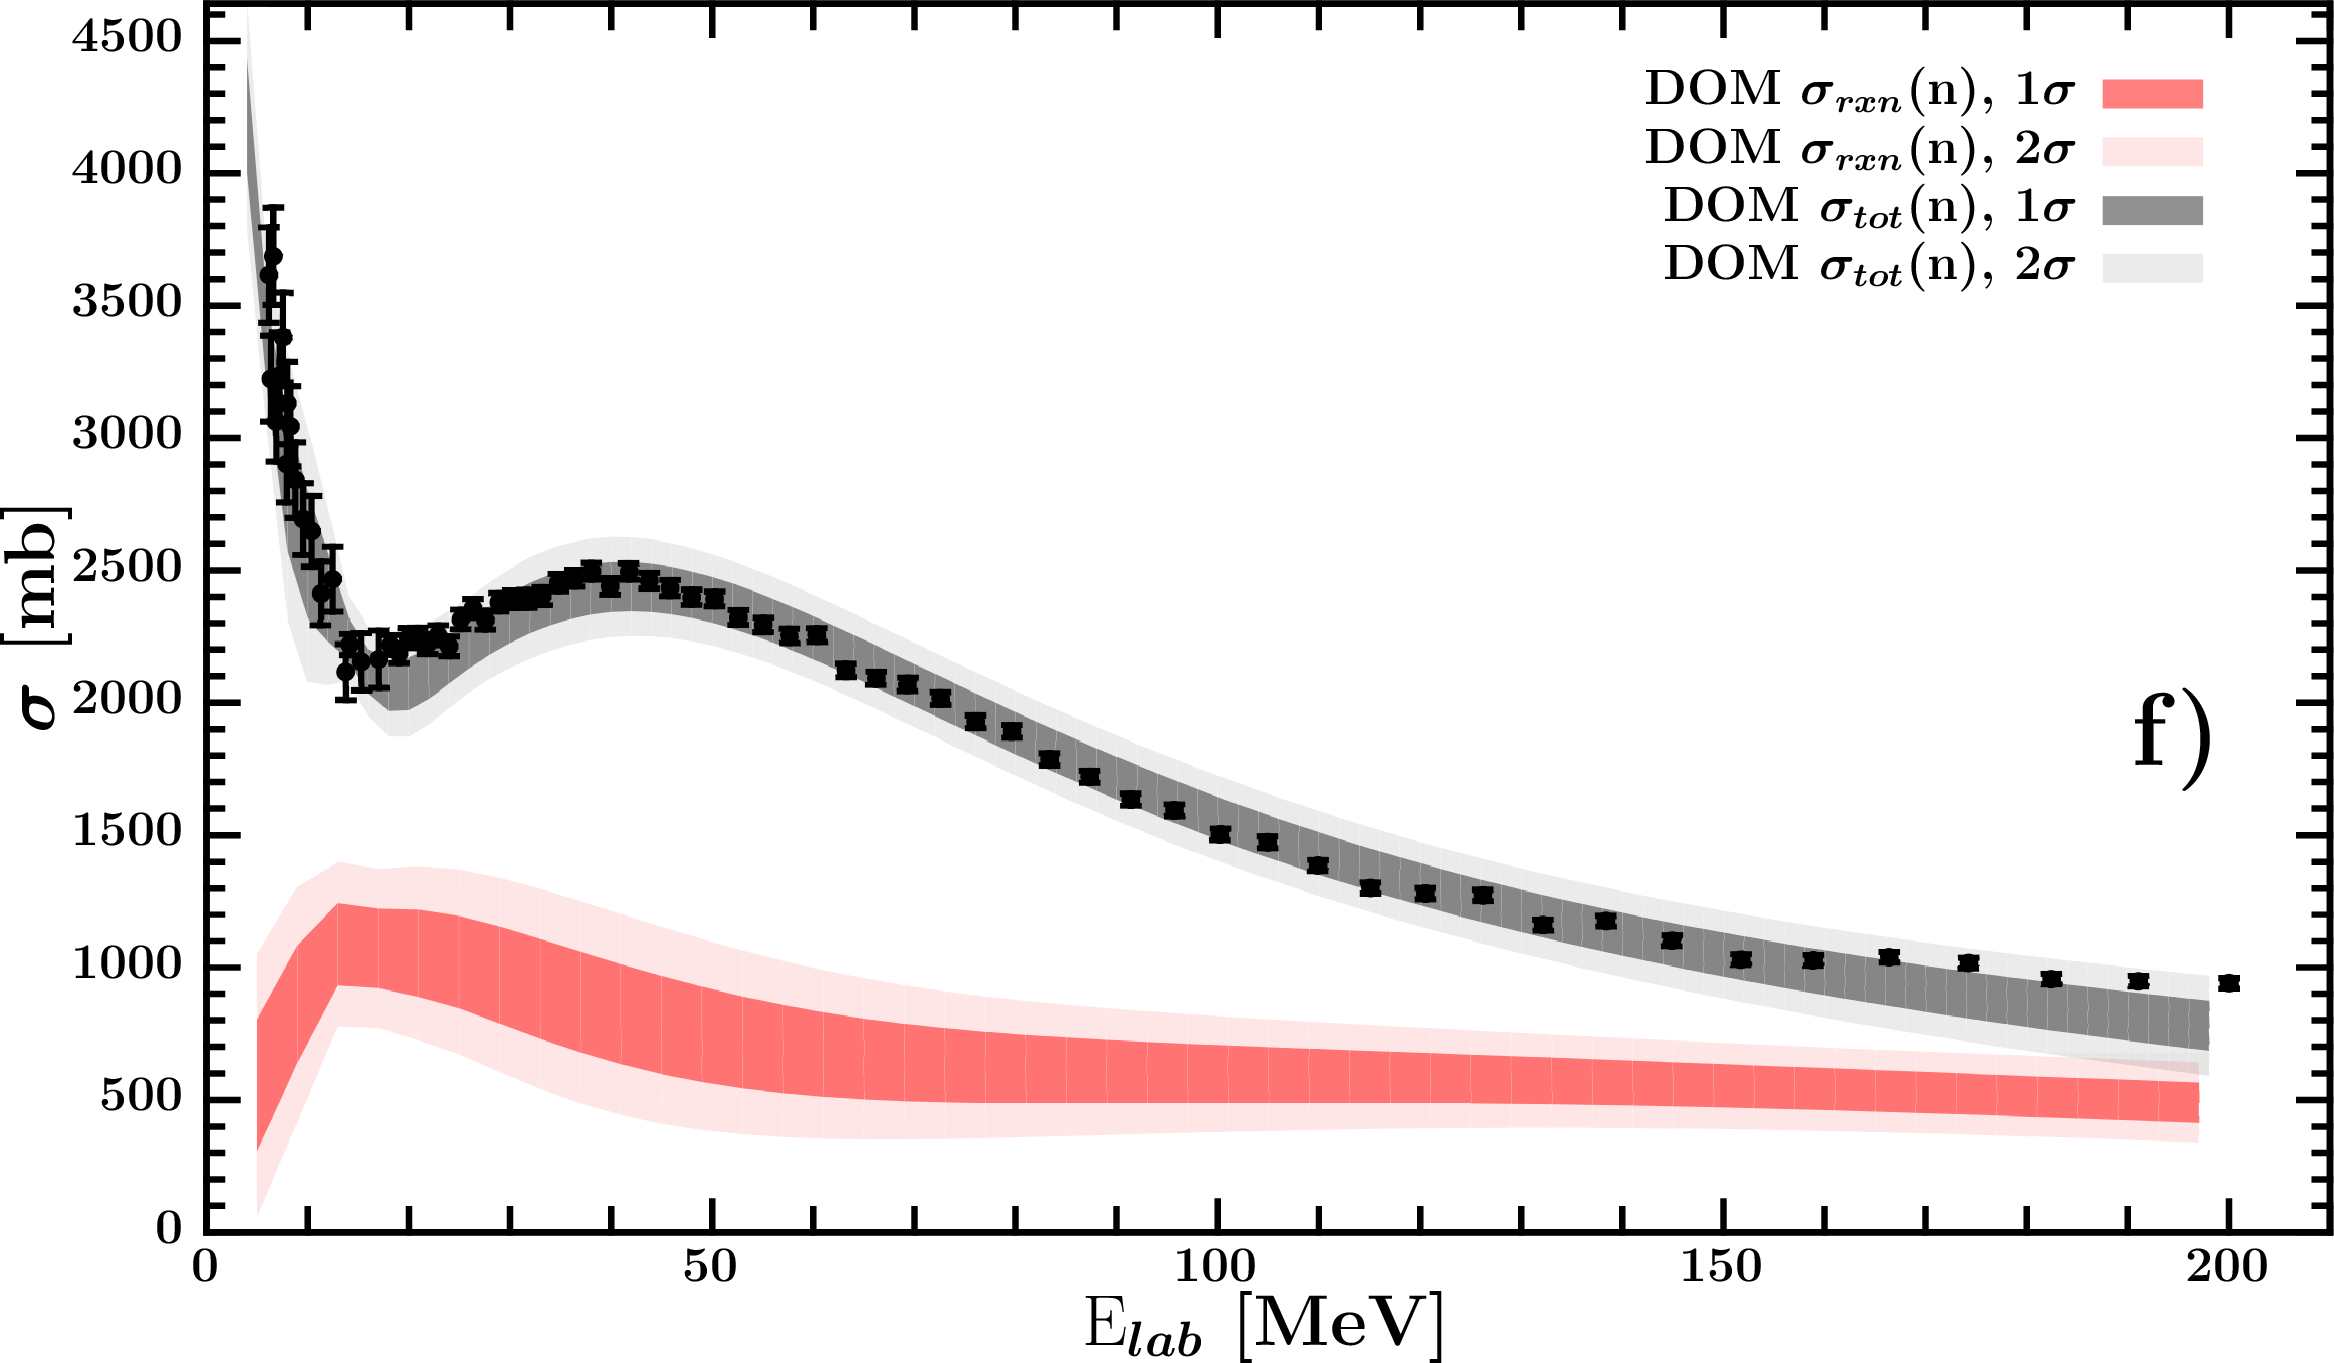
\includegraphics[width=\linewidth]{figures/ca48_neutronInelastic.png}
        \label{DOM_ca48_neutron_inelastic}
    \end{minipage}
    \caption{\caEight\ nucleon scattering data used in DOM fit}
    \label{DOM_ca48_scattering}
    \centering
    \begin{minipage}{0.4\linewidth}
        \centering
        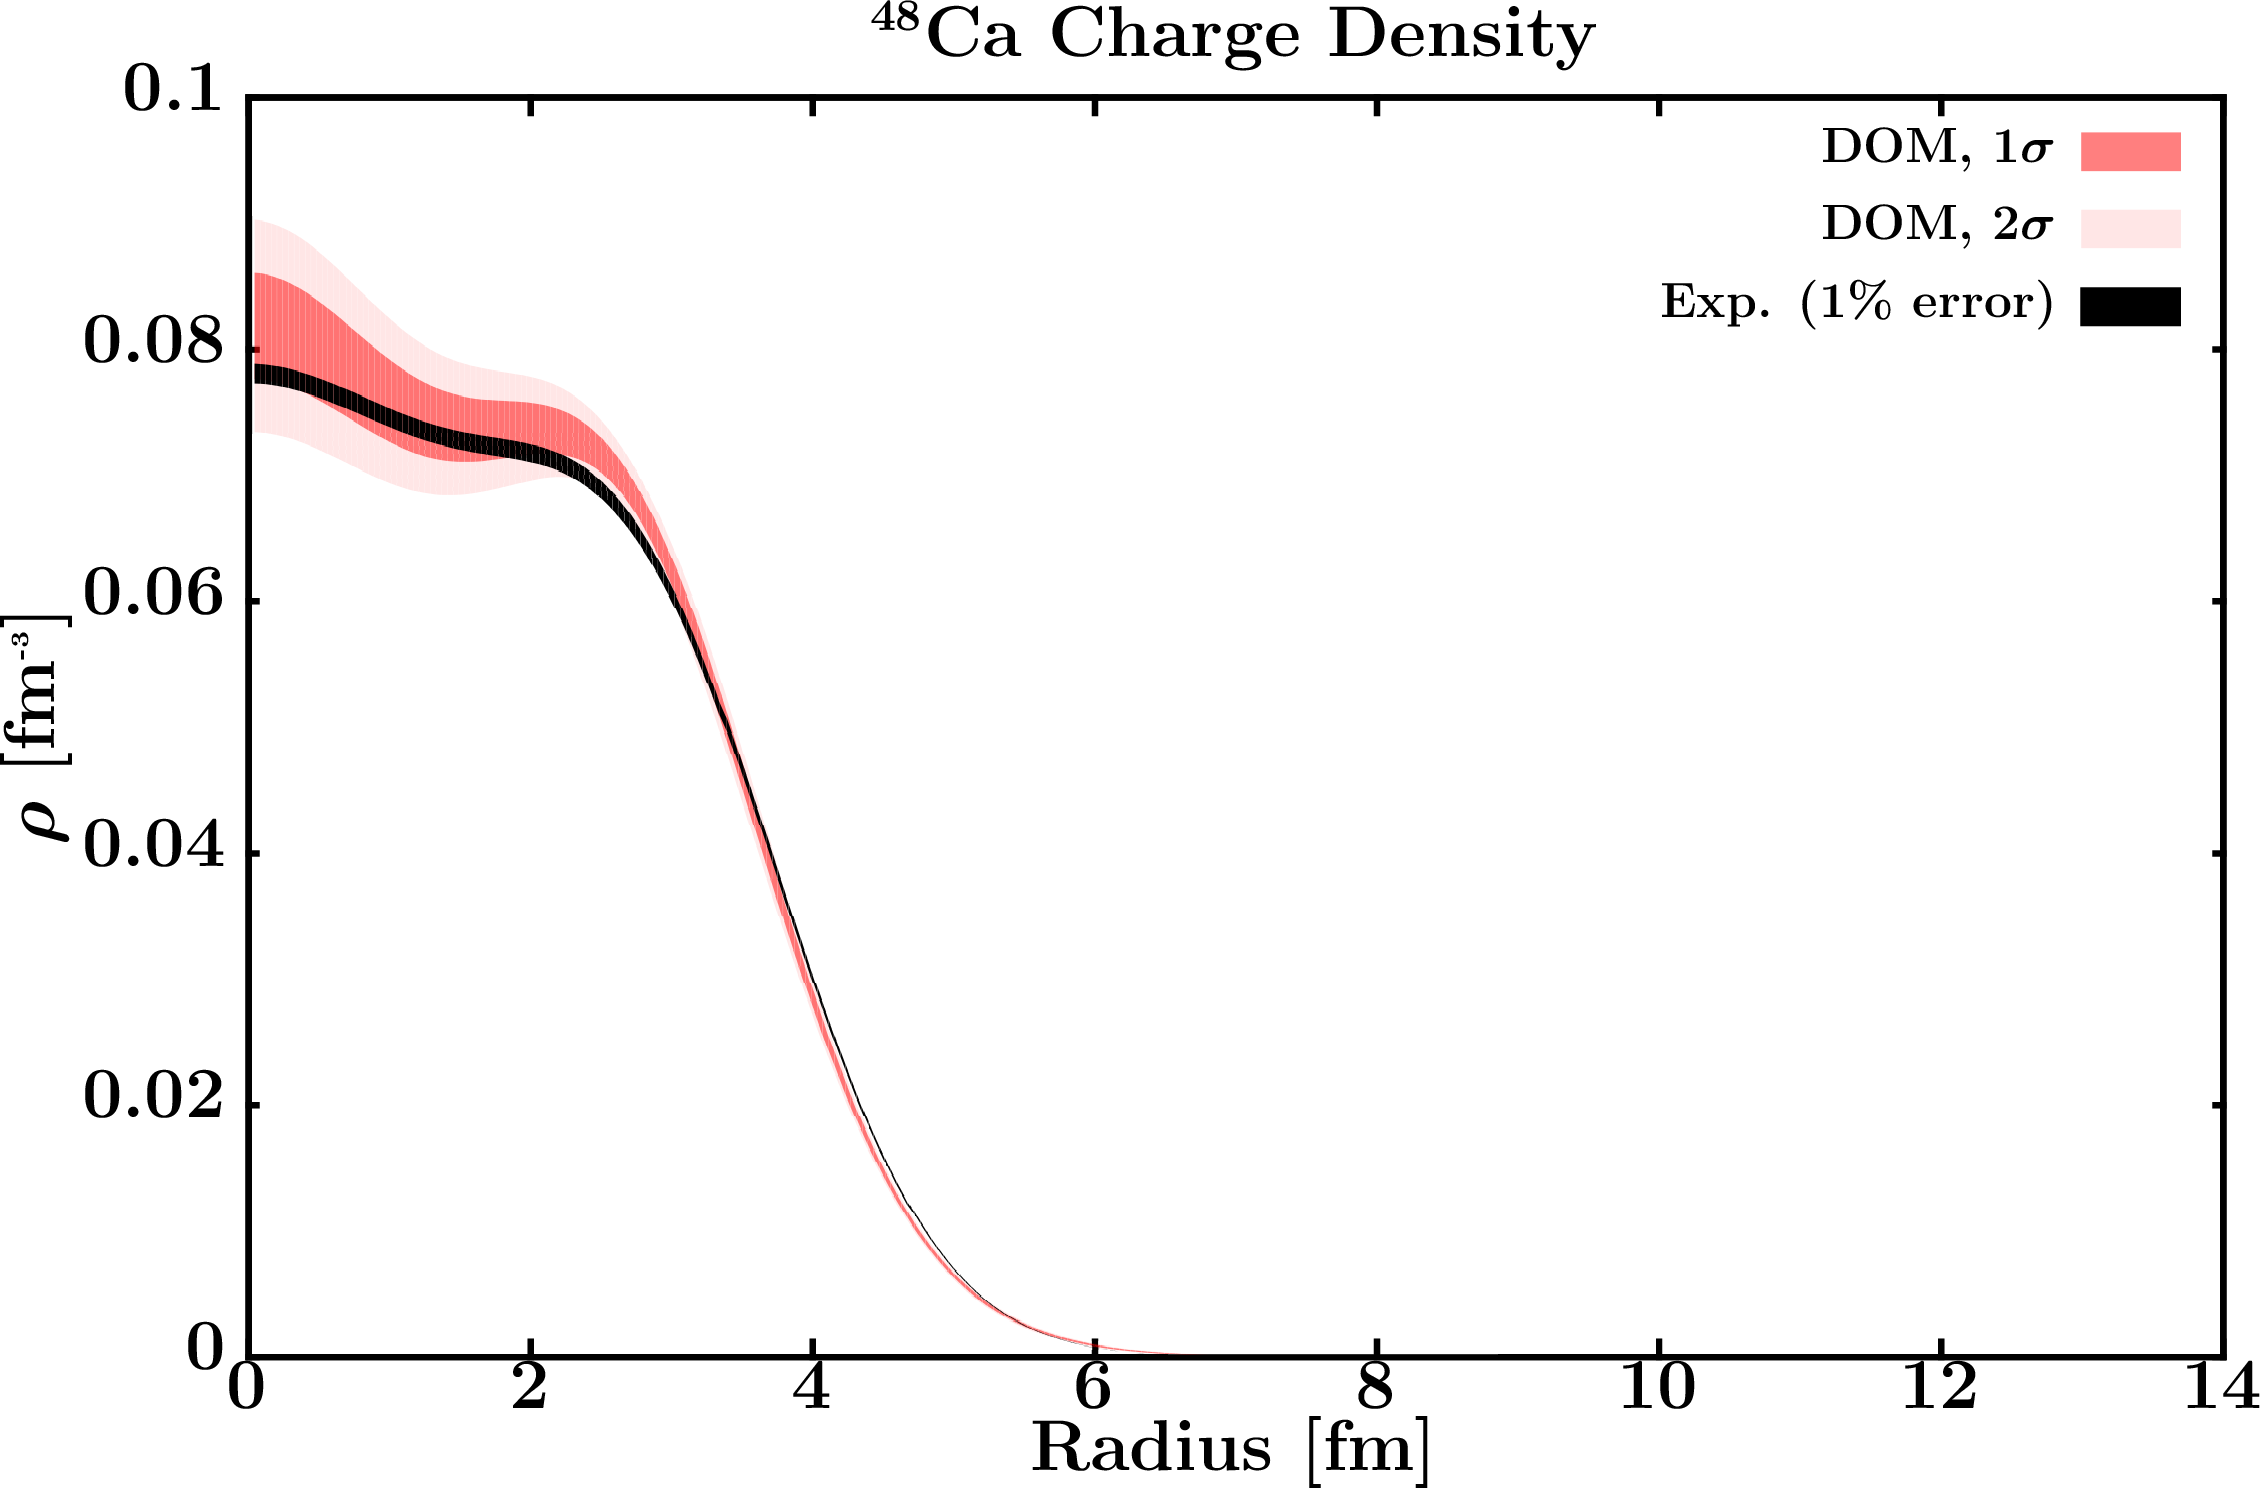
\includegraphics[width=\linewidth]{figures/ca48_chargeDensity.png}
        \label{DOM_ca48_chargeDensity}
    \end{minipage}
    \begin{minipage}{0.35\linewidth}
        \centering
        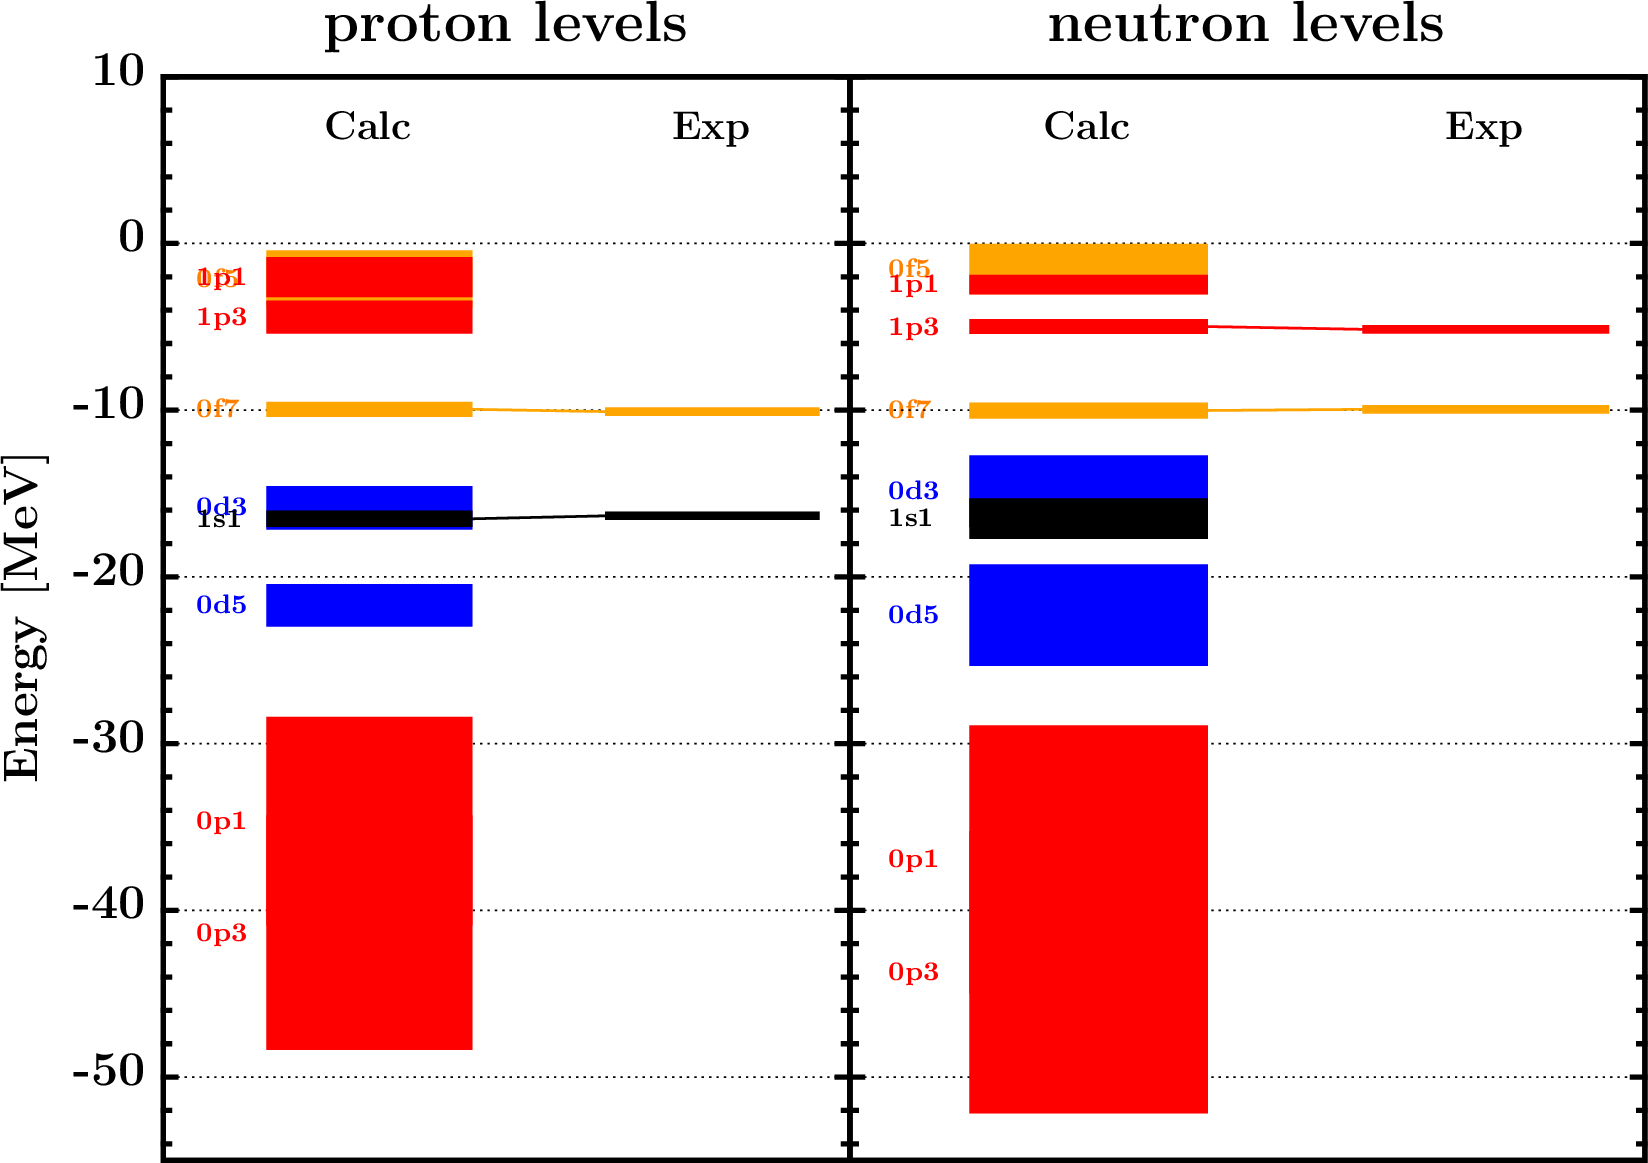
\includegraphics[width=\linewidth]{figures/ca48_SPLevels.png}
        \label{DOM_ca48_SPLevels}
    \end{minipage}
    \begin{minipage}{0.4\linewidth}
        \centering
        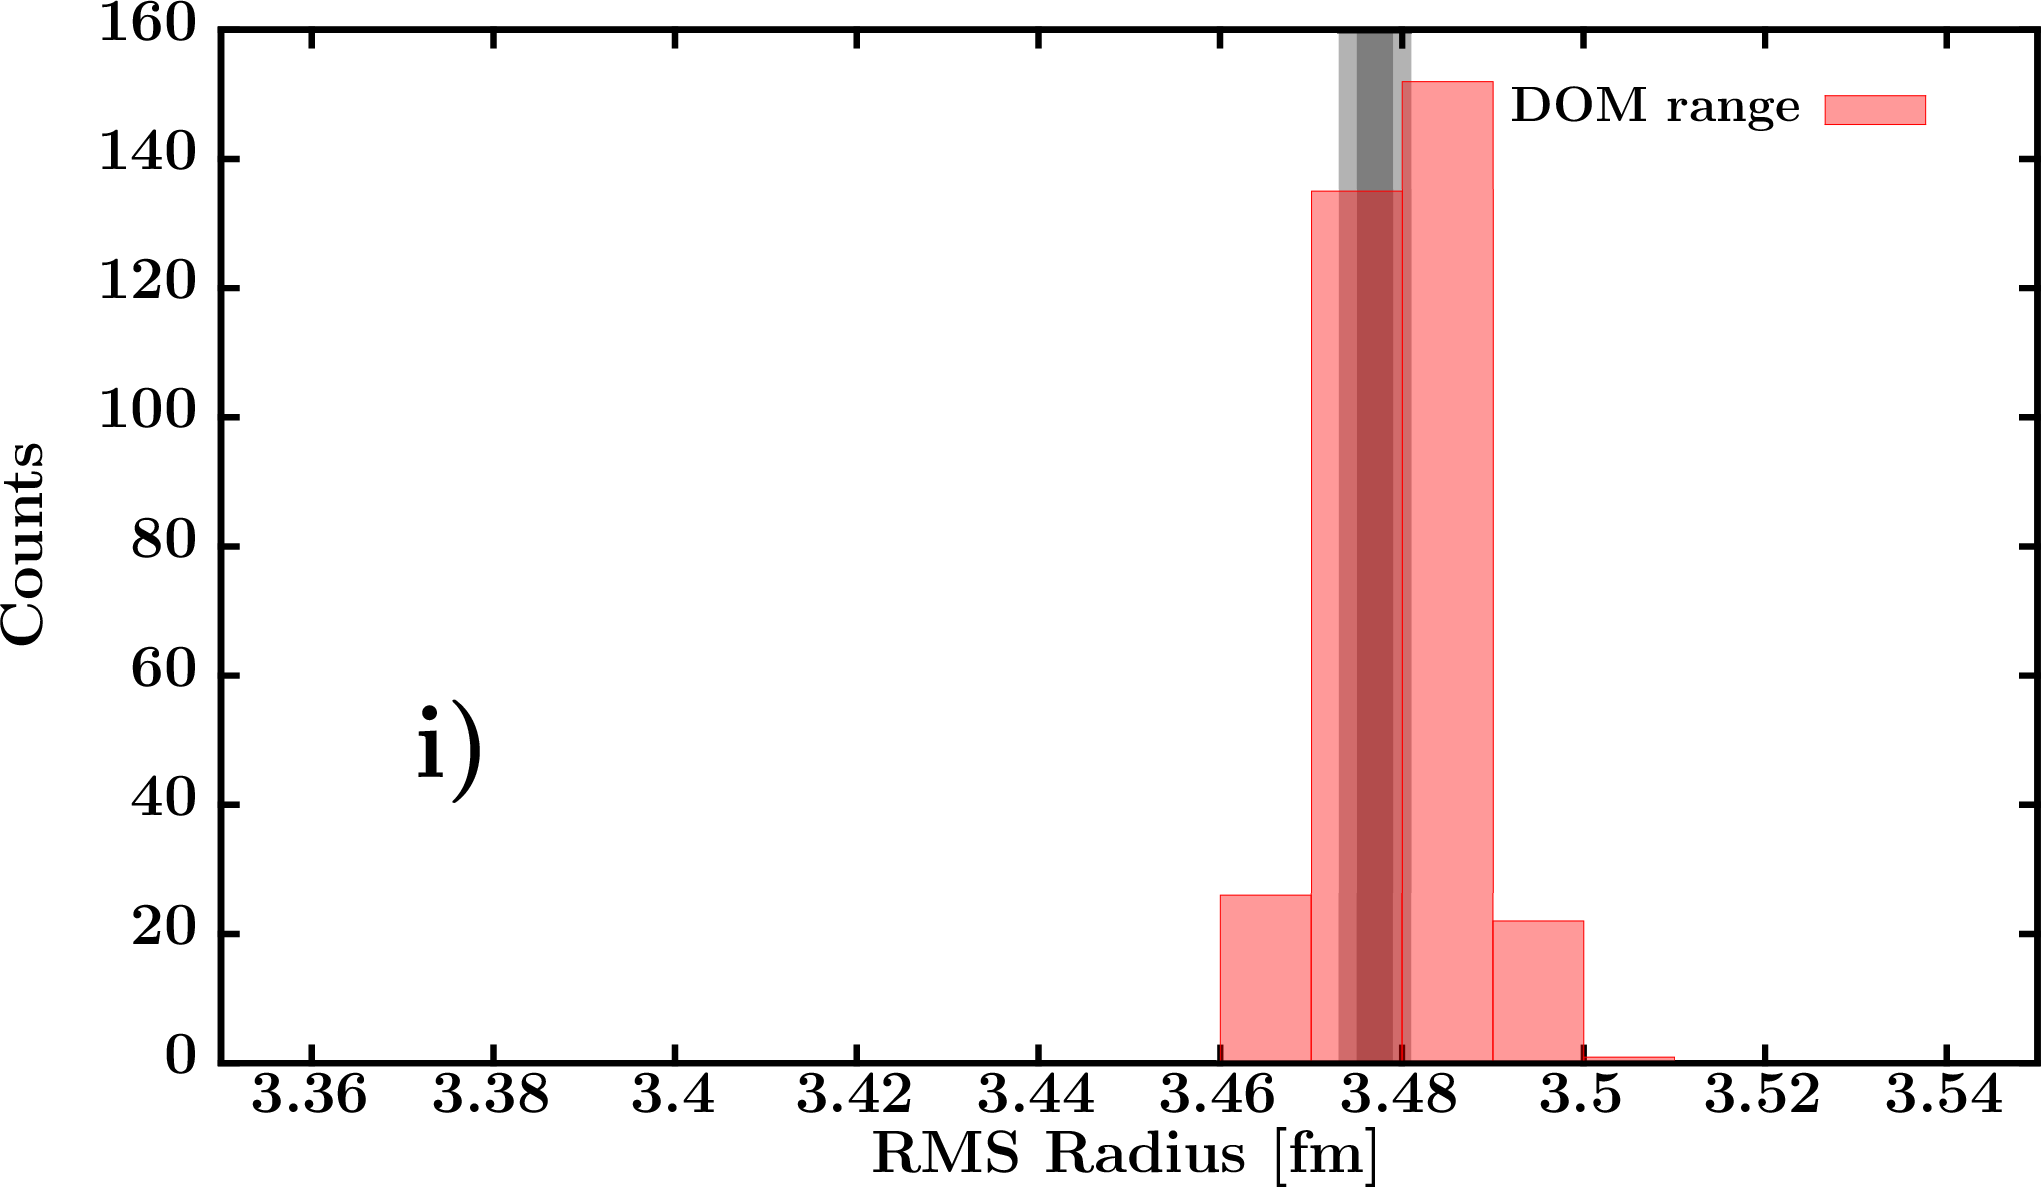
\includegraphics[width=\linewidth]{figures/ca48_RMSRadius.png}
        \label{DOM_ca48_RMSRadius}
    \end{minipage}
    \begin{minipage}{0.4\linewidth}
        \centering
        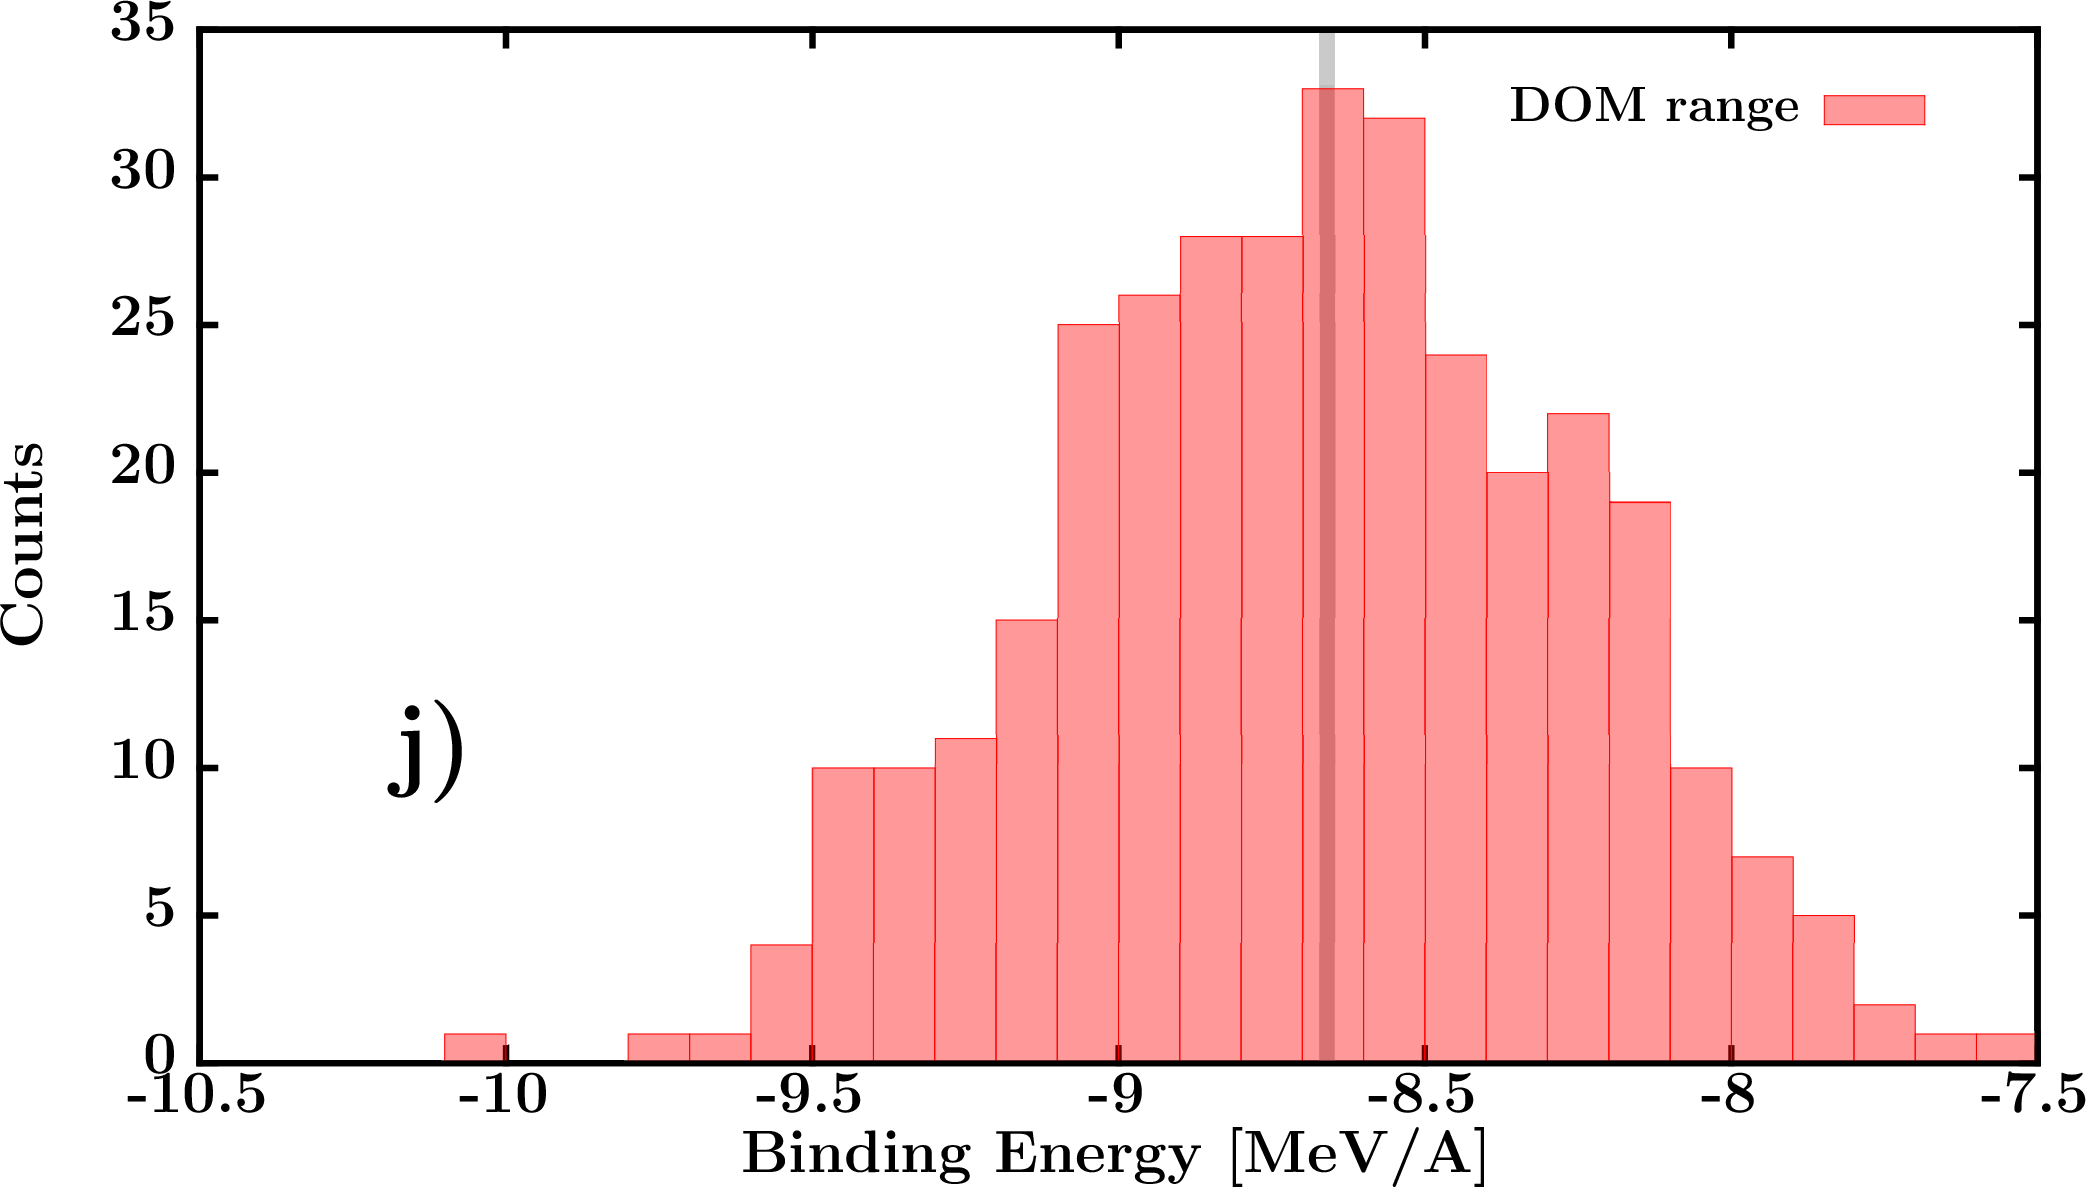
\includegraphics[width=\linewidth]{figures/ca48_BE.png}
        \label{DOM_ca48_BE}
    \end{minipage}
    \caption{\caEight\ bound-state data used in DOM fit}
    \label{DOM_ca48_structural}
\end{figure*}

\end{document}
